% **************************************************
% Document Class Definition
% **************************************************
\documentclass[%
    paper=A4,               % paper size --> A4 is default in Germany
    twoside=true,           % onesite or twoside printing
    openright,              % doublepage cleaning ends up right side
    parskip=half,           % spacing value / method for paragraphs
    chapterprefix=true,     % prefix for chapter marks
    11pt,                   % font size
    headings=normal,        % size of headings
    bibliography=totoc,     % include bib in toc
    listof=totoc,           % include listof entries in toc
    titlepage=on,           % own page for each title page
    captions=tableabove,    % display table captions above the float env
    chapterprefix=false,    % do not display a prefix for chapters
    appendixprefix=false,    % but display a prefix for appendix chapter
    draft=false,            % value for draft version
]{scrreprt}%


% **************************************************
% Setup YOUR thesis document in this file !
% **************************************************
% !TEX root = my-thesis.tex


% **************************************************
% Files' Character Encoding
% **************************************************
\PassOptionsToPackage{utf8}{inputenc}
\usepackage{inputenc}


% **************************************************
% Information and Commands for Reuse
% **************************************************
% Custom commands
\newcommand{\gaia}{\emph{Gaia}}

% Settings
\newcommand{\thesisTitle}{Detection and characterisation of open clusters in the Milky Way with \gaia}
\newcommand{\thesisName}{Emily Lauren Hunt}
\newcommand{\thesisSubject}{Observational astronomy}
\newcommand{\thesisDate}{May 2nd, 2023}
\newcommand{\thesisExamDate}{July 12th, 2023}
\newcommand{\thesisVersion}{Draft 1}

\newcommand{\thesisFirstReviewer}{PD Dr. Sabine Reffert}
\newcommand{\thesisFirstReviewerUniversity}{\protect{Ruprecht-Karls-Universität}}
\newcommand{\thesisFirstReviewerDepartment}{Zentrum für Astronomie}

\newcommand{\thesisSecondReviewer}{Prof. Dr. Hans-Walter Rix}
\newcommand{\thesisSecondReviewerUniversity}{\protect{Max-Planck-Institut für Astronomie}}
\newcommand{\thesisSecondReviewerDepartment}{Galaxies and Cosmology group}

\newcommand{\thesisFirstSupervisor}{PD Dr. Sabine Reffert}
\newcommand{\thesisSecondSupervisor}{NONE}

\newcommand{\thesisUniversity}{\protect{Ruprecht-Karls-Universität}}
\newcommand{\thesisUniversityDepartment}{Zentrum für Astronomie}
\newcommand{\thesisUniversityInstitute}{Landessternwarte Königstuhl}
\newcommand{\thesisUniversityGroup}{Extrasolar Planet Research Group}
\newcommand{\thesisUniversityCity}{Heidelberg}
\newcommand{\thesisUniversityStreetAddress}{Königstuhl 12}
\newcommand{\thesisUniversityPostalCode}{69117 Heidelberg}


% **************************************************
% Debug LaTeX Information
% **************************************************
%\listfiles


% **************************************************
% Load and Configure Packages
% **************************************************
\usepackage[english]{babel} % babel system, adjust the language of the content
\PassOptionsToPackage{% setup clean thesis style
    figuresep=colon,%
    hangfigurecaption=false,%
    hangsection=true,%
    hangsubsection=true,%
    sansserif=false,%
    configurelistings=true,%
    colorize=full,%
    colortheme=redlilac,%
    configurebiblatex=true,%
    bibsys=biber,%
    bibfile=bib-refs,%
    bibstyle=alphabetic,%
    bibsorting=nty,%
}{cleanthesis}
\usepackage{cleanthesis}

\hypersetup{% setup the hyperref-package options
    pdftitle={\thesisTitle},    %   - title (PDF meta)
    pdfsubject={\thesisSubject},%   - subject (PDF meta)
    pdfauthor={\thesisName},    %   - author (PDF meta)
    plainpages=false,           %   -
    colorlinks=false,           %   - colorize links?
    pdfborder={0 0 0},          %   -
    breaklinks=true,            %   - allow line break inside links
    bookmarksnumbered=true,     %
    bookmarksopen=true          %
}



\usepackage[]{layouts}


% **************************************************
% Document CONTENT
% **************************************************
\begin{document}

% uncomment the following command to fill up pages with
% whitespace instead of aligning the first and last lines
% of a page (see \raggedbottom vs. \flushbottom)
%\raggedbottom

% --------------------------
% rename document parts
% --------------------------
%\renewcaptionname{ngerman}{\figurename}{Abb.}
%\renewcaptionname{ngerman}{\tablename}{Tab.}
\renewcaptionname{english}{\figurename}{Fig.}
\renewcaptionname{english}{\tablename}{Tab.}

% --------------------------
% Front matter
% --------------------------
\pagenumbering{roman}			% roman page numbing (invisible for empty page style)
\pagestyle{empty}				% no header or footers
% !TEX root = ../my-thesis.tex
%
% ------------------------------------  --> book title page
% this is to be used as a cover if I ever get a nice copy of this printed.
% \begin{titlepage}
% 	\pdfbookmark[0]{Cover}{Cover}
% 	\tgherosfont
% 	\centering

% 	\vspace*{\fill}
% 	{\large \thesisUniversity} \\[5mm]
% 	{\LARGE \color{ctcolortitle}\textbf{\thesisTitle} \\[10mm]}
% 	{\Large \thesisName} \\[8cm]
% 	\vspace*{\fill}


% \end{titlepage}

% ------------------------------------  --> official HGSFP title pages
% Statement of dissertation
\begin{titlepage}
	\pdfbookmark[0]{Title Page}{Title Page}
	\centering
	\begin{large}
		Dissertation\\[5mm]
		submitted to the\\
		Combined Faculty of Mathematics, Engineering and Natural Sciences\\
		of Heidelberg University, Germany\\
		for the degree of\\[5mm]
		Doctor of Natural Sciences\\

		\hfill
		\vfill

		Put forward by\\[5mm]
		\thesisName\\
		born in: Coventry, United Kingdom\\[5mm]
		Oral examination: \thesisExamDate\\
	\end{large}
\end{titlepage}

% Title and referees
\begin{titlepage}
	\centering
	{\Large \thesisTitle}
	\hfill
	\vfill

	\begin{minipage}[t]{.3\textwidth}
		\raggedleft
		Referees:
	\end{minipage}
	\hspace*{.1\textwidth}
	\begin{minipage}[t]{.585\textwidth}
		{\thesisFirstReviewer} \\
		{\thesisSecondReviewer} \\
	\end{minipage} \\[5mm]

	\newpage
\end{titlepage}


% ------------------------------------  --> lower title back for single page layout
\hfill
\vfill
{
	\small
	\textbf{\thesisName} \\
	\textit{\thesisTitle} \\
	\thesisUniversity, \thesisDate \\
	Reviewers: \thesisFirstReviewer\ and \thesisSecondReviewer \\
	Supervisor: \thesisFirstSupervisor\\[1.5em]
	\textbf{\thesisUniversity} \\
	\textit{\thesisUniversityGroup} \\
	\thesisUniversityInstitute \\
	\thesisUniversityDepartment \\
	\thesisUniversityStreetAddress \\
	\thesisUniversityPostalCode
}
		% INCLUDE: all titlepages
\cleardoublepage

\pagestyle{plain}				% display just page numbers
% !TEX root = ../my-thesis.tex
%

\pdfbookmark[0]{Abstract}{Abstract}
\addchap*{Abstract}
\label{sec:abstract}

% --------------- ENGLISH
% 344 words

For over a century, open clusters have been a key tool for understanding stellar and galactic evolution. 
Now, thanks to groundbreaking new astrometric and photometric data from the European Space Agency's \gaia\ satellite, it is possible to study open clusters to a never before seen level of accuracy and precision. 
In this thesis, I develop and apply new methodologies to improve the census of open clusters with data from \gaia. 
I focus on using modern, efficient, and statistically rigorous techniques, aiming to maximise the reliability and usefulness of the open cluster census despite the many challenges of working with the billion-star dataset of \gaia.
Firstly, I conducted a comparative study of clustering algorithms for retrieving open clusters blindly from \gaia\ data.
I found that the previously untrialed algorithm, HDBSCAN, is the most sensitive algorithm for open cluster recovery.
Next, using this methodology, I used \gaia\ DR3 data to create the largest homogeneous catalogue of open clusters to date, recovering a total of 7167 clusters -- 2387 of which are candidate new objects. 
I developed an approximate Bayesian neural network for classifying the reliability of the colour-magnitude diagrams of the clusters in the census. 
Additionally, I used a modification of this network to infer parameters such as the age and extinction of these clusters. 
Finally, since many of the objects in my catalogue appeared more compatible with moving groups, I measured accurate masses, Jacobi radii, and velocity dispersions for these clusters, thus creating the largest catalogue of these parameters for open clusters to date. 
Using said parameters, I showed that no more than 5619 of the clusters in my catalogue are compatible with bound open clusters. 
I used my mass estimates to derive an approximate completeness estimate for the \gaia\ DR3 open cluster census, finding that the approximate 100\% completeness limit depends strongly on cluster mass. 
The results of this thesis show that it is possible to reliably create a catalogue of open clusters with a single blind search, in addition to measuring parameters for these objects. 
The methods developed in this thesis will be applicable to future data releases from \gaia\ and other sources.


% --------------- GERMAN
\newpage
%\vspace*{20mm}

{\usekomafont{chapter}Zusammenfassung}
\label{sec:abstract-diff}

Seit über hundert Jahren werden offene Sternhaufen benutzt, um stellare und galaktische Evolution zu verstehen. Dank neuer, bahnbrechender astrometrischer und photometrischer Daten des \gaia\ Satelliten der Europäischen Weltrauorganisation (ESA) ist es nun möglich offene Sternhaufen so genau wie noch nie zu untersuchen. 
In dieser Doktorarbeit entwickelte und implementierte ich neue Methodologien, um den Zensus offener Sternhaufen mit \gaia\ Daten zu verbessern. Ich konzentrierte mich auf moderne, effiziente und statistisch präzise Verfahren, mit dem Ziel, die Reliabilität und Nützlichkeit des Zensus, trotz der vielen Herausforderungen, die die Arbeit mit dem Milliarden-Sternen Datensatz von \gaia\ mit sich bringt, zu maximieren. 
Zuerst führte ich eine vergleichende Studie von Clustering- Algorithmen durch, die zur \textbf{tastende Suche} von Offenen Sternhaufen aus \gaia\ Daten genutzt werden. Anschließend, nutze ich anhand dieser Methodologie \gaia\ DR3 Daten, um den bis jetzt größten homogenen Katalog offener Sternhaufen zu erstellen. Aus den Daten gehen 7167 Sternhaufen hervor, 2387 davon (sind) \textbf{potentielle neue Objekte}. Ich entwickelte ein approximatives Bayessches Neuronennetz, um die Reliabilität \textbf{von colour magnitude diagrams} der Sternhaufen des Zensus zu klassifizieren. Außerdem benutzte ich eine Modifikation dieses Netzwerkes, um Parameter, wie das Alter und die Extinktion dieser Sternhaufen zu erschließen.
Da viele der Objekte in meine Katalog eher Sternassoziation ähneln, berechnete ich akkurate Massen, Jacobi Radii, sowie Geschiwndigkeits-Dispersion für diese Sternhaufen, und erstellte somit den größten Katalog der oben genannten Parameter für offene Sternhaufen bisher. 
Anhand der Parameter zeigte ich, dass lediglich 5619 der Sternhaufen in meinem Katalog gebundenen offenen Sternhaufen entsprechen. 
Ich benutzte meine Masse-Schätzungen, um eine approximative Gesamtheitsestimat für den \gaia\ DR3 Zensus offener Sternhaufen abzuleiten und fand heraus, dass das approximative 100\% Gesamtheitslimit stark von der Masse der Sternhaufen abhängt. 
Die Ergebnisse dieser Arbeit zeigen, dass es möglich ist, verlässlich einen Katalog offener Sternhaufen mit einem einzelnen tastenden Suchlauf zu erstellen und außerdem die Parameter der Objekte zu messen. 
Die in dieser Arbeit entwickeltem Methoden werden auf zukünftige Datensätze von \gaia\ sowie anderen Quellen anwendbar sein. 
		% INCLUDE: the abstracts (english and german)
\cleardoublepage
%
% !TEX root = ../my-thesis.tex
%
\pdfbookmark[0]{Acknowledgement}{Acknowledgement}
\addchap*{Acknowledgement}
\label{sec:acknowledgement}

\Blindtext[2][2]
 % INCLUDE: acknowledgement
\cleardoublepage
%
\currentpdfbookmark{\contentsname}{toc}
\setcounter{tocdepth}{2}		% define depth of toc
\tableofcontents				% display table of contents
\cleardoublepage

% --------------------------
% Body matter
% --------------------------
\pagenumbering{arabic}			% arabic page numbering
\setcounter{page}{1}			% set page counter
\pagestyle{scrheadings}			% header and footer style

%% Uncomment the following lines using the \part command
%% to add part sections
%\part{Example Part}
% !TEX root = ../my-thesis.tex
%
\chapter{Introduction}
\label{sec:intro}

\cleanchapterquote{
	\textgreek{Δέδυκε μὲν ἀ σελάννα}\\
	\textsuperscript{The moon and the Pleiades}\\
	\textgreek{καὶ Πληΐαδες, μέσαι δέ}\\
	\textsuperscript{have set, it is}\\
	\textgreek{νύκτες, πάρα δ' ἔρχετ' ὤρα,}\\
	\textsuperscript{midnight, time is passing,}\\
	\textgreek{ἔγω δὲ μόνα κατεύδω.}\\
	\textsuperscript{but I sleep alone.}\\
}{Sappho, `The Midnight Poem'}{(c. 600 BC)}

% ---------------------------------------
\section{From seven sisters to a powerhouse of astronomy}
\label{sec:intro:intro}

In all of astronomy, few objects have retained relevance throughout the centuries as much as open clusters (OCs). Easily visible to the naked eye, the Pleiades has been observed since at least the dawn of civilisation CITEME, along with a handful of other OCs visible without a telescope. In the present day, the now thousands of known OCs are a key tool in modern astronomy for understanding stellar and galactic evolution.

Star clusters are formed when clouds of cold molecular gas collapse due to gravity, forming stars. Sometimes, when star formation occurs densely enough, these stars fall further into gravitationally bound clusters that can survive in the galactic disk for as long as $\sim 10^9$~years \citep{lada_embedded_2003,portegies_zwart_young_2010}. It is this property of the formation of OCs that makes them so useful: all stars in an OC will have the same age and initial composition, allowing parameters of the overall group of stars to be measured significantly more precisely than when studying stars in isolation. 

For instance, when a parameter such as the distance of member stars can simply be averaged over all member stars, then the precision of the mean distance of an OC (and hence the distance to all of its member stars) will be a factor $\sqrt{n}$ more precise than the distance to any individual star. Alternatively, when a property such as chemical composition is highly time consuming to derive, it can be derived for a fraction of stars in an OC and be applied to all stars in a cluster.

The ease of studying stellar astrophysics with OCs results in OCs having an extremely wide range of scientific use cases. For instance, OCs are used as testing grounds for stellar evolution models CITEME, as tracers of galactic structure \citep{cantat-gaudin_painting_2020,castro-ginard_milky_2021}, or even as calibrators of Cepheid variable stars \citep{medina_revisited_2021}, which are an essential first rung on the cosmic distance ladder and are vital in the derivation of the cosmological parameters of the universe. It is somewhat of a cliché to describe OCs as `the laboratories of stellar evolution', but it really is true: OCs are a fantastic way to observe stars of a given age and composition across a broad range of masses, and to do so with orders of magnitude more precision than when studying isolated field stars.

The best part of the modern story of the OC's contribution to astrophysics comes with the \gaia\ satellite, however. In just five years since its first full data release \citep{brown_gaia_2018}, \gaia\ has revolutionised the study of our galaxy, including the study of OCs; with dozens of papers reporting thousands of new objects \citep[e.g.][]{liu_catalog_2019,castro-ginard_hunting_2019,castro-ginard_hunting_2020,castro-ginard_hunting_2022}, and a number of works deriving dramatically improved parameters and members for OCs in the Milky Way \citep[e.g.][]{cantat-gaudin_gaia_2018,tarricq_3d_2020}. Arguably, there has never been a better time to do science with OCs, owing to the incredible quantity and quality of data that \gaia\ has provided.

There is, however, a catch. Even though the Milky Way is estimated to contain as many as $10^5$ OCs \citep{dias_new_2002}, there are still only a few thousand currently known in the literature -- representing a small fraction of the total number of OCs in our galaxy. It has been shown that the census of OCs is incomplete within even 1~kpc from the Sun \citep[e.g.][]{castro-ginard_new_2018}, and the extent of the remaining incompleteness is unknown. Worse still, it has been shown that many of the OCs catalogued previously in the literature may not exist \citep{cantat-gaudin_clusters_2020,piatti_catching_2023}, with it being largely unknown which OCs are or are not real. The many fantastic uses of OCs in other areas of astronomy are contingent on a reliable, accurate, and complete census of OCs; and the many current caveats with the census of OCs limit the science potential of these fantastic objects in a time when we have more available data with which to study them than ever before.

% TODO: this paragraph is too weak
In this thesis, I will present solutions to a number of the current issues with the OC census in the era of \gaia, using a range of data analysis and parameter inference techniques. I will then use these techniques to create the largest census of OCs to date and derive a range of parameters for these OCs. With this thesis, I also hope to present methods that could continue to be used to maximise the quality of the OC census for the coming decade of \gaia\ data releases -- as well as for whatever instruments supercede \gaia\ in the future.

Before launching into the chapters detailing my work over the past three and a half years, it is worth first conducting an overview of the science behind OCs in the introduction to this thesis. In Sect.~\ref{sec:intro:pre-gaia}, I will discuss the history of OC observations up to before the release of \gaia\ DR2 in 2018, as well as briefly discussing the techniques and results from pre-\gaia\ observations. Section~\ref{sec:intro:gaia} will then discuss the stunning data of \gaia\ and how it has already thoroughly revolutionised our understanding of OCs in just a handful of years. Finally, Sect.~\ref{sec:intro:theory} will briefly discuss some key pieces of theory surrounding the structure, dynamics, and lifetime of OCs, providing a good background on our theoretical knowledge of OCs that will assist with the reading of this thesis.

The nomenclature and definition of star clusters varies throughout the literature. Hence, in the next section, I will quickly discuss a definition of OCs that I will adopt throughout the rest of this work.


% ---------------------------------------
\section{The definition of an open cluster}
\label{sec:intro:definition}

\begin{figure}[tb]
	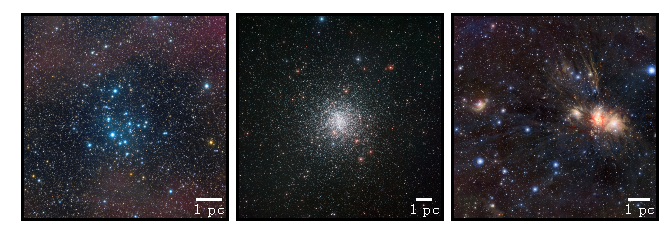
\includegraphics[width=\textwidth]{fig/c1/oc_gc_mg_comparison.pdf}
	\caption[A visual comparison between the three main types of star cluster found in the Milky Way]{A visual comparison between the three main types of star cluster found in the Milky Way. \emph{Left:} the open cluster NGC~2547. \emph{Middle:} the globular cluster M~4. \emph{Right:} the moving group/OB association Monoceros~R2. All images contain a scale in the bottom right showing a length of 1~pc at the distance of each cluster. \emph{Credit, left to right:} ESO / J. Pérez; ESO; ESO / J. Emerson / VISTA. }
	\label{fig:intro:definition:comparison}
\end{figure}

There are many different types of star cluster in the universe. Avoiding confusion when talking about star clusters is important, particularly since observers and theorists often use very different nomenclature. Definitions of star clusters can differ significantly even in observational communities when comparing between galactic and extra-galactic astronomy. Hence, before going any further, it is important to define exactly what I will be discussing in this thesis; I will use the following definitions consistently throughout this thesis for clarity.

This thesis will almost exclusively discuss clusters observed in the Milky Way, which are traditionally divided into three broad categories. I will primarily discuss open clusters, although I will also touch on globular clusters and moving groups. I differentiate between these three types of cluster approximately as follows, matching the observational definitions in \cite{portegies_zwart_young_2010}.

\textbf{Open clusters} (OCs) are gravitationally bound clusters with a typical age of around 100~Myr, although some are older than 1~Gyr and some are as young as 0.1~Myr. OCs have masses of typically no greater than $10^4$~\MSun and may be made up of a few dozen to a few thousand stars, with a typical minimum being ten stars. OCs are remants of recent star formation and are hence predominantly located in the galactic disk where the star formation rate is highest. Most OCs have a size of around 3 to 10~pc. Other than some exceptions, OCs contain a single population of stars. 

\textbf{Globular clusters} (GCs) are much older and more massive gravitationally bound clusters, with ages typically greater than 10~Gyr and masses typically greater than $10^5$~\MSun. The largest GCs can contain a million stars or more. GCs have a typical size around 10 to 20~pc. GCs tend to reside in the galactic bulge or in the galactic halo. Many GCs contain multiple populations of stars. Almost all OCs have masses significantly lower than the typical present day mass of GCs, although observations of a handful of young massive clusters in the Milky Way such as Westerlund~1 (sometimes also referred to as `super star clusters') as well as observations of galaxies with more active star formation suggest that the highest mass star clusters will be long-lived and will evolve into GCs. However, this is not the case for almost all OCs that I will study in this thesis, as the only young massive clusters in the Milky Way are generally distant, heavily reddened, and outside of the reach of the visual-band observations of the \gaia\ telescope.

\textbf{Moving groups} (MGs) are of a similar mass and number count to OCs, except they are not gravitationally bound. Due to this, they disperse much more quickly, and hence often have much younger ages. MGs have the widest definition, and encompass any group of stars that are comoving and coeval, but are specifically \emph{not} gravitationally bound. Some MGs are also referred to as `OB associations' in the literature, due to them often containing a number of young, high mass O and B stars. 

\begin{table}[tb]
	\begin{tabularx}{\textwidth}{l | X | X | X | X}
		\hline\hline
		Type & Bound? & Age & Mass & Location \\
		\hline
		Open cluster (OC)   & Weakly & $\lesssim 1$ Gyr & $\lesssim 10^4$ \MSun & Disk \\
		Globular cluster (GC)   & Strongly & $\gtrsim 10$ Gyr & $\gtrsim 10^5$ \MSun & Halo/Bulge \\
		Moving group (MG)   & No & $\lesssim 50$ Myr & $\lesssim 10^3$ \MSun & Disk\\
		\hline
	\end{tabularx}
	\caption{Approximate definitions for the three types of star cluster that will be discussed in this thesis.\label{tab:intro:definition:definition}}
\end{table}

These definitions are summarised in Table~\ref{tab:intro:definition:definition} and compared visually in Fig.~\ref{fig:intro:definition:comparison}. The figure shows three clusters; NGC~2547, M~4, and Monoceros~R2. NGC~2547 is a sparser OC that has a clear core of young blue stars at its center, about $\sim 1$~pc across. On the other hand, despite being only slightly larger, the GC M~4 clearly contains significantly more stars. The stars in M~4 are older, with the cluster having a whiter, redder appearance. Finally, the MG Monoceros~R2 is simply a group of young blue stars, with no discernible core. 





% ---------------------------------------
\section{The pre-\gaia\ history of open cluster observations}
\label{sec:intro:pre-gaia}

% Plot of the pleiades
\begin{figure}[tb]
	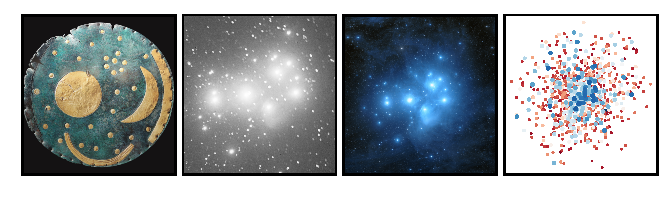
\includegraphics[width=\textwidth]{fig/c1/pleiades.pdf}
	\caption[The Pleiades as depicted throughout history]{The Pleiades, as depicted throughout history and showing the clear improvements in astronomical data gathering over time. \emph{Left:} the Nebra Sky Disc, depicting the Pleiades with its seven naked-eye visible stars in the upper center. The disc was discovered in 1999 in northern Germany and is dated to between 1800-1600 BC. \emph{Middle left:} the Pleiades, as imaged in 1909 with Wolf's Doppelastrograph at the Landessternwarte Heidelberg-Königstuhl. \emph{Middle right:} the Pleiades, as imaged by Hubble. \emph{Right:} the $\sim$1000 member stars for the Pleiades extracted from \gaia\ DR2 data and isolated from field stars by \cite{cantat-gaudin_characterising_2018}. Each star is represented by a point scaled by its magnitude and coloured according to its $BP-RP$ colour. \emph{Credits:} Frank Vincentz; Heidelberg Digitized Astronomical Plates; Davide De Martin \& NASA/ESA Hubble.}
	\label{fig:intro:history:pleiades}
\end{figure}

While the results of this thesis are entirely derived using data from \gaia\ , to truly understand just how groundbreaking the current data of the \gaia\ satellite is, it is worth first briefly reviewing the history of OC observations.


\subsection{Open clusters up to the 20th century}

Our ability to observe OCs has progressed incredibly far throughout the history of astronomy (Fig.~\ref{fig:intro:history:pleiades}). The invention of the refracting telescope allowed for early astronomers such as Galileo to observe that OCs and GCs are in fact clusters of many stars, as opposed to being dispered single sources as previously believed from unaided observations. It was, however, the invention and widespread adoptation of the reflecting telescope in the 17\textsuperscript{th} and 18\textsuperscript{th} centuries that led to catalogues of clusters like we use today.

% Plot of catalogues of OCs
\begin{figure}[tb]
	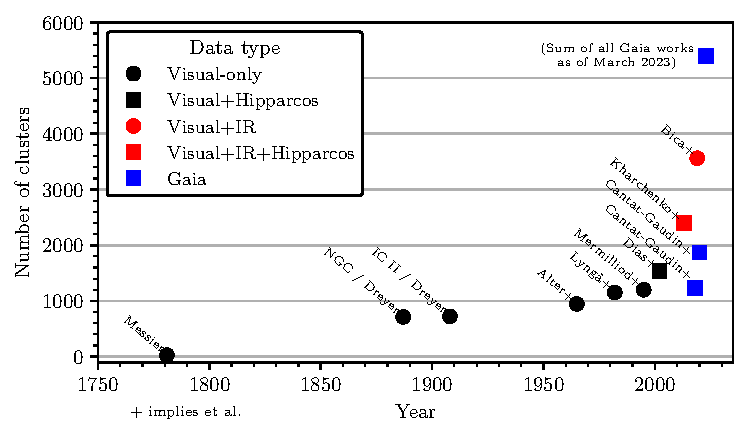
\includegraphics[width=\textwidth]{fig/c1/catalogues.pdf}
	\caption[The size of OC catalogues over time]{The size of OC catalogues over time. After the initial rise in the size of catalogues due to the advent of reflecting telescopes in the 18\third\ and 19\third\ centuries, it was not until the past 25 years and the advent of large-scale astrometric and IR datasets that the OC census significantly increased in size. \\
	{\footnotesize N.B.: this is not an exhaustive plot of all catalogues, and a number of old catalogues such as \cite{herschel_catalogue_one_1786} and \cite{herschel_general_catalogue_1864} without digitised versions are not included.}}
	\label{fig:intro:history:catalogues}
\end{figure}

The power of reflecting telescopes allowed astronomers to scan the sky to signficantly greater depth, searching for clusters of stars and discovering many new objects in the process \citep[e.g.][]{herschel_catalogue_one_1786}, with the number of known OCs jumping from a few dozen to around 700 in a little over a century. Figure~\ref{fig:intro:history:catalogues} shows the evolution in size of OC catalogues over time, showing the peak of around 700 clusters by the turn of the 20\textsuperscript{th} century. Many of the OCs known and catalogued by astronomers at this point were some of the largest and most scientifically useful, with many of these OCs (especially those in the NGC catalogue) being some of the most frequently studied objects even today. 

% Plot of CMDs of OCs
\begin{figure}[tb]
	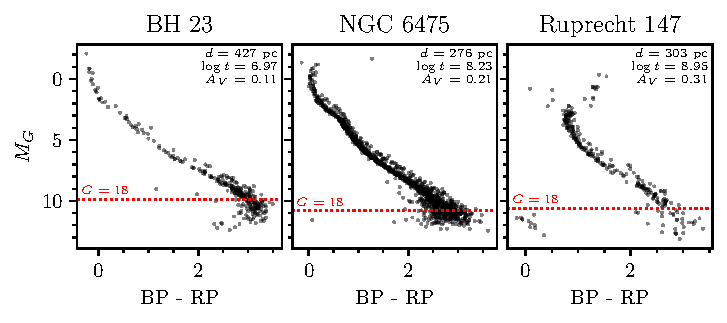
\includegraphics[width=\textwidth]{fig/c1/cmd_comparison.pdf}
	\caption[A comparison of the CMDs of a number of nearby OCs]{A comparison of the CMDs of a number of nearby OCs, using membership lists from later in this thesis in Sect.~\ref{sec:census} and plotted with their absolute magnitude $M_G$ against colour $BP - RP$. The OCs are plotted from left to right in order of increasing age, with their distance $d$, logarithmic age $\log t$ and extinction $A_V$ shown in the top right. The dashed red line indicates the approximate 100\% completeness limit of these OC membership lists, with sources fainter than an apparent magnitude of $G=18$ frequently being missed and often having under-estimated $BP-RP$ colours. BH~23 is less than 10~Myr old and has almost no main sequence turn off; NGC~6475 is over 100~Myr old and has a clear turn off; Ruprecht~147 is around 1~Gyr old and even has a clear population of white dwarf stars.}
	\label{fig:intro:history:cmds}
\end{figure}

The 20\textsuperscript{th} century saw improvements to data gathering and techniques, with early photometric and spectroscopic methods allowing authors such as \cite{rosenberg_uber_zusammenhang_1910} and \cite{hertzsprung_ueber_verwendung_1911} to plot the brightness of the stars in the Pleiades and the Hyades against their spectral features, noticing for the first time that the brightness of stars is related to their colour and spectral features. \cite{russell_relations_spectra_1914} derived the absolute magnitude of stars in the Hyades and ploted this against an early spectral analogue of the temperature of its member stars, plotting the luminosity of stars against their temperature for the first time and inventing `Hertzsprung-Russell' or `colour-magnitude' diagrams (CMDs), a type of plot used extensively in the present day as an essential tool to understand stellar evolution. Later, the differences in CMDs between different clusters were noticed and was interpreted as being a difference in age between the clusters, allowing for the ages of stars within star clusters to be estimated and beginning the foundation of our knowledge of stellar evolution \ref{fig:intro:history:cmds}.

While the 20\textsuperscript{th} century saw huge strides in our understanding of stars and star clusters, the size of OC catalogues went relatively unchanged (Fig.~\ref{fig:intro:history:catalogues}). It was not until the 1990s and the arrival of new methodologies that the OC census itself has begun its largest upheaval since the widespread adoptation of reflecting telescopes more than 200 years prior.


\subsection{The advent of modern astrometry and infra-red datasets}

The launch of the \emph{Hipparcos} satellite and subsequent data releases \citep{perryman_hipparcos_1997} produced a catalogue of around 10$^5$ sources with five-parameter milliarcsecond-precision astrometry. OCs stand out as overdensities in \emph{Hipparcos} data, in particular in proper motions, as OCs are comoving groups of stars that often have different velocities to background field sources. This new data allowed works such as \cite{platais_search_1998} to discover a number of new OCs, with many being small objects near to the Sun that evaded detection with only two-dimensional visual observations. 

This resulted in the catalogue of \cite{dias_new_2002} including over 300 more objects than the roughly ten years prior catalogue of \cite{mermilliod_database_1995} (Fig.~\ref{fig:intro:history:catalogues}), representing the largest 
major jump in the size of the OC census in over a century, in addition to the much more accurate mean cluster proper motions and parallaxes provided by \emph{Hipparcos}. However, this was just the beginning, and more new science was to come.

The release of the Two Micron All Sky Survey \citep[2MASS,][]{skrutskie_two_2006} in the 2000s provided the next major jump in data availability for furthering OC science. The infrared (IR) data of 2MASS and its associated catalogue of 471 million point sources allowed works such as \cite{froebrich_systematic_2007} to uncover over a thousand new OC candidates in the galactic disk, using IR data to peer through insterstellar dust and unveil many previously-obscured objects for the first time. In addition, works around this time began to make increasing use of advances in computing power, with works such as \cite{froebrich_systematic_2007} using automated retrieval to extract cluster candidates. CITEME MORE REFERENCES HERE

Work predominantly with IR data culminated in the catalogue of \cite{kharchenko_global_2013}, who derived homoegeneous membership lists, ages, extinctions, distances, proper motions, radii, and many other parameters for a total of 3006 clusters, 2399 of which are OCs or probable OCs. % Until \gaia\ DR2, the catalogue of \cite{kharchenko_global_2013} remained the largest catalogue of OCs.

In around 20 years, the OC census more than doubled in size between the work of \cite{mermilliod_database_1995} to the work of \cite{kharchenko_global_2013}. This unprecedented shift represented the first time that the OC census had been significantly expanded in over a century, with improved datasets offering significantly better measurements of more clusters than ever before. 

Yet the seismic shift in cluster catalogues brought about by IR datasets and \emph{Hipparcos} was scarcely the beginning of the modern revolution in studies of OCs. \gaia's first full data release in 2018, DR2 \citep{brown_gaia_2018}, sparked the next revolution in the census of OCs.


\section{The \gaia\ revolution}
\label{sec:intro:gaia}

For almost all of the history of astronomy, our view of the Milky Way has been strictly two-dimensional. Observing a three-dimensional galaxy in two dimensions is inherently limiting; it took until the 20\third\ century to even discover that galaxies are separate from the Milky Way CITEME. Although astrometric parameters like parallaxes have been measured for stars for over a century, and can be used to view the stars of the galaxy in three dimensions, these datasets have always been limited to a few hundred or thousand stars until very recently. % can I get PMs in here somehow?

\subsection{Background on the \gaia\ satellite}
\label{sec:intro:history:gaia:background}

\gaia\ is a space-based telescope launched in 2013 that aims to measure a wealth of parameters to an unprecedented level of precision for around $10^9$ stars. \gaia\ is measuring precise positions, proper motions, parallaxes, and photometry for its full sample of stars, and also measures radial velocities and low-resolution spectra for a brighter subsample of sources \citep{gaia_collaboration_gaia_2016}. It is the incredible scale and precision of \gaia\ data that sets it apart from any previous datasets.

% Plot of hipparcos vs. gaia astrometric accuracy
\begin{figure}[tb]
	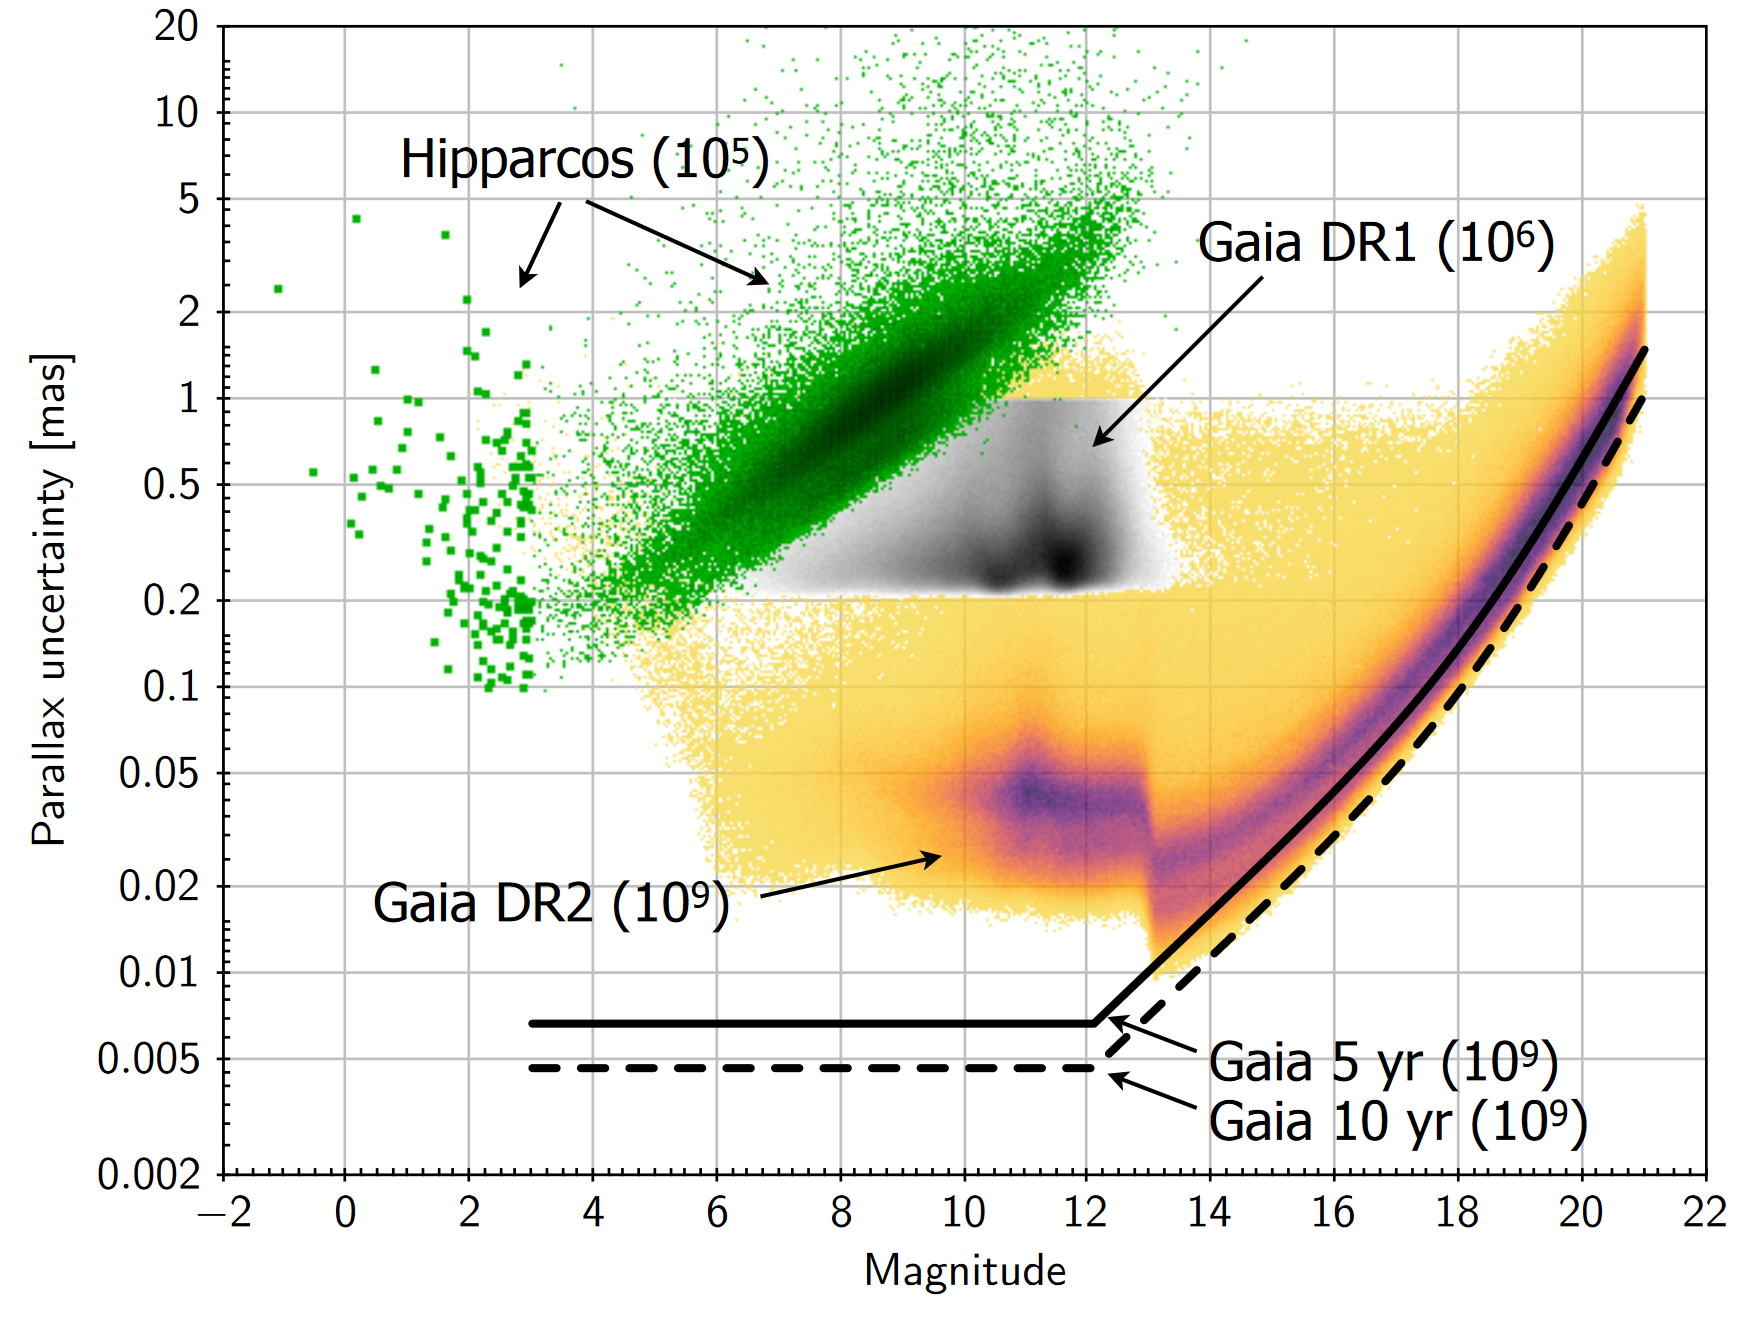
\includegraphics[width=\textwidth]{fig/c1/gaia_dr2_astrometry.png}
	\caption[Comparison between the astrometric accuracy for Hipparcos, Gaia, and future Gaia data releases]{Comparison between the astrometric accuracy for all sources in the final data release of Hipparcos, \gaia\ DR1, and \gaia\ DR2. The predicted accuracy of future data releases using 5 and 10 years of data is shown by the solid and dashed lines respectively. \emph{Credit}: \gaia\ DPAC.}
	\label{fig:intro:history:gaia_accuracy}
\end{figure}

Figure~\ref{fig:intro:history:gaia_accuracy} shows a comparison of the parallax uncertainty of \gaia\ data against data from the \emph{Hipparcos} satellite. The difference in accuracy and quantity of data is clear: \gaia\ can measure parallaxes for $10^4$ times as many stars at a projected eventual accuracy as much as $10^3$ times better than \emph{Hipparcos}. Inevitably, such a large increase in the amount (and quality) of data has huge implications for the study of all objects in the Milky Way, of course including OCs.

% Plot of gaia astrometric tracks
\begin{figure}[tb]
	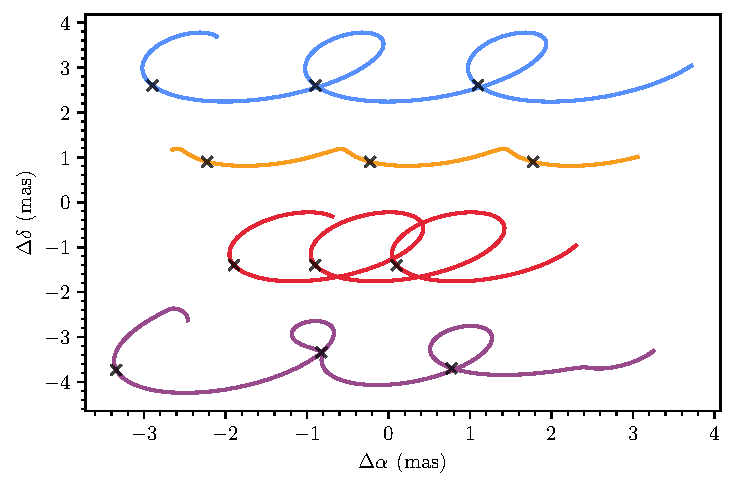
\includegraphics[width=\textwidth]{fig/c1/tracks.pdf}
	\caption[The predicted on-sky astrometric tracks of stars with different parameters]{The predicted on-sky astrometric tracks of stars with different parameters, generated using astromet \citep{penoyre_astrometric_2022}. All sources are at coordinates $\alpha,\,\beta=(0\degree,\,45\degree)$, but are offset in the $y$ direction for clarity of plotting. The first source has $\mu_{\alpha^*}=2$~masyr\textsuperscript{-1}, $\mu_{\delta}=0$, and is at a distance of 1~kpc. In the second example, the distance is quadrupled relative to the first. In the third example, the proper motion is halved relative to the first. In the final example, a binary with a period close to 1~yr, high eccentricity, and a low light ratio is added to the first example, producing a highly irregular track. The crosses denote the position of each source in one-year intervals.}
	\label{fig:intro:history:gaia_tracks}
\end{figure}

To truly understand the wonder of the \gaia\ satellite, it is first worth discussing how exactly it works. Although our galaxy is a dynamic system, with stars continually orbiting around the centre of the Milky Way \citep{binney_galactic_1987}, it is exceptionally difficult to capture the movement of our galaxy in real time. To the human eye, the night sky is static; even the closest stars with the highest proper motions and parallaxes have movements across the sky measured in arcseconds, with one arcsecond being equivalent to just $1/3600$ of a degree. For stars at a distance of, say, 1~kpc, their parallax will amount to just 1~mas. With the Milky Way having an estimated radius of around 25~kpc CITEME, it is clear that measuring precise astrometry for even a small fraction of the stars in the galaxy requires an incredible level of precision.

Using techniques originally pioneered with the \emph{Hipparcos} satellite, \gaia\ operates quite unconventionally relative to traditional `point and take a picture' telescopes. Instead, \gaia\ gathers data by rotating at a rate of exactly 1\textdegree\ per minute, spreading point sources into lines on its detector which are then processed into sources at a given location. Coupled with the field of view of the telescope, this scanning pattern means it visits every location on the celestial sphere around 14 times a year, allowing the complicated track of sources across the sky (particularly for binary stars) to be reconstructed to an exceptionally high level of precision for around 1~billion sources (see Fig.~\ref{fig:intro:history:gaia_tracks}). \gaia's controlled rate of rotation, its view of the cosmos undisturbed by atmospheric distortion, and its precise, modern detectors allow for \gaia's revolutionary measurements to be possible \citep{gaia_collaboration_gaia_2016}.


\subsection{The \gaia\ impact on the census of OCs}
\label{sec:intro:gaia:census}

% Plot of hipparcos vs. gaia Blanco 1
\begin{figure}[p]
	\centering
	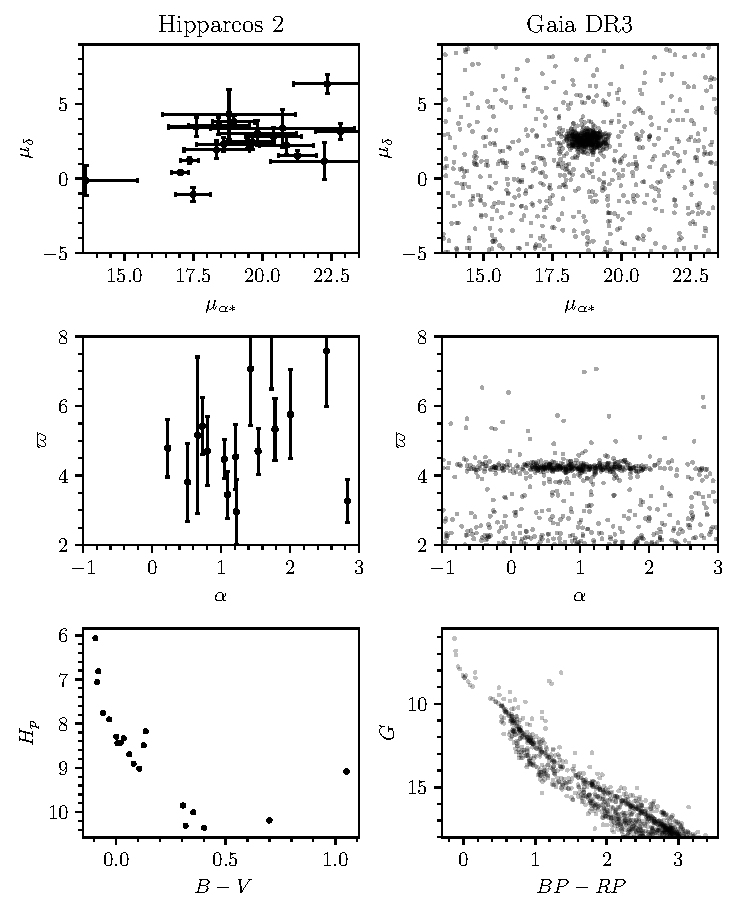
\includegraphics[width=\textwidth]{fig/c1/gaia_hipparcos_oc_comparison.pdf}
	\caption[Comparison between the regions around the star cluster Blanco~1 in data from \emph{Hipparcos} and \gaia]{Comparison between the regions around the star cluster Blanco~1 in data from \emph{Hipparcos} and \gaia. \emph{Hipparcos}-2 data \citep{vanleeuwen_hipparcos_new_2007} is shown on the left and \gaia\ DR3 data \citep{gaia_collaboration_gaia_2022} is shown on the right. The top row shows proper motions, the middle row shows parallax as a function of right ascension, and the bottom row shows the CMD of the stars in each region. While \emph{Hipparcos} only sees a few dozen bright stars for the cluster, \gaia\ can detect up to 1000, and to a significantly higher degree of astrometric accuracy.}
	\label{fig:intro:history:gaia_blanco_1}
\end{figure}

With so much data at an incredible level of quality, it is perhaps unsurprising that the OC census has been completely overhauled in just five years since the release of \gaia\ DR2. In many ways, \gaia\ is the perfect instrument for the study of OCs. Most OCs (such as NGC~2547 in Fig.~\ref{fig:intro:definition:comparison}) have relatively low star counts and are situated on the galactic disk, where high numbers of field stars are present -- making them challenging to isolate from background sources \citep{kharchenko_global_2012}. However, as OCs are comoving groups at a similar distance to one another and denser than the surrounding field, \gaia's proper motions and parallaxes provide an excellent way to isolate clusters from the field \citep{cantat-gaudin_characterising_2018}.

Figure~\ref{fig:intro:history:gaia_blanco_1} shows the region around the high galactic latitude OC Blanco~1 in data from the Hipparcos-2 catalogue \citep{vanleeuwen_hipparcos_new_2007}, compared against the same region in data from \gaia\ DR3 \citep{gaia_collaboration_gaia_2022}. The difference in precision between the two datasets is dramatic. In \emph{Hipparcos}, while the cluster is visible as an overdensity in proper motion space, in \gaia, the cluster becomes a small, compact group of stars that is trivially easy to separate from field stars. In addition, while Hipparcos parallaxes have accuracies on the order of 1~mas, \gaia\'s $\sim100\times$ better parallaxes make the cluster stand out as a clearly visible horizontal line as a function of right ascension. Combined together, proper motions and parallaxes make an exceptionally powerful tool to isolate OCs from field stars and derive clean, minimally contaminated membership lists. In addition, the difference in dataset size between the two telescopes is abundantly clear: \gaia\ DR3 can be used to probe the cluster eight to ten magnitudes fainter than \emph{Hipparcos}, resulting in a membership list around $\sim50\times$ larger than the cluster in \emph{Hipparcos} data. This incredible level of astrometric precision is repeated across the entire galactic disk, and has powered the last five years of revolution in the OC census.

% TODO: DR1? you may want to talk about DR1 tbh

Not long after the release of \gaia\ DR2, \cite{cantat-gaudin_gaia_2018} produced an updated catalogue of OCs and OC membership lists, using pre-\gaia\ works such as \cite{kharchenko_global_2013} as input and trying to redetect their catalogued clusters in \gaia\ data. \cite{cantat-gaudin_gaia_2018} were able to derive updated cluster membership lists with around twice as many members on average as in \cite{kharchenko_global_2013}, as well as deriving cluster proper motions to around two orders of magnitude greater precision than in \cite{kharchenko_global_2013} and precise distances to clusters.

One of the largest results of the work on the OC census so far in the era of \gaia\ has been that many clusters catalogued before \gaia\ cannot be detected in \gaia\ data. This is clear in Fig.~\ref{fig:intro:history:catalogues}, with the catalogue of \cite{cantat-gaudin_gaia_2018} containing around half as many clusters as \cite{kharchenko_global_2013}. The reasons for the non-detection of such a large number of OCs remain unclear. How can so many objects catalogued before \gaia\ be undetectable?

\cite{cantat-gaudin_clusters_2020} provided some answers to this question, searching again in \gaia\ DR2 data for many of the clusters they were unable to detect. They found that many clusters reported earlier in IR datasets continued to be undetectable in \emph{Gaia}, being able to strongly rule out 38 objects as definite asterisms. The asterisms they found are generally older and at high galactic latitudes, and were typically reported in IR datasets. They comment that although \gaia's visual observations should mean some clusters are too heavily reddened to be visible to \gaia, there are nevertheless many objects that \gaia\ should still be able to detect, owing to its deep visual photometry and ease of separating OCs from the field. However, the status of at least another $\sim$1000 clusters remains unknown, with the exact reasons for their non-detection in \emph{Gaia} being only speculation at this time. 


\subsection{New open clusters found with \gaia}
\label{sec:intro:gaia:new_clusters}

% Plot of reported OCs
\begin{figure}[tb]
	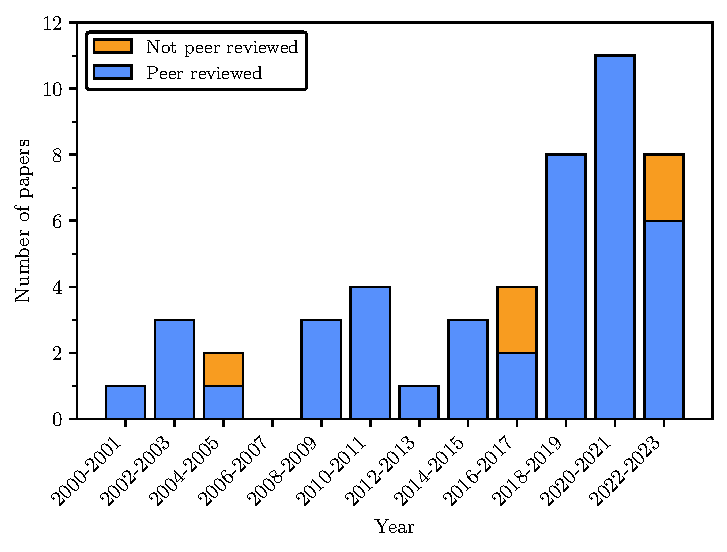
\includegraphics[width=\textwidth]{fig/c1/papers.pdf}
	\caption[The approximate number of papers reporting new open clusters in the 21\first\ century]{The approximate number of papers reporting new open clusters in the 21\first\ century, shown as a stacked bar chart of peer reviewed and non-peer reviewed works. Data for 2022-2023 are incomplete.}
	\label{fig:intro:history:papers}
\end{figure}

At the same time that \gaia\ has been an invaluable tool for better cataloguing already-known OCs, \gaia\ has also allowed for a large number of new OC discoveries; particularly for smaller, sparser objects that are otherwise impossible to find in 2D datasets \citep{cantat-gaudin_milky_2022}. Figure~\ref{fig:intro:history:papers} shows the approximate number of papers reporting new OCs in the 21\first\ century. Papers were found by searching the ADS\footnote{\url{https://ui.adsabs.harvard.edu/}} in Februrary 2023 for papers whose title or abstract contained the string `\texttt{new open cluster}'. The release of \gaia\ DR2 in 2018 \citep{brown_gaia_2018} clearly corresponds with the number of papers reporting new OCs each year roughly doubling.

The central challenge of finding new OCs in data from \gaia\ is the sheer size of the \gaia\ dataset, with hundreds of millions of stars to search through in a five-dimensional dataset of positions, proper motions and parallaxes for each star. While traditional approaches in the 19\third\ and 20\third\ centuries searched for clusters by hand, and works such as \cite{froebrich_systematic_2007} refined this approach by using kernel density estimation to identify overdense regions in the two-dimensional 2MASS dataset, the release of \gaia\ has also seen many new approaches for OC recovery.

Machine learning (ML) has exploded into observational astronomy over the last decade, developing from a niche method into a mainstay of observational methods CITEME. ML has two primary appeals. Firstly, it mostly automates the solving of complicated problems. ML can learn the relationship between input data and a desired output largely autonomously, with the user only being responsible for checking its work. Especially for arduous tasks like classification of large datasets \citep[e.g.][]{killestein_transient-optimised_2021}, ML-based approaches can be orders of magnitude more straightforward to implement than creating a brand new algorithm or approach to solve every problem every time, or by simply solving a problem by hand as would be done traditionally. In this way, ML methods can be considered a `Swiss army knife' of model fitting, with every method being applicable to a very wide range of potential problems. Secondly, ML-based approaches are generally much quicker than previous methodologies \citep{hunt_improving_2021}, leveraging the latest computing hardware such as graphics processing units (GPUs) significantly more efficiently than previous methods.

While ML is not without caveats which will be discussed at length later in this thesis, ML has still been essential to the dramatic increase in newly reported OCs in the \gaia\ era. \cite{castro-ginard_new_2018} were the first authors to adopt an ML-based approach for OC recovery, using two kinds of ML to automate tasks in cluster searches. Firstly, they used a clustering algorithm called DBSCAN (a form of unsupervised ML) to recover 31 new OCs in \gaia\ DR2 data, automating the process of cluster retrieval. Then, they used a neural network (a form of supervised ML) to classify OCs based on their CMD, also automating the process of assuring that OC CMDs have single stellar populations. Aside from \cite{sim_207_2019} and a handful of works where small numbers of new OCs were noticed by mistake \citep[e.g.][]{zari_3d_2018,bastian_gaia_2019,anders_ngc_2022-1}, all of the other roughly two dozen papers over the past few years that have found new OCs have used ML techniques to search for clusters.

Since then, many other works have used DBSCAN or variations on it to detect new clusters, with it proving to be an extremely popular method in the literature for OC retrieval \citep{castro-ginard_hunting_2019,castro-ginard_hunting_2020,castro-ginard_hunting_2022,liu_catalog_2019,he_catalogue_2021,he_new_2022,he_unveiling_hidden_2022,he_blind_allsky_2022,qin_discovery_2021,hao_sixteen_2020,hao_newly_2022,qin_hunting_2023}. In total, these works have reported nearly 4000 new OC candidates, which -- if all of these objects are real -- presents a major expansion in the size of the OC census. A handful of other works have used different methods, including \cite{cantat-gaudin_gaia_2019} who used Gaussian mixture models (GMMs) and \cite{jaehnig_membership_2021} who used extreme deconvolution (a probabilistic extension of GMMs).

The discovery of so many new OCs has brought a number of exciting new results. In particular, before \gaia, works such as \cite{kharchenko_global_2013} believed that the OC census of 955 objects was largely complete within 1.8~kpc; however, around $\sim$400 new OCs have been reported in this range by \gaia-based OC searches since the release of \gaia\ DR1, firmly challenging the idea that the OC census is complete at close distances and providing many new objects for study.

The most recent analysis of the completeness of the OC census in the \gaia\ era \citep{anders_milky_2020} found that the OC census within 2~kpc remains incomplete, although the full extent of this incompleteness is still an open question. It is unknown how many new OCs are remaining to be discovered and if existing methodologies could be improved upon.


\subsection{\gaia's brand new insights into open clusters}
\label{sec:intro:gaia:insights}

Although this thesis will mostly focus on methods to further improve the census of OCs, fundamentally, the reason why OCs are thoroughly important to modern observational astronomy is the science that can be performed with them. Hence, I will also quickly discuss some of the main new results into OCs that \gaia\ data has enabled, giving an overview of the power and importance of these objects.

% Plot of Meingast+ tidal tails/comas
\begin{figure}[tb]
	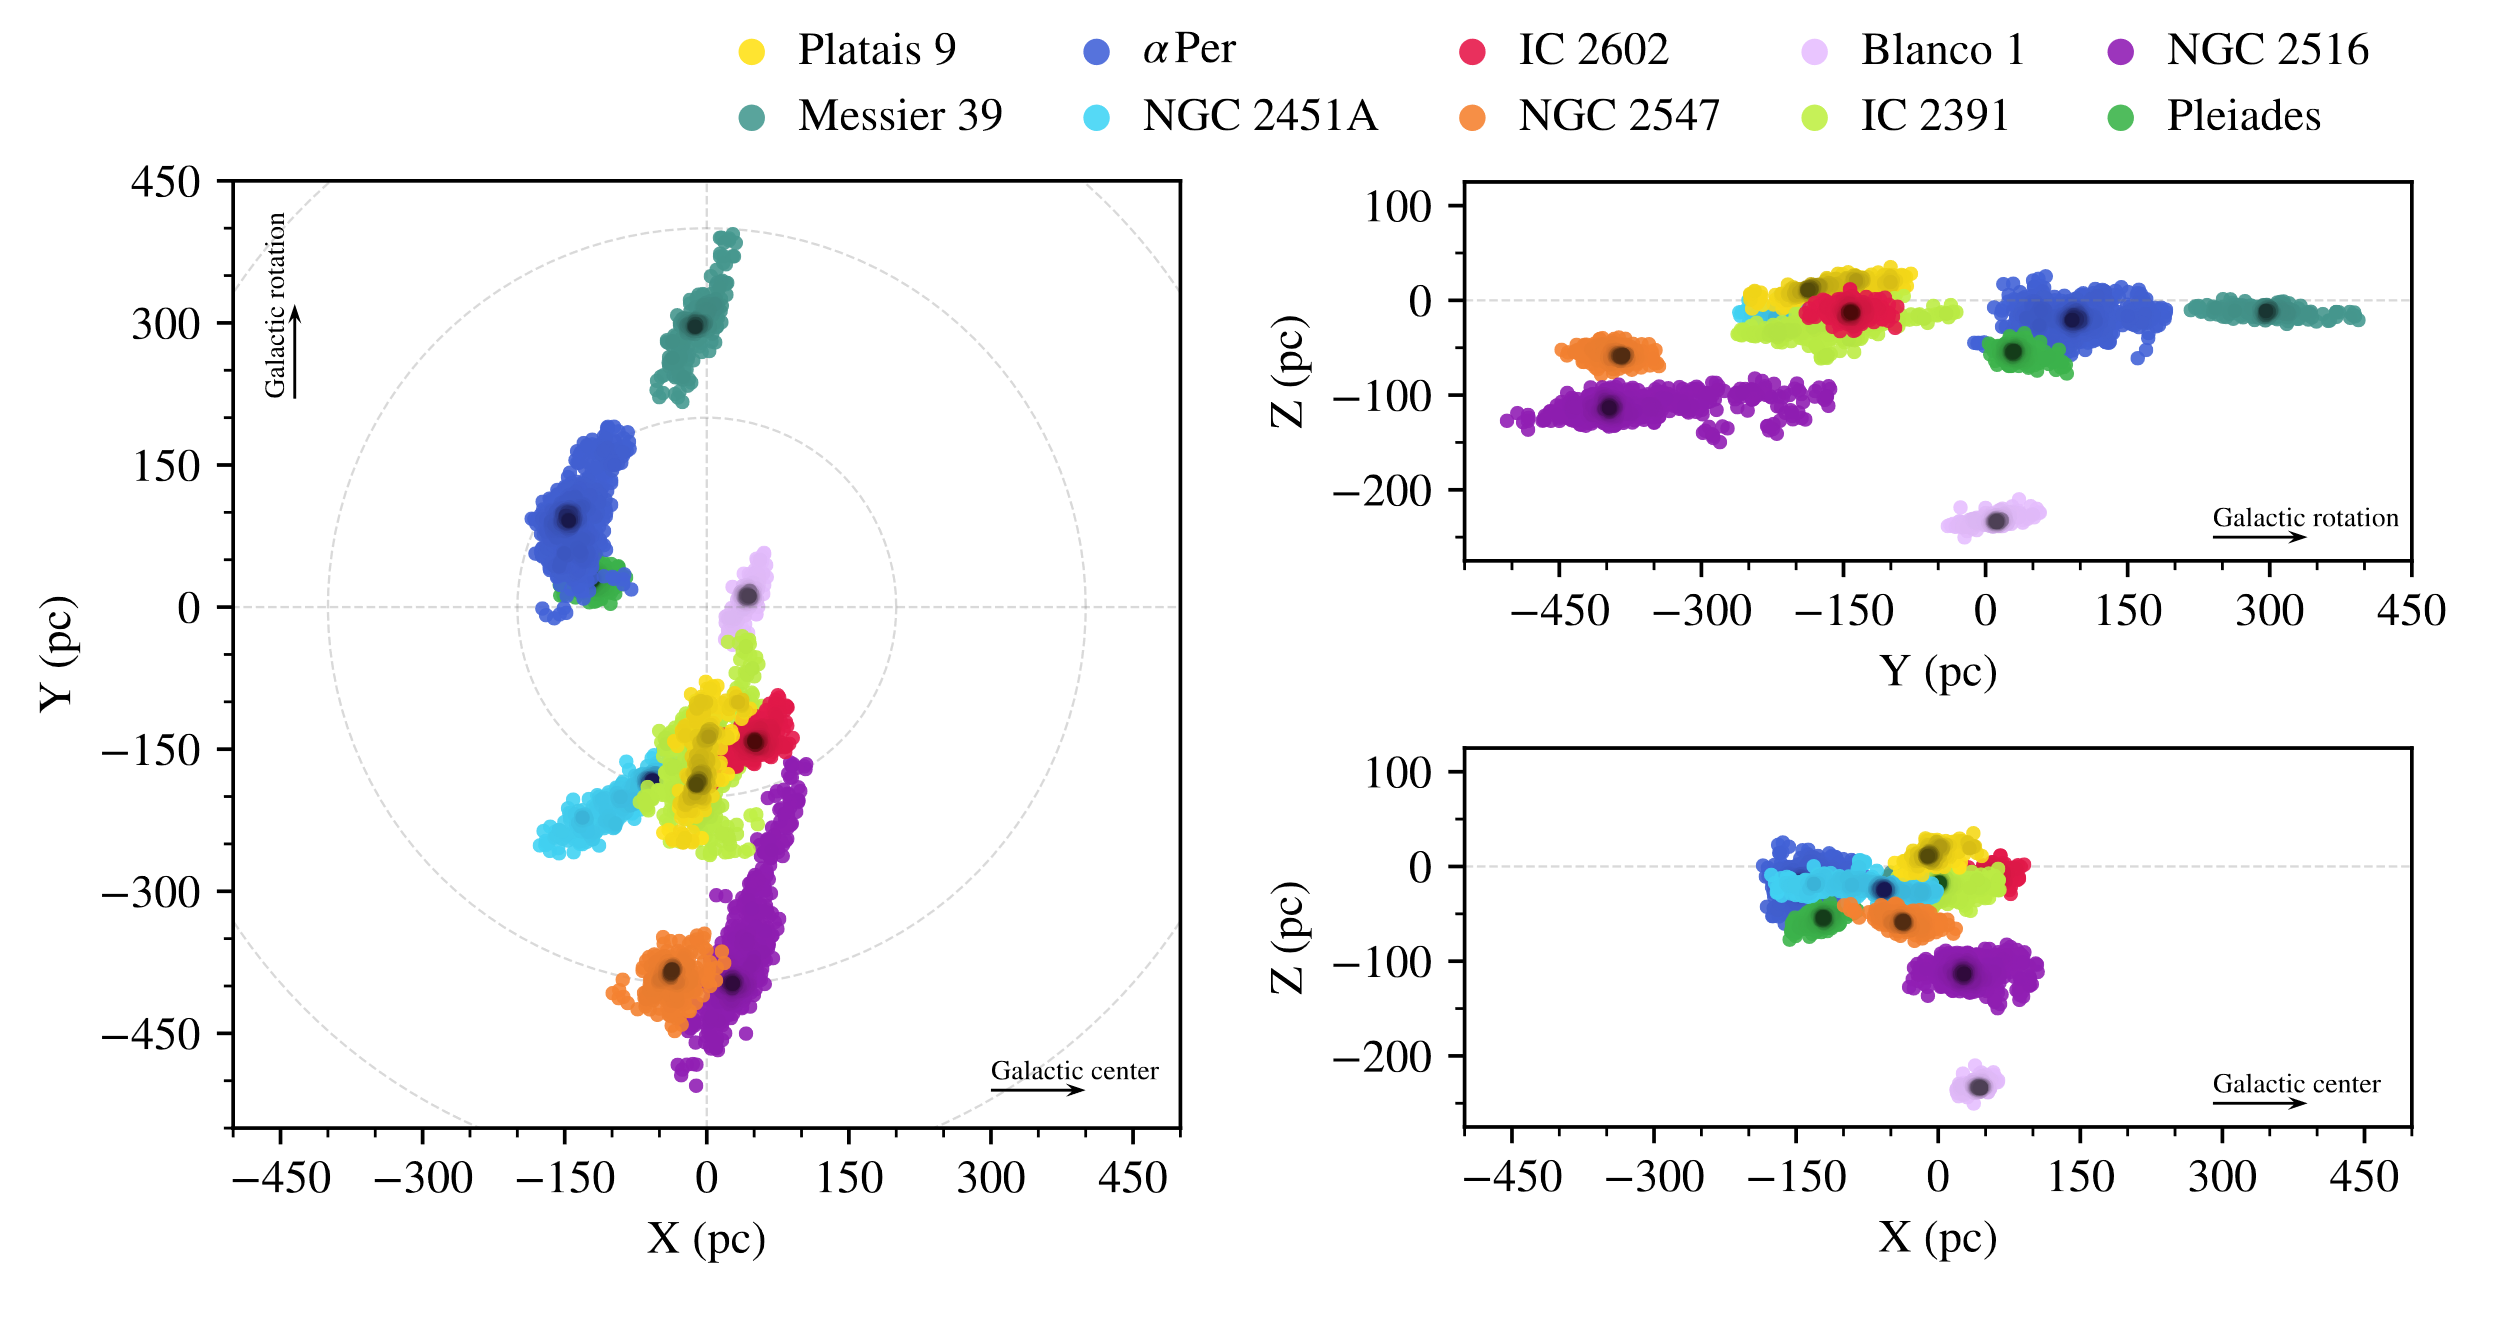
\includegraphics[width=\textwidth]{fig/c1/meingast_tidal_tails.png}
	\caption[The detected tidal tails and comas of ten OCs near to the Sun]{The detected tidal tails and comas of ten OCs near to the Sun. Clusters are shown as coloured density plots and plotted in heliocentric coordinates with the galactic centre to the right. \emph{Credit:} \cite{meingast_extended_2021}}
	\label{fig:intro:gaia:comas}
\end{figure}

One of the most exciting results of the \gaia\ era is that the dissolution of OCs can now be observed. OCs have a typical age of around 100~Myr, which is significantly younger than the $\approx 13$~Gyr age of the Milky Way, a difference that has long been argued as evidence that OCs are broken up by two-body interactions between stars ejecting some cluster members and the tidal forces of the Milky Way. Numerical simulations have shown that almost all OCs should have `tidal tails' of stars stretching in front and behind the cluster's orbit due to such interactions with the Milky Way's potential \citep{portegies_zwart_young_2010,cantat-gaudin_milky_2022}, although such tidal tails had only been observed for GCs until \gaia. Now, thanks to \gaia, the detection and study of OC tidal tails and dissolution processes is possible in exquisite detail for dozens of clusters.

As the nearest OC to the Sun, the Hyades has been extensively studied, with its spatial elongation first being probed by \cite{reino_gaia_study_2018} using \gaia\ DR1, and studied further by \cite{lodieu_3d_view_2019}, \cite{röser_hyades_tidal_2019}, and \cite{meingast_extended_stellar_2019}. Similar analyses have been performed on many more clusters, with \cite{meingast_extended_2021} analysing ten OCs in the solar neighbourhood and finding that not only do they all exhibit tidal tails, but most are also surrounded by `comas' of stars ejected in all directions from each cluster (Fig.~\ref{fig:intro:gaia:comas}). \cite{tarricq_structural_2022} studied 369 clusters within 1.5~kpc and detected tidal tails for 71 of them. Such clear visibility of the ongoing dynamical destruction of Milky Way OCs has been used by works such as \cite{yeh_ruprecht_2019}, \cite{oh_kinematic_modelling_2020} and \cite{pang_3d_2021} to study the dynamics of nearby OCs and make predictions on their future lifespan. It should be possible to expand these methods to more OCs and derive dynamical parameters for a wide range of star clusters, making wide-ranging inferences about the life of star clusters after their formation.

% Plot of OC spiral arm sort-of correlation
\begin{figure}[t]
	\centering
	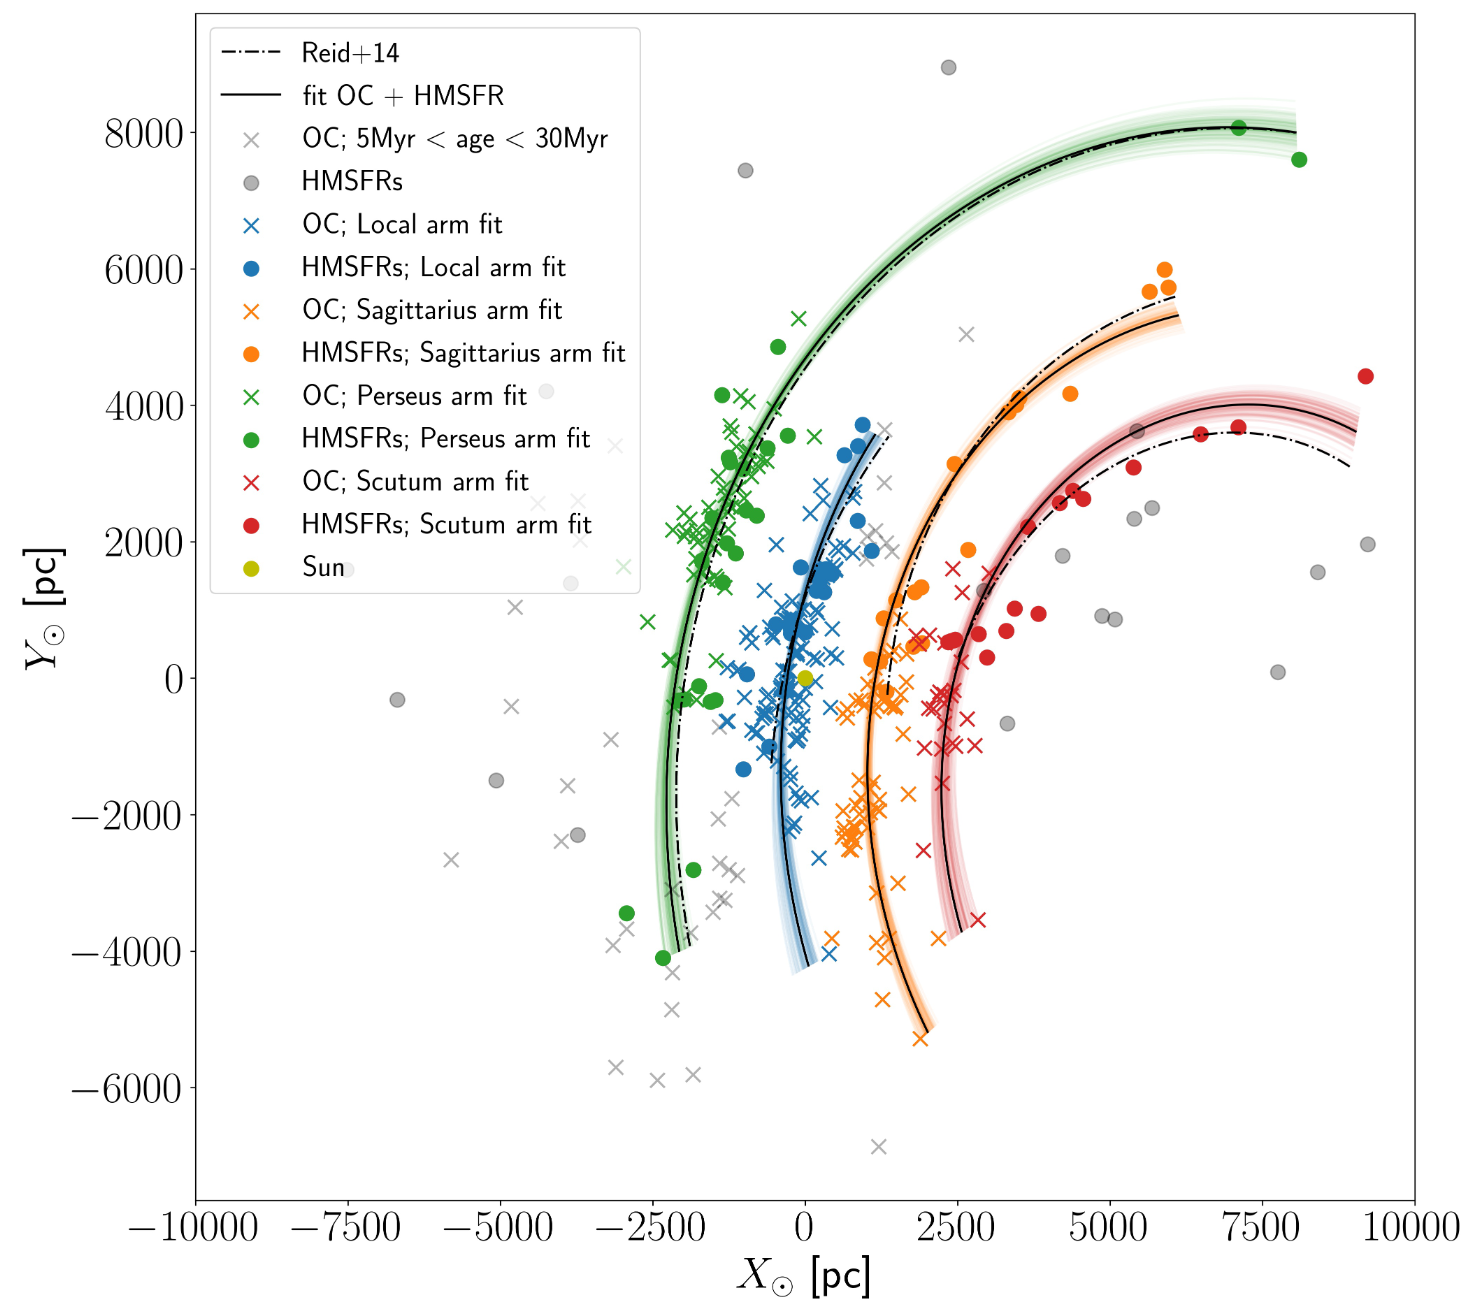
\includegraphics[width=0.8\textwidth]{fig/c1/spiral_arms.png}
	\caption[A model of the Milky Way's spiral arm structure as traced by OCs and high-mass star forming regions]{A model of the Milky Way's spiral arm structure as traced by OCs and high-mass star forming regions. \emph{Credit:} \cite{castro-ginard_milky_2021}}
	\label{fig:intro:gaia:spiral}
\end{figure}

OCs have also been extensively used to probe the wider structure of the Milky Way. \gaia's improved parallax accuracy allows for more accurate distances to OCs to be derived, and the improved OC membership lists possible with \gaia allow for better determination of photometric parameters. \cite{cantat-gaudin_painting_2020} derived ages, extinctions and distances for around 2000 OCs, showing that young clusters are generally correlated towards low galactic altitudes and appear to loosely trace spiral arm models derived from masers in works such as \cite{reid_trigonometric_parallaxes_2014}, while older clusters are more uniformly dispersed and can be found at higher altitudes above or below the galactic plane, suggesting that their orbits have evolved while they aged. \cite{castro-ginard_milky_2021} used these results to perform fits of a spiral arm model to a combination of the distribution of young OCs and star forming regions (Fig.~\ref{fig:intro:gaia:spiral}), finding that the addition of young OCs slightly changes the most likely spiral arm model relative to the fit of \cite{reid_trigonometric_parallaxes_2014}.

Finally, new OC results in the \gaia\ era have allowed for a number of new studies of stellar evolution. In particular, many more exotic phases of stellar evolution can now be studied more easily thanks to \gaia\ OC membership lists, which allow for significantly easier separation of OC member stars from field contamination. 

A primary hot topic within the literature is blue straggler stars (BSSs), which are stars near to the main sequence turn-off of a cluster that are bluer and brighter than would otherwise be expected (e.g. four stars to the upper left of the turnoff point of Ruprecht~147 in Fig.~\ref{fig:intro:history:cmds}). These stars are interesting cases of non-ideal stellar evolution, with leading theories stating that BSSs may be caused by mass transfer, dynamical mergers, or a combination of multiple processes \citep{boffin_ecology_2015}. While BSSs have been extensively investigated in GCs, \gaia\ has allowed for many new investigations of BSSs in OCs \citep{cantat-gaudin_milky_2022}, such as in \cite{rain_blue_2020} who investigated BSSs in Trumpler~5, Trumpler~20, and NGC~2477, or \cite{vaidya_blue_2020} who studied BSSs in a further seven OCs and found that BSSs are not mass-segregated in two of of the seven clusters they studied. \cite{leiner_census_blue_2021} investigated BSSs in 16 OCs and found that standard population synthesis techniques do not produce enough BSSs when compared to \gaia\ observations. They found that changes to assumptions about binary mass transfer somewhat rectify differences between observations and theoretical predictions, although they found that it still remains difficult to create the observed number of BSSs from current theories, suggesting that theories of BSS formation may require additional physics.

Another hot topic within stellar evolution that is more easily investigated within star clusters is extended main-sequence turnoffs (eMSTOs). Initially observed only in Magellanic cloud clusters \citep[e.g.][]{bastian_effect_stellar_2009}, \gaia's improved contrast between cluster and field stars has allowed for eMSTOs to be observed in a number of Milky Way OCs \cite{marino_discovery_2018}. eMSTOs challenge traditional theories of star formation for smaller clusters such as OCs as they could be explained by multiple stellar populations of a range of ages. On the other hand, simpler theories such as different rates of stellar rotation or even circumstellar dust are also competing theories to explain the existence of eMSTOs \citep{milone_multiple_2022,dantona_role_dust_2023}.

Finally, OCs have also been used to study and calibrate variable stars. In particular, Cepheid variable stars are a critical first rung on the cosmic distance ladder, useful for finding accurate distances galaxies within a few Mpc of the Milky Way. Currently, tension in the Hubble parameter $H_0$ could be explained in number of ways, ranging from the dominant $\Lambda$CDM cosmological model being wrong to simply being a miscalibration of one or more rungs on the cosmic distance ladder. Hence, in this context, accurate calibration and study of Cepheid variables is essential to ruling out or confirming issues with Cepheids as the source of any $H_0$ tension, a task that multiple authors have used OCs to aid in. \cite{breuval_milky_way_2020} used OCs hosting Cepheid variables to derive a new Cepheid period-luminosity relation (Leavitt law) and derive an updated value for $H_0$, finding that the Hubble constant could be revised to a lower value still in some tension with Planck CMB results \citep{planckcollaboration_planck_2018_2020} when using \gaia\ astrometry and Cepheid OC members. Works including \cite{medina_revisited_2021}, \cite{zhou_galactic_2021}, and \cite{hao_open_2022} have searched for more Cepheid variable stars within OCs to assist in the further study of Cepheids.

It goes without saying that all scientific use cases of OCs rely on the OC census being accurate, and are greatly improved by it being as complete as possible. Even though this review may have presented a `rosy-eyed' view of the status of OC science in the era of \gaia, there remain many issues with the current status of the OC census, with many unanswered questions and barriers to easier usability of OCs for science. In the next section, I will discuss some of these problems at length, and briefly introduce how I will try to solve some of them in the rest of this thesis.



\section{Issues and solutions for the open cluster census}
\label{sec:intro:aims}

As detailed in Sects.~\ref{sec:intro:pre-gaia} and \ref{sec:intro:gaia}, there has been a huge amount of recent scientific progress in the OC census and in the study of OCs as a whole. However, the \gaia\ era of OC science is still relatively new, with many more years of data releases being anticipated. Inevitably, this will allow for a huge range of new scientific studies into OCs \citep{gaia_collaboration_gaia_2022}. 

To maximise the scientific potential of OCs, it makes sense to improve the census of OCs as much as possible, as well as developing `future-proof' methodologies that can be applied to future \gaia\ data releases as well as the current ones. The issues with the census of OCs in the Milky Way can be divided into five broad topics that I will discuss next.


\subsection{The issues with the open cluster census}
\label{sec:intro:aims:issues}
\subsubsection{Problem 1. The methods used to detect open clusters (and their biases)}
\label{sec:intro:aims:issues:detection}

As mentioned in Sect.~\ref{sec:intro:gaia}, the \gaia\ mission has provided the OC community with a tremendous quantity of data. However, until now, many different works have tried many different approaches for OC recovery (both for recovery of existing clusters and for blind searches), with no direct comparison having been done between different approaches. Additionally, modern computer science is fast-paced, particularly in the field of machine learning. Many different approaches exist for clustering data, only a handful of which have been trialed for OC recovery \citep{xu_comprehensive_2015}, despite the fact that publically available open-source implementations of these algorithms are often available and ready to use \citep[e.g.][]{scikit-learn}.

This causes a number of problems. Primarily, it is unclear whether or not existing approaches are subject to biases. Particularly since almost all blind searches for OCs have used DBSCAN (Sect.~\ref{sec:intro:gaia:new_clusters}), it could be that a bias with the algorithm could prevent certain clusters from being detected depending on their age, distance, or other parameters, which may mean that a whole type of new OC has been as-yet undiscovered within \gaia\ data. There is no certainty that all OCs that \emph{can} be detected \emph{have} been detected with \gaia.

It is also unclear how many false positives current approaches produce. Most works do not include an estimate of how many of their reported clusters are real \citep[e.g.][]{castro-ginard_new_2018,liu_catalog_2019,he_catalogue_2021}. It is not known whether or not it is safe to assume that the results of a clustering algorithm can always be trusted, and it is not known whether certain algorithms are more or less trustworthy.

Additionally, there are many quirks with the usability of current approaches. For instance, the comprehensive DBSCAN-based works of \cite{castro-ginard_new_2018,castro-ginard_hunting_2019,castro-ginard_hunting_2020,castro-ginard_hunting_2022} have adopted a sky tiling scheme that requires a large number of algorithm re-runs, resulting in a method that must be applied on a supercomputer \citep{castro-ginard_hunting_2022}. It is not known whether a more efficient approach that requires fewer computational resources and is easier to repeat on future data releases is possible. This is a particular issue as future \gaia\ data releases are likely to contain higher numbers of reliable sources \citep{gaia_collaboration_gaia_2022}, meaning that current approaches will need to be ran on five to ten times as many sources\footnote{Calculated for \gaia\ DR3, which contains $\sim$250 million sources with $G\leq18$, which is a commonly adopted cut; however, the final \gaia\ data release is projected to contain at least 1 billion sources \citep{gaia_collaboration_gaia_2016}.}.


\subsubsection{Problem 2. The status of clusters discovered before \gaia}
\label{sec:intro:aims:issues:pre_gaia}

Of the many clusters discovered before \gaia, fewer than 50\% have so far been re-detected in \gaia\ data \citep{cantat-gaudin_gaia_2018,cantat-gaudin_clusters_2020}. The fact that so many objects are missing from \gaia-based OC studies could represent a total paradigm shift in the census of OCs in the Milky Way, or it could be indicative of the limitations of \gaia. For every cluster, there are two possibilities.

In the case that an object is real but cannot be detected in \gaia\ data, such as for heavily reddened clusters discovered using IR datasets that are obscured by dust in \gaia\ data \citep{cantat-gaudin_clusters_2020}, such an object would be a sign of the incompleteness of the \gaia\ OC census. If a significant number of IR clusters are in fact real, then to study all known OCs, it would be necessary to use both \gaia\ and IR datasets simultaneously.

On the other hand, it is also possible that such objects are not real. \gaia\ has significantly higher astrometric accuracy than all previous astrometric catalogues, and \gaia\ should be sensitive to a large number of real OCs, even for those with intermediate levels of reddening \citep{cantat-gaudin_clusters_2020}. 

While some studies have performed small investigations into clusters missing from \gaia\ on a case-by-case basis \citep[e.g.][]{cantat-gaudin_clusters_2020,piatti_catching_2023}, the status of most objects is still unknown. It should be possible to rule out many OCs reported previously in the literature given a large enough study. Alternatively, if \gaia\ is in fact a major limitation in recovering many OCs discovered before \gaia\ using IR datasets, then different datasets would need to be used to study such objects. This would also be a further strong science case for \gaia\ follow-up missions such as the proposed \emph{GaiaNIR} mission for near-infrared astrometry \citep{hobbs_gaianir_combining_2016}.


\subsubsection{Problem 3. The status of clusters discovered with \gaia}
\label{sec:intro:aims:issues:post_gaia}

At the same time as the aforementioned `re-detection crisis' of clusters reported before \gaia, thousands of new OC candidates have been reported in the literature. Most of these objects have not been independently verified \cite{cantat-gaudin_milky_2022}, meaning that a large number of objects exist in the literature and may be being used for studies of OCs and galactic structure but without knowing which objects are or are not real \citep[e.g.][]{anders_milky_2020,castro-ginard_milky_2021}. Given that so many clusters cannot be detected from recent works reporting new OCs before \gaia, with some works such as \citep{scholz_global_2015} having as many as 100\% of their clusters being impossible to redetect \citep{cantat-gaudin_gaia_2018}, it is not far-fetched to suggest that there can be reproducibility issues between different studies when reporting new objects. Hence, there is a need to independently verify new OC candidates reported recently using \gaia\ data, preferably also with an alternative methodology and an analysis of which objects are and are not real.

Additionally, it is also possible that some objects reported recently are duplicates. The large number of papers reporting new OCs since the release of \gaia\ DR2 (Fig.~\ref{fig:intro:history:papers}) can make the literature difficult to keep up with \citep{cantat-gaudin_milky_2022}. There is likely a need to verify that new cluster candidates are unique and have not been previously reported in the literature. For instance, during the writing of this thesis, \cite{chi_blind_search_2023} (accepted in ApJS) reported 1179 new OCs, which would represent a large increase in the number of newly discovered OCs in the \gaia\ era. However, many plots of their `new' clusters are clearly compatible with OCs previously reported in the literature (e.g. candidate 14677, which is Blanco~1). The existence of works containing duplicates `muddies the water' when attempting to use existing catalogues of OCs in combination with papers reporting new objects. There is a clear need to verify that newly reported OCs are real, unique clusters. 


\subsubsection{Problem 4. The completeness of the \gaia\ open cluster census}
\label{sec:intro:aims:issues:completeness}

Despite the publication of many works that have used \gaia\ data to report thousands of new OCs (Sect.~\ref{sec:intro:gaia:new_clusters}), it is still unclear how complete the \gaia\ census of OCs is. It is not clear how many objects are missing or if any further biases contribute to certain objects being missing. Beyond the widespread disproving of the result in \cite{kharchenko_global_2013} that the OC census is complete within 1.8~kpc, there has been little study in the \gaia\ era on the completeness of the OC census.

Nevertheless, the completeness of any catalogue, not least the OC census, is an interesting thing to know that would enable a large number of scientific studies. The study of star clusters in the Milky Way is unique in that we are able to study bound star clusters of significantly lower masses and luminosities than is possible in extragalactic studies \citep{portegies_zwart_young_2010}. While extragalactic astronomy is able to probe the occurence rates of massive, highly luminous clusters in a large number of galaxies, it is only in the Milky Way that study of low-mass objects is possible, due to their low luminosity. Milky Way OCs are hence an important calibration point for understanding star formation at lower mass ranges.

Given that the Milky Way's cluster age and mass functions are uniquely important in the general study of star clusters, it is vital that the completeness of the OC census can be well known. Although this has been attempted in \gaia\ data by \cite{anders_milky_2020}, who also derive a completeness estimate of the OC census, their work has two main limitations. Firstly, they used the blind searches of \cite{castro-ginard_new_2018,castro-ginard_hunting_2019,castro-ginard_hunting_2020} to calibrate their completeness function. However, it is not known if the DBSCAN algorithm used in these works has any biases that their completeness estimate would inherit (see Problem~1/Sect.~\ref{sec:intro:aims:issues:detection}). Secondly, they only create a selection function in terms of cluster age and distance. They expect that other parameters, such as cluster mass or size, could be major factors in the OC selection function. They were unable to include mass in their selection function due to the lack of cluster mass measurements in the \gaia\ era.

In addition, it is not clear how many more new OCs could be detected with future \gaia\ data releases. In theory, it should also be possible to extend such a prediction to other proposed surveys and instruments such as \emph{GaiaNIR} \citep{hobbs_gaianir_combining_2016}. Given that the proposals for \emph{GaiaNIR} describe science with OCs as a key scientific justification for the mission, a way to predict how many OCs would be discovered by a near-infrared astrometric mission such as \emph{GaiaNIR} would be an interesting way to strengthen the science case for future astrometric missions and surveys.


\subsubsection{Problem 5. The observational definition of open clusters}
\label{sec:intro:aims:issues:definition}

Finally, and somewhat amusingly, possibly the greatest issue with the OC census in the \gaia\ era is that no work can agree on what OCs actually are (at least observationally). While the theoretical definitions of star clusters in the Milky Way can now be reasonably clearly defined \citep[Sect.~\ref{sec:intro:definition}][]{portegies_zwart_young_2010}, it is challenging to convert these theoretical definitions into a firm observational definition for OCs. Critically, this presents a number of issues when comparing between different works or when trying to combine the results of separate OC studies.

Most works reporting new OCs use different quality criteria to decide which objects are or are not included in their work. Almost all use some sort of criteria on colour-magnitude diagrams, requiring that the cluster CMD is narrow and compatible with a single stellar population. However, this is implemented in many different ways; including by using statistical criteria \citep[e.g.][]{liu_catalog_2019}, a neural network classifier \citep[e.g.][]{castro-ginard_new_2018}, or simple manual classification \citep[e.g.][]{he_catalogue_2021}. Some works require that clusters are clear statistical overdensities in \gaia, deriving something analogous to a signal to noise ratio (S/N) for their cluster candidates \citep[e.g.][]{cantat-gaudin_gaia_2019}. Some works also limit clusters based on their physical parameters, requiring that they are compact groups and hence more likely to be gravitationally bound \citep[e.g.][]{liu_catalog_2019}. Finally, all works adopt a different minimum size for an OC, ranging from as low as 8 stars \citep{castro-ginard_new_2018} to as high as 50 \citep{liu_catalog_2019}. With so many differing definitions of what constitutes a good enough OC candidate, it can be difficult to compare the results of multiple works or to combine them into singular catalogues without introducing biases. In addition, most works use simple binary `yes/no' cuts on whether or not an OC passes a given constraint, which may not capture all of the uncertainty inherent in deciding whether an edge-case object is or is not a real OC.

\cite{cantat-gaudin_clusters_2020} outlined a set of empirical criteria to follow that all new OC candidates should meet, requiring that OCs are a clear overdensity in astrometric data, that they have a CMD with a clear homoegeneous population of stars, and that the cluster meets two cuts on its parameters intended to be an analogous test for being bound: that the radius containing 50\% of members is smaller than 20~pc, and that the cluster's proper motion dispersion corresponds to an internal velocity dispersion of less than 5~kms\textsuperscript{-1}. While these criteria are an empirical minimum for an OC, as a thought experiment, it is still relatively straightforward in a dense region of the galactic disk to find $\sim$10 or more stars within 50~pc of each other and with a velocity dispersion below 5~kms\textsuperscript{-1}, and so these criteria are not infallible, and could allow unbound moving groups to be misclassified as OCs.

A `gold standard' observational definition of an OC might be more directly derived from the theoretical definition presented in Sect.~\ref{sec:intro:definition} -- requiring that an OC is an overdensity, a single stellar population, and gravitationally bound. However, no such way to transform observations into such a definition currently exists, principally due to the difficulty in measuring the dynamics and boundness of a large catalogue of star clusters.


\subsection{The aims of this thesis}
\label{sec:intro:issues:aims}

Even relative to the major improvements to OC science in the 1990s and 2000s, \gaia\ has still been utterly groundbreaking in the quality and quantity of data it provides on our galaxy. Never before has so much precise data been available for so many stars; \gaia\ will rewrite textbooks on the composition and characteristics of the Milky Way. Within the field of OCs, this is clear from the many incredible new \gaia\ results highlighted in Sect.~\ref{sec:intro:gaia}. Yet as the many problems discussed in the previous section show, many issues remain with the census of OCs. In this thesis, I hope to showcase timely research that can present solutions or partial solutions to the above problems, developing the methods used to analyse OCs in the \gaia\ era to maximise the scientific potential of these objects.

First and foremost, it is impossible to solve many of the other issues in the OC census without an understanding of the limitations and biases inherent to different methods for OC retrieval (Problem 1). In addition, numerous unexplored methods for cluster retrieval present in the computer science literature could provide better options for the recovery of OCs \citep{xu_comprehensive_2015}. To date, there has been no comparative study into the advantages and disadvantages of different approaches for cluster retrieval, despite the clear importance of understanding the limitations of different methods; hence, the first part of this thesis focuses on trialing different algorithms for OC recovery in \gaia\ DR2 data, performing a comparative study into their effectiveness. In this study, I will also aim to find optimal ways to divide \gaia\ data for OC retrieval, aiming to present a method that can be ran efficiently even on larger datasets, allowing for more sources to be incorporated in the future as \gaia\ data releases improve. In the best case scenario, a method can be found that can redetect the clusters reported by all other works with minimal bias.

With a best method found, other problems in the census will be more straightforward to solve. Finding the best methodology for OC retrieval and knowing its biases will allow for the application of the method to solve Problems 2 and 3, and to a lesser extent Problem 4. Specifically, in the second study of this thesis, I conduct a large-scale unbiased blind search for OCs using the best method found and data from \gaia\ (E)DR3. Depending on which \gaia-discovered clusters can be found in this search and depending on the effectiveness of the method found in the first study, it will be relatively simple to solve Problem 3, as some clusters will (or will not) be possible to re-detect. This study will conduct the largest validation of OCs discovered using \gaia\ to date.

An unbiased all-sky search will also allow for a solution to Problem 2. Previously, studies have generally focused on small, case-by-case attempts to retrieve OCs that were originally catalogued in pre-\gaia\ works \citep[e.g.][]{cantat-gaudin_clusters_2020}. However, an all-sky search ought to recover all OCs visible in \gaia\ within the limitations of the adopted methodology; given the understanding of this methodology gained from the first study, it should be possible to say with reasonable certainty whether or not \gaia\ should be able to detect many of the as-yet undetected OCs from before \gaia. This will greatly aid in bridging the OC census from pre-\gaia\ works to the \gaia\ era, tracing down any remaining missing clusters while suggesting that some are not real.

Inferring the completeness of the OC census is a major task, which this thesis will contribute towards but may not completely solve. An unbiased all-sky blind search for OCs is a good tool to find as many OCs as possible and reduce the incompleteness of the OC census. Despite the many works that have already searched for new OCs (Sect.~\ref{sec:intro:gaia:new_clusters}), there may still be many new objects left to discover. This search can be used as a drop-in replacement for the methodology of e.g. \cite{anders_milky_2020}, serving as a better `experiment' to detect a large sample of OCs. However, given that cluster masses are expected to be a major contributor to the selection function of OCs in \gaia, with less massive clusters being more difficult to detect, it will also be important to calculate accurate cluster masses for the entire sample of objects from the blind search. The final study of this thesis partly focuses on calculating cluster masses, which will help to solve Problem 4 while also deriving a generally useful parameter for OCs that has never been derived for such a large catalogue before. Cluster masses also require cluster ages, which I aim to derive estimates of in the second study to accompany the overall OC catalogue.

Finally, Problem 5 is likely to continue to plague the OC community for years to come, owing to the complexity of precisely defining OCs observationally. However, throughout this thesis, I will present new methods to try and convert a theoretical, first-principles oriented definition of an open cluster into a practical observational method to classify objects as OCs, MGs, GCs, false positives, or somewhere inbetween one of those categories. I aim to do so statistically, never presenting simple binary probabilities of an object being a false positive or one of the classes of real star cluster, but rather using a statistical treatment to aid in the definition of edge-case objects that could be between different classes. In the first study of this thesis, I augment clustering algorithms by trialing a number of different tests for the density of a cluster compared to its field, deriving a simple and efficient test of a cluster's astrometric signal to noise in \gaia\ data. In the second study of this thesis, I use an approximately Bayesian neural network to classify the likelihood of an OC being compatible with a single stellar population given the predictions of stellar evolution models. In the final study of this thesis, I present a preliminary method to test the boundness of OC candidates and ascertain if they are a real bound object or simply an MG.

In total, with this thesis, I hope to contribute to the difficult task of cataloguing and characterising the OCs of the Milky Way in the era of \gaia. Implicitly, all of these methods will be `future-proof' and applicable to future \gaia\ data releases, or future surveys that could replace the \gaia\ telescope. Inevitably, no method is perfect, and I will conclude by speculating on future avenues of research that could further develop the methods used to analyse OCs.


Before launching into the scientific content of this thesis, it is important to also present some theoretical background into OCs.


% ---------------------------------------
\section{Further background into star clusters and associated common methods}
\label{sec:intro:theory}

To improve the reach and readability of this thesis, I feel it is important to review some common techniques and pieces of theory from the literature. For the seasoned open cluster astronomer, this section could be browsed quickly; for the non-specialist, I hope that this section provides more insight into pieces of theoretical knowledge that I will assume for the scientific parts of this thesis.

I begin by going into more depth on some of the most important methods to OC observers.


\subsection{Analysis of CMDs}
\label{sec:intro:theory:cmds}

% Plot of CMDs of OCs
\begin{figure}[tb]
	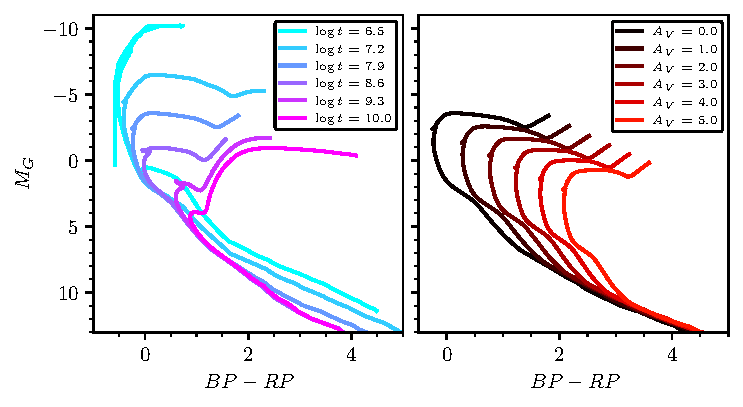
\includegraphics[width=\textwidth]{fig/c1/isochrones.pdf}
	\caption[A comparison between stellar isochrones of various different parameters.]{A comparison between stellar isochrones of various different parameters, derived from PARSEC stellar evolution models \citep{bressan_parsec_2012} and shown in \gaia\ photometric bands. \emph{Left:} isochrones of solar metallicity and zero extinction shown for six different ages. Most noticeably, as cluster age increases, the magnitude of the turn-off point decreases, with ever-more stars evolving into red giants and eventually reaching the end of their lives. The rest of the stars in the cluster also move down slightly, relaxing onto the main sequence as they age. \emph{Right:} the $\log t = 7.9$ isochrone from the left plotted at a range of different extinction values. Extinction reddens cluster stars as well as reducing their overall brightness. Extinction in \gaia\ photometry has a strong affect on the location of the turn-off point.}
	\label{fig:intro:history:isochrones}
\end{figure}

As discussed previously, CMDs are essential tools to derive many key parameters of a star cluster (Fig.~\ref{fig:intro:history:cmds}). The most common method to determine the age, extinction, and to a lesser extent the distance of a cluster is by fitting isochrones to cluster CMDs. An isochrone gives the predicted colour and luminosity of a population of stars with a range of masses given that the stars have the same age, extinction, composition and distance. Stellar isochrones are derived from stellar evolution models such as PARSEC \citep{bressan_parsec_2012} and are widely used in many areas of observational astronomy.

In practice, isochrones are difficult to fit, with age, extinction, distance and metallicity all being somewhat degenerate with one another. Figure~\ref{fig:intro:history:isochrones} shows the effect of varying age and extinction on stellar isochrones, with both age and extinction moving the location of the cluster turn-off point. Cluster distance merely shifts the isochrone up or down based on the cluster's distance modulus, although this is still slightly degenerate with age and extinction. Finally, the chemical composition of a cluster (most often parameterised with its metallicity $\left[\text{Fe}/\text{H}\right]$) has the smallest impact on cluster isochrones and is not shown, but will nevertheless slightly impact age and extinction determination.

Isochrone fitting is further complicated by the presence of other cluster features, such as the presence of a binary sequence due to unresolved binaries (see binary sequences in Fig~\ref{fig:intro:history:cmds}, showing a clear second line of stars sat slightly above the main cluster population).

Probably unsurprisingly, there are hence many methods used in the literature to fit isochrones to data. Particularly as computational power is a major hindrance to performing three or four-parameter fits with stellar isochrones, it was common to simply fit isochrones by hand (CITEME SOME EXAMPLES), which includes no robust uncertainty estimate and can open the door to human biases. The isochrones in \cite{kharchenko_global_2013} were fit using a hybrid method, with the authors fitting distances manually but then using $\chi^2$ minimisation to fit cluster age and reddening values. \cite{yen_reanalysis_2018} developed this methodology further to perform $\chi^2$ fitting of all cluster parameters. Finally, \cite{hippel_inverting_2006} created a full Bayesian methodology to fit isochrones to cluster CMDs, which is still used by works today in the \gaia\ era such as \cite{bossini_age_2019}.

By far the main flaw of cluster isochrone fitting is speed. Three or four-parameter fits using complicated stellar isochrones simply cannot be performed quickly, requiring significant amounts of computation time to complete in e.g. \cite{yen_reanalysis_2018}, making these key cluster parameters relatively time-intensive to derive using traditional isochrone fitting techniques. Alternatively, a recently developed approach used in \cite{cantat-gaudin_painting_2020} and \cite{kounkel_untangling_2020} uses neural networks trained on the results of a small subsample of precise isochrone fitting results for OCs to derive ages, extinctions and distances to clusters with significantly less computational time, although this approach has the disadvantage of first requiring that isochrone fits are available to use as a training dataset.


\subsection{Radial profiles}
\label{sec:intro:theory:profile}

The physical size of OCs is another important property that can be measured. The size of observed clusters can be compared against theoretical predictions, and interesting relationships between parameters such as the size of clusters as a function of their age can be determined \citep{tarricq_structural_2022}.

The simplest commonly used measure of the size of an open cluster is the radius containing 50\% of members, $r_{50}$, which is the median radius of all detected member stars from the cluster centre. This radius has been commonly measured in the literature for OCs \citep[e.g.][]{cantat-gaudin_gaia_2018,cantat-gaudin_clusters_2020}. For a cluster where the mass of member stars is not correlated with their position in the cluster, such that high and low mass stars are equally distributed throughout the cluster (i.e., the cluster is not mass segregated), $r_{50}$ is equivalent to a common theoretical definition -- the half-mass radius $r_{hm}$, a radius commonly measured in theoretical works due to its use in various dynamical equations \citep{portegies_zwart_young_2010}.

However, simple measures of cluster radius are not informative about the shape of a cluster, as clusters have long been known to have different shapes, with some clusters being more centrally concentrated in their `core' and others being sparser. It is helpful to apply models to OC radial profiles, allowing for the shape of clusters to be compared given models of a small number of parameters.

\citep{king_structure_star_1962} models are the most common models applied to star clusters. While originally derived for globular clusters, these models have also been shown to be a good fit to many OCs \citep[e.g. in ][]{piskunov_towards_2007}, with a radial distribution function $f$ given by:

\begin{equation}
	f = k \left\{ \frac{1}{\sqrt{1 + \left(r/r_c\right)^2}} - \frac{1}{\sqrt{1 + \left(r_t/r_c\right)^2}} \right\}^2
\end{equation}

\noindent
where $r$ is the distance from the cluster centre, $r_c$ is the radius of the core of the cluster (the radius at which the surface density drops to half that of the centre), and $r_t$ is the tidal radius of the cluster beyond which the Milky Way's potential is dominant. This can also be convenient to express in terms of the total number of stars within a distance $r$ from the center of a cluster $n(x)$, which is given by:

\begin{equation}
	n(x) = \pi r_c^2 k \left[ \ln(1+x) - 4 \frac{\sqrt{1+x} - 1}{\sqrt{1 + x_t}} + \frac{x}{1 + x_t} \right]
\end{equation}

\noindent
where $x = (r / r_c)^2$ and $x_t = (r_t / r_c)^2$.

As an empirical model, the \cite{king_structure_star_1962} model is mostly useful for simple observational comparisons between clusters, such as comparisons between the core and tidal radii between clusters of different ages \citep{kharchenko_global_2013,tarricq_structural_2022}. \cite{king_structure_1966} re-derives a similar model from theoretical principles, including by assuming that the velocity distribution of stars in the centre of a star cluster is isothermal and that the cluster is in virial equilibrium. The shape of these models is parameterised by a dimensionless variable $W_0$ which parameterises the concentration of a cluster, with higher values corresponding to a more centrally concentrated cluster. For $W_0 \lesssim 7$, \cite{king_structure_star_1962} and \cite{king_structure_1966} models are very similar. In practice, almost all OCs have $W_0 < 7$, and so these models can be used somewhat interchangeably \citep{portegies_zwart_young_2010}. Due to the significantly simpler functional form of \cite{king_structure_star_1962} models, they are used almost exclusively in the OC literature relative to \cite{king_structure_1966} models \citep{portegies_zwart_young_2010,cantat-gaudin_milky_2022}.

Finally, it is worth mentioning the model of \cite{plummer_problem_1911}. Once again originally designed for GCs, this model parameterises how centrally concentrated a star cluster is based on a single scale factor $a$. Unlike \cite{king_structure_star_1962,king_structure_1966} models, the \cite{plummer_problem_1911} model assumes star clusters do not have a physical limiting radius and extend to infinity, which is of course unrealistic. Nevertheless, the \cite{plummer_problem_1911} model is still a satisfactory approximation of star cluster distribution functions, and it is still used in the literature due to its simple functional form which can be solved analytically \citep{dejonghe_completely_analytical_1987}. \cite{plummer_problem_1911} models are particularly popular in theoretical studies of star clusters due to this reason \citep{portegies_zwart_young_2010}.


\subsection{Dynamics}
\label{sec:intro:theory:dynamics}

Later in this thesis, I use measures of OC dynamics to test if OCs are bound. Some works such as \cite{bravi_gaia-eso_2018} and \cite{pang_3d_2021} have used similar methods on small scales to test if OCs are bound. The following useful definitions are all from \cite{portegies_zwart_young_2010}.

Firstly, for a cluster with a one-dimensional velocity dispersion $\sigma_\text{1D}$, its total kinetic energy $T$ is approximately

\begin{equation}
	T = \frac{3}{2} M \sigma_\text{1D}^2
\end{equation}

\noindent
where $M$ is the total cluster mass. In addition, one can define the total potential energy of a cluster $U$ as 

\begin{equation}
	U = - \frac{GM^2}{2r_\text{vir}}
\end{equation}

\noindent
where $G$ is the gravitational constant and $r_\text{vir}$ is the theoretically definied virial radius of the cluster, a parameter that is difficult to calculate observationally as it requires three-dimensional positions. In practice, the virial radius can be defined as 

\begin{equation}
	r_\text{vir} = \frac{\eta}{6} r_{50}
\end{equation}

\noindent
where $\eta$ is a constant that is model-dependent. For an ideal \cite{plummer_problem_1911} model, $\eta$ is equal to 9.75, although in practice, this value can be out by a factor of two to four in extreme cases of star clusters with distributions that are poorly described by a \cite{plummer_problem_1911} model \citep{portegies_zwart_young_2010}.

Finally, putting these together, one can define the virial ratio $Q$ of a cluster, which is the ratio of kinetic to potential energy for a given bound system. Since the virial theorem predicts that $2T + U = 0$, $Q$ is hence given by

\begin{equation}
	Q = \frac{T}{\left| U \right|}
	  = \frac{\eta r_{50} \sigma_\text{1D}^2}{2GM}
	  \approx \frac{1}{2} \quad \text{for a bound cluster.}
	\label{eqn:intro:virial_ratio}
\end{equation}

\noindent
Equation~\ref{eqn:intro:virial_ratio} is also commonly expressed in terms of the predicted one-dimensional velocity dispersion of a virialised cluster $\sigma_\text{vir}$ \citep[e.g. in][]{bravi_gaia-eso_2018} as

\begin{equation}
	\sigma_\text{vir} = \sqrt{\frac{GM}{\eta r_{50}}}.
	\label{eqn:intro:virial_velocity}
\end{equation}

With these equations and measures of cluster mass, radius, and velocity dispersion, it is possible to probe the overall dynamical state of a cluster observationally or in the result of simulations \citep{banerjee_how_2017,bravi_gaia-eso_2018,pang_3d_2021}.


% \subsection{Timescales}
% \label{sec:intro:theory:timescales}

\subsection{Formation, evolution and destruction}
\label{sec:intro:theory:evolution}

Finally, having considered various individual pieces of important theory, it is also worth discussing the current overall theory of star cluster formation and evolution, which should give some theoretical context to the clusters observed at different ages in this work.


\subsubsection{Formation (up to \textasciitilde1 Myr)}

As discussed previously, stars form when clouds of cold molecular gas (giant molecular clouds, GMCs) within galaxies collapse due to gravity. This process is not believed or observed to be continuous: stellar winds from young stars rapidly heat and blow away any remaining gas within the cluster, preventing further star formation from occuring. Effectively, this process `freezes' star formation, ensuring that the resulting group of stars is roughly homogeneous in age and chemical composition \citep{lada_embedded_2003,krumholz_how_2020}. If the parent GMC is dense enough, then the stars will eventually collapse into a bound star cluster \citep{portegies_zwart_young_2010,krumholz_star_2019,krumholz_how_2020}. GMCs in the local universe generally have masses in the range $\sim10^3$ to $\sim10^7$~\MSun \citep{krause_physics_2020}. For exceptionally large GMCs with masses in excess of $\sim10^8$~\MSun, it is believed that they are large enough to form clusters as massive as GCs. Such conditions are rare in the current universe, being much more common at redshifts $z \gtrsim 2$ \citep{krumholz_star_2019}; such high-mass GMCs and the clusters they form are hence outside of the range of open clusters in this study, which generally have ages of no more than $\sim$1~Gyr. 

Historically, it was believed that all stars formed in bound star clusters. However, recent observations with \gaia\ have suggested that it may only be a minority of stars that form in bound clusters \citep{ward_not_2019,wright_ob_associations_2020}. Nevertheless, for GMCs that are dense enough to at least form an OC, a bound, virialised young cluster will emerge.


\subsubsection{Supernova feedback and expansion (\textasciitilde1 to \textasciitilde30~Myr)}

% Plot of feedback vs. virial ratio
\begin{figure}[tb]
	\centering
	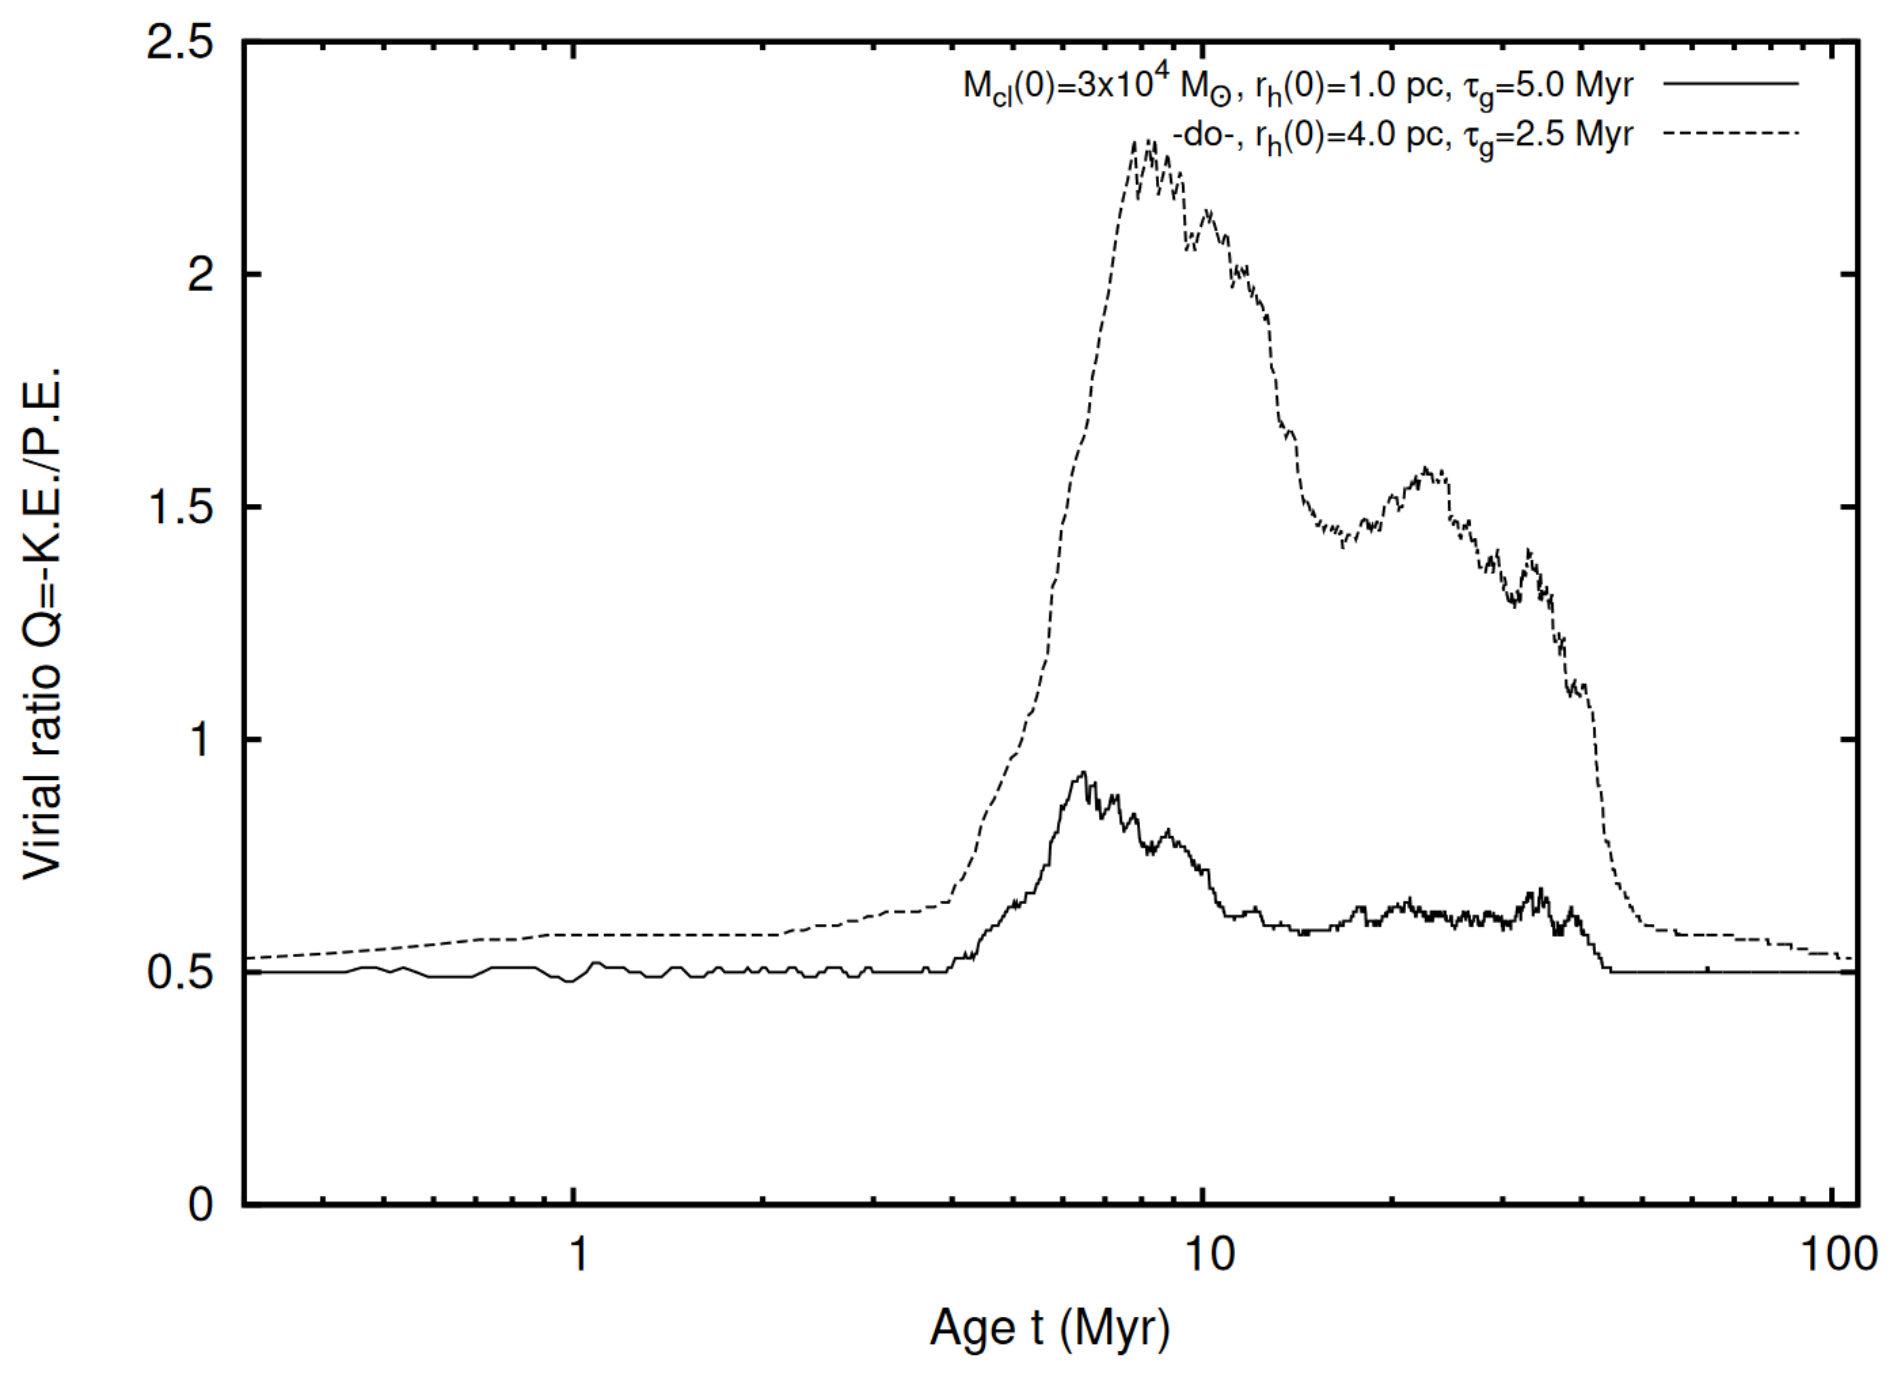
\includegraphics[width=0.8\textwidth]{fig/c1/virialisation_placid_gas_expulsion.png}
	\caption[The evolution of the virial ratio of simulated star clusters with a `placid' model of explosive feedback]{The evolution of the virial ratio of simulated star clusters with a `placid' model of explosive feedback. Simulations were conducted given a cluster of mass  $3\times10^4$~\MSun, with the dashed line showing a cluster with an initial half-mass radius of 1~pc and the solid line showing a cluster with an initial half-mass radius of 4~pc. \emph{Credit}: \cite{banerjee_how_2017}.}
	\label{fig:intro:theory:feedback}
\end{figure}

Once stellar winds expel the initial gas a bound cluster formed from, star clusters in the disk of the Milky Way continue to have a somewhat tumultuous life. Young clusters were typically observed to have sizes larger than those predicted by N-body simulations; it is now believed that other processes must inject energy into early young star clusters in order for them to reach their present-day larger sizes \citep{banerjee_how_2017}.

After initial gas expulsion within the cluster stops additional star formation, star clusters are believed to continue interacting with surrounding gas in their parent GMC for multiple Myr. Stellar winds and feedback from supernovae will continue to disperse the GMC well beyond the radius of the cluster, forming a HII region. This causes a `gravitational feedback' effect, where the massive GMC is blown away and net forces on stars in the cluster also add energy in the system, causing the cluster to be supervirial and undergo a phase of expansion \citep{krause_physics_2020}.

The exact physics of this feedback are still under study, although Fig.~\ref{fig:intro:theory:feedback} taken from \cite{banerjee_how_2017} shows the virial ratio of simulated star clusters with respect to time, for an intermediate or `placid' model of explosive stellar feedback. Within the first 10~Myr of the cluster's lives, feedback causes them to become supervirial. Once the parent GMC has been dispersed, the clusters continue to expand, before eventually reaching dynamical equilibrium and returning to a state with $Q\approx0.5$ after a few tens of Myr. These simulations echo the results of \cite{kuhn_kinematics_2019}, who studied 28 young stellar groups with \gaia\ DR2 and found that 75\% were undergoing expansion (i.e. are supervirial). 

All star clusters are expected to lose a significant portion of their initial mass during this phase of expansion. It has been theorised that bound clusters that form with low initial masses or high initial radii may even be completely destroyed in the initial phase of feedback and expansion, which ought to be visible as unbound cluster remnants \citep{krause_physics_2020}.


\subsubsection{Evaporation and destruction (upto \textasciitilde1~Gyr)}

Since OCs are rarely observed at ages greater than $\sim1$~Gyr, it is clear that some processes eventually destroy them over time. This is believed to happen in three ways.

Firstly, stellar evolution will gradually cause mass loss in a cluster, with more massive stars undergoing supernovae and evolving into compact remnants, losing a significant proportion of their mass in the process. However, since most stars are more compact M, K, or G stars with lifetimes significantly longer than the typical maximum OC lifetime of 1~Gyr, this effect is relatively insignificant during the lifespan of an OC \citep{krause_physics_2020}.

Secondly, clusters gradually lose stars over time in a process known as evaporation. The stars in a cluster will not all have the same velocity; a cluster in dynamical equilibrium will have an isothermal velocity dispersion that is approximately Maxwellian. Some stars with velocities at the tail end of this distribution will have velocities higher than the escape velocity of the cluster $v_\text{esc}$, and will be ejected from the cluster. Over time, two and three-body interactions will accelerate some stars preferentially and ensure that a small proportion of cluster members always have velocities greater than the cluster's $v_\text{esc}$ \citep{portegies_zwart_young_2010,krause_physics_2020}. Stars are preferentially ejected via the cluster's $L_1$ and $L_2$ Lagrange points relative to the tidal field of the Milky Way, which produces the observed tidal tails of many clusters in \gaia\ \citep{portegies_zwart_young_2010,tarricq_structural_2022}. Less commonly, stars will still be ejected in a random direction (opposed to via a Lagrange point), producing an additional spherical `coma' or `corona' of recently ejected stars around a cluster, an effect that has also been observed in \gaia\ data for a number of nearby OCs \citep{meingast_extended_2021,tarricq_structural_2022}.

Finally, star clusters are theorised to be heavily disrupted by tidal `shocks' (perturbations). Reasonably often within every 1~Gyr, star clusters in the Milky Way's disk are expected to come close to or even collide with various pieces of massive galactic structure, such as GMCs or transient spiral arms. The tidal perturbations from these interactions increase the energy of stars in a cluster and should cause considerable mass loss. Due to the rarity of these events, they are yet to be directly observed for OCs in the Milky Way; nevertheless, simple theoretical arguments can show that these events will occur reasonably often for any star cluster in the disk. Especially within the first 1~Gyr of an OC's life, tidal shocks are expected to be a major (and potentially even dominant) method of star cluster destruction.


% ---------------------------------------
\section{The structure of this thesis}
\label{sec:intro:structure}

\textbf{Chapter \ref{sec:intro}} \\[0.2em]
\blindtext

\textbf{Chapter \ref{sec:intro}} \\[0.2em]
\blindtext

\textbf{Chapter \ref{sec:intro}} \\[0.2em]
\blindtext

\textbf{Chapter \ref{sec:intro}} \\[0.2em]
\blindtext

\textbf{Chapter \ref{sec:intro}} \\[0.2em]
\blindtext
   % INCLUDE: introduction

%\part{Additional Example Part}
% !TEX root = ../my-thesis.tex
%
\chapter{Comparison of clustering algorithms applied to \emph{Gaia} DR2 data}
\label{sec:comparison}

\cleanchapterquote{The reward of the young scientist is the emotional thrill of being the first person in the history of the world to see something or understand something. Nothing can compare with that experience.}{Cecilia Payne-Gaposchkin}{(1977)}

\authorship{The content of this chapter is almost entirely based on work published in \cite{hunt_improving_2021}. I conducted all scientific work and wrote all of the text. Suggestions and corrections from my supervisor and the reviewer of the paper are included in the text. The formatting of figures and tables has been adjusted to better fit the formatting of this thesis.}



\section{Introduction}

Open clusters (OCs) are commonly known as the laboratories of stellar evolution, which form when large gas clouds collapse into dense, gravitationally bound regions of stars. The stars in OCs have roughly the same age and chemical composition, meaning that every OC is a unique `experiment' showing the results of stellar evolution with stars across a range of masses given a certain set of initial conditions. In particular, OCs in our own galaxy are the most enlightening to study, since their proximity means that individual stars can be resolved and parameters can be determined to higher levels of precision.

The number of known open clusters has not changed significantly until recently. The New General Catalogue (NGC) listed $\approx$700 objects that we now know to be OCs \citep{dreyer_new_general_1888a}, the most comprehensive catalogue of its time -- yet over a century later, the catalogue of \cite{mermilliod_database_1995} had only increased to a size of ~1200 OCs, not even doubling the OC census despite the large strides in astronomical instrumentation and data analysis taken in the 20th century. In part, this is because numerous clusters in the literature were ruled out as associations by modern data, reducing the size of the census -- yet it still persists that a century of work did not significantly increase the size of the OC census.

The largest increases to the size of the census came with the advent of new techniques. The space-based astrometric survey of the \emph{Hipparcos} satellite \citep{hog_tycho-2_2000} revealed a number of new, often relatively sparse OCs in studies such as \cite{platais_search_1998} and \cite{chereul_distribution_1999}, while wide-field infrared surveys looked through interstellar extinction to find new OCs in studies such as \cite{dutra_new_2001} and \cite{froebrich_systematic_2007}. The catalogue of \cite{kharchenko_global_2013} (hereafter MWSC) lists 2267 probable OCs and a further 132 that showed nebulosity, a major increase from the figure of \cite{mermilliod_database_1995} just two decades prior.

The next major increase to the size of the OC catalogue is currently in progress thanks to the \emph{Gaia} satellite \citep{brown_gaia_2018}. \emph{Gaia} maps the stars of the Milky Way in five dimensions (positions, proper motions, and parallax), while also providing visual photometry and colours in its own $G$, $G_{BP}$, and $G_{RP}$ photometric bands, and spectroscopic radial velocities for a small sample of bright stars. Compared with \emph{Hipparcos}, \emph{Gaia} has roughly an order of magnitude more precision in astrometric parameters for $10^4$ times as many stars, resulting in a groundbreaking dataset that has full astrometric solutions and photometry for 1.3 billion stars as of \emph{Gaia} DR2, 7 million of which also have radial velocities.

It is perhaps unsurprising that such a large improvement in our ability to map the galaxy is also greatly improving the OC census. In terms of quantity, works such as \cite{castro-ginard_new_2018,castro-ginard_hunting_2019,castro-ginard_hunting_2020}, \cite{liu_catalog_2019}, \cite{sim_207_2019}, and \cite{cantat-gaudin_gaia_2019} have recently reported hundreds of candidate OCs using \emph{\review{Gaia}} data. Typically, this is done using automated blind searches of the \emph{\review{Gaia}} dataset with clustering algorithms -- a type of unsupervised machine learning that can find the most natural groupings or clusters within a dataset, requiring only basic parameters and minimal prior knowledge about the structure of the data.

The precision of \emph{Gaia} is also improving the quality of the OC census. While traditionally, distances to OCs would be derived using photometry alone and fitting a model-dependent stellar isochrone to the OC's colour-magnitude diagram, \emph{Gaia} parallaxes provide an unbiased and model-independent distance estimator -- allowing parameters for OCs to be derived to greater levels of precision \review{\citep[e.g.][]{cantat-gaudin_painting_2020}
}. \cite{cantat-gaudin_gaia_2018} derive membership lists and parameters for 1229 OCs using \emph{Gaia} DR2 data alone, which has been expanded with some re-analysis and by including recently detected clusters in \cite{cantat-gaudin_clusters_2020}. It is expected that some OCs listed in MWSC will not be detectable in \emph{Gaia} data. \emph{Gaia}'s visual band observations are unable to see into areas of high dust extinction unlike the infrared photometry used by MWSC -- obscuring small, distant OCs from view in regions with high extinction, such as towards the galactic centre at distances greater than $\sim3$ kpc. In addition, parallaxes and proper motions have fractional uncertainties that increase with distance, which has a significant negative effect on the signal to noise ratio of OCs in \emph{Gaia} data at distances larger than $\sim1-3$ kpc.

However, despite astrometric uncertainties or dust obscuring \emph{Gaia}'s view of some clusters, it is also possible to rule out a number of OCs that should still be detectable in \emph{Gaia} data based on their existing parameters. \cite{cantat-gaudin_clusters_2020} have ruled out 38 OCs in the literature as asterisms, all of which should be bright enough to detect in the \emph{Gaia} dataset based on their reported parameters but do not appear to exist. Future studies will be able to rule out yet more putative OCs based on \emph{Gaia} data alone, particularly as \emph{Gaia} data improves in the coming years with future releases.

In its current state, the OC census is difficult for astronomers to use. Despite MWSC deriving that the OC census was complete to within 1.8 kpc, the recent myriad of studies using \emph{Gaia} data have shown that many more OCs are yet to be discovered within the immediate solar neighbourhood. Until the OC census is shown to be complete to within a certain radius, it is impossible to calculate accurate population statistics about OCs in the Milky Way. In addition, the many asterisms that are not yet concretely ruled out in the literature make the OC census more difficult to use, as not all reported OCs in the literature are really there and many do not make good targets for precious telescope time.

Within the next decade, future data releases of the \emph{Gaia} satellite and large-scale spectroscopic surveys such as 4MOST \citep{de_jong_4most_2012} will provide astronomers with a wealth of data on on our galaxy. OCs are an important piece of the jigsaw puzzle of the Milky Way's current and past star formation. An OC census with greatly improved quality and quantity will allow astronomers to use the census reliably for a \review{range }of scientific purposes, including mapping the age distribution of OCs across the galaxy \citep{cantat-gaudin_painting_2020, yen_reanalysis_2018}, studies of the chemical composition of OCs \citep{baratella_gaia-eso_2020, donor_open_2020}, to even studying the conditions of planet formation in OCs and the implications that may have for the distribution of the wider exoplanet census \citep{fujii_survival_2019}.

To date, a number of different methods have been used to search for new or existing OCs in \emph{Gaia} data. While UPMASK \citep[Unsupervised Photometric Membership Assignment in Stellar Clusters,][]{krone-martins_upmask:_2014} as used by \cite{cantat-gaudin_gaia_2018} and \cite{cantat-gaudin_clusters_2020} is a highly successful tool for producing membership lists of existing OCs, it is too slow to conduct a large-scale blind search across the billion star dataset of \emph{Gaia}. In turn, while approaches such as the one applied in \cite{castro-ginard_hunting_2020} has detected hundreds of new OCs in the \emph{Gaia} dataset, their method is unable to detect a large fraction of literature OCs, suggesting that their approach may also be unable to detect a large fraction of as yet undiscovered OCs with similar properties. Different approaches have advantages and disadvantages that have never before been compared side-by-side on \emph{Gaia} data, and no single approach has yet been developed that can simultaneously detect new OCs in a large-scale blind search while also detecting a majority of already-reported objects.

In this series of papers, we will work to improve the OC census: primarily by attempting to detect new OCs, but also by re-detecting a large fraction of literature OCs with a different methodology and complementing cataloguing efforts such as \cite{cantat-gaudin_clusters_2020}. In this study, we create an unbiased preprocessing pipeline to prepare \emph{Gaia} data for analysis by clustering algorithms, and test the ability of three clustering algorithms to detect OCs in \emph{Gaia} data. In Sect.~\ref{c2:sec:data}, we describe the \emph{Gaia} data used and the applied pre-processing steps. Section~\ref{c2:sec:algorithms} outlines the requirements for any clustering algorithm to be applied to \emph{Gaia} data and describes three chosen algorithms that meet these criteria. Our analysis process for the algorithms applied to our data and the results of this are presented in Sect.~\ref{c2:sec:results}. In Sect.~\ref{c2:sec:discussion}, we discuss the strengths and weaknesses of each approach and the implications for future studies. \review{We report on 41 new OC candidates discovered during the preparation of this paper in Sect.~\ref{c2:sec:new_ocs}. Finally, Sect.~}\ref{c2:sec:conclusion} summarises our results.


%--------------------------------------------------------------------


\section{Data}\label{c2:sec:data}
\subsection{The \emph{Gaia} DR2 dataset and the HEALPix system}

\begin{figure*}
   \centering
   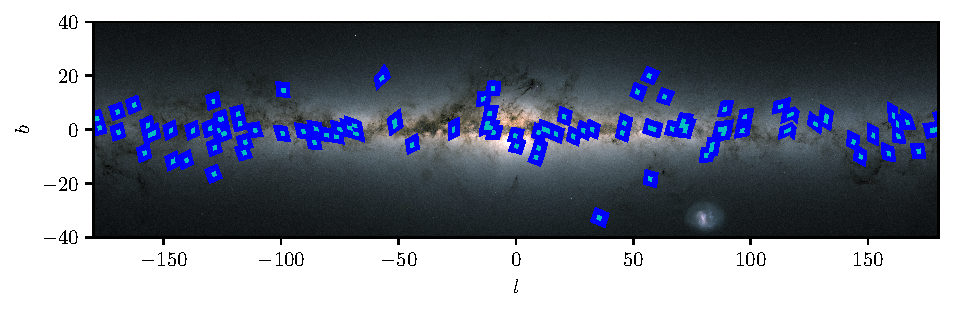
\includegraphics[width=\textwidth]{fig/c2/fig_fields.pdf}
   \caption[Target fields for this study plotted above a  \emph{\review{Gaia}} map of stellar density in an equirectangular projection]{Target fields for this study plotted above a  \emph{\review{Gaia}} map of stellar density in an equirectangular projection. Cyan regions show the 100 main HEALPix level five pixels. Each main pixel was merged with its eight nearest neighbours, which are shown in blue. Some nearest neighbour pixels overlap between different fields.}\label{c2:fig:targetfields}%
\end{figure*}

The results of any unsupervised search for OCs are always highly dependent on the input data and how it is preprocessed: assumptions must be made for reasons of computational efficiency (for instance, splitting the dataset into separate chunks to improve runtime), and dimensions of the data with different units and coordinate systems must be intelligently preprocessed to allow an unsupervised algorithm to take full advantage of \emph{Gaia} data. We briefly introduce the \emph{Gaia} satellite and explain the preprocessing pipeline we developed to prepare its data for use with unsupervised clustering algorithms.

The \emph{Gaia} satellite is producing a previously unprecedented quantity and quality of astrometric and photometric data for stars in the Milky Way. 1.7 billion sources brighter than $G=21$ are included in \emph{Gaia} DR2, where 1.3 billion have full five-parameter astrometric solutions. Uncertainties on derived parameters for each source depend strongly on the brightness of the source. While as many detected sources as possible are included in \emph{Gaia} DR2 for completeness, the majority of faint sources are not useful for studies of galactic structure as the uncertainties on their parameters are too large. 

For example, a star with brightness $G=17$ would have corresponding uncertainties of 0.1 mas in parallax and 0.2 mas yr$^{-1}$ in proper motion \citep{brown_gaia_2018}. If this star is 1 kpc away and hence has a true parallax of 1 mas, a measured parallax for this star would be informative to within roughly 10\% of the true distance. The uncertainty on proper motion for this star would easily allow it to be distinguished as a member of an open cluster, as open clusters at this distance typically have an inherent proper motion dispersion of $\sim$1 mas yr$^{-1}$ which is larger than the star's proper motion uncertainty. However, a faint star with $G=20$ at a true distance of 1 kpc will have corresponding uncertainties of 0.7 mas in parallax and 1.2 mas yr$^{-1}$ in proper motion. Any parallax measurement for this star will be much less informative about the star's true distance, with a near 100\% fractional uncertainty. Its proper motion uncertainty is larger than the typical dispersion of proper motion in OCs at 1 kpc, meaning that this faint star could never be reliably assigned as a member of an OC with \emph{Gaia} DR2.

As such, most studies adopt a cut on the dataset to ignore uninformative stars and improve the signal to noise ratio of open clusters in the \emph{Gaia} data. For the purposes of this study, we cut all stars fainter than $G=18$, corresponding to typical maximum uncertainties of 0.15 mas in parallax and 0.3 mas $yr^{-1}$ in proper motion, which is the same magnitude cut as used by \cite{cantat-gaudin_gaia_2018} and \cite{liu_catalog_2019}, although \cite{castro-ginard_hunting_2020} adopt a stronger cut at $G=17$.

Some studies \citep[such as][]{castro-ginard_hunting_2020, liu_catalog_2019} also remove outlier stars based on the magnitude of their proper motions or parallaxes. We choose not to remove stars with negative parallaxes, as this would make our study less sensitive to the most distant clusters for which member stars may have zero or negative parallax values. We also do not remove stars with high proper motions -- while very few open clusters have proper motions $\mu_{\alpha*}$ or $\mu_\delta$ of greater than 30 mas yr$^{-1}$, we still wish to have as few biases as possible in this study.

To select regions of the sky for study, we use the HEALPix\footnote{\href{http://healpix.sourceforge.net}{http://healpix.sourceforge.net}} (Hierarchical Equal Area isoLatitude Pixelization) scheme \citep{gorski_healpix:_2005} to select equal-area approximately quadrilateral regions of the \emph{\review{Gaia}} dataset. HEALPix has advantages over rectangular tesselation schemes \citep[such as those used in][]{castro-ginard_hunting_2020} since spherical distortions from projecting quadrilaterals onto the sky are spread out, allowing algorithms to be ran on equal-area pixels. In addition, \emph{Gaia} sources are numbered based on a HEALPix system, making the HEALPix system convenient for a study of \emph{Gaia} data to implement.

We aim to tile the sky into manageable chunks: large enough to contain OCs beyond a certain distance, but not so large that the amount of data in each chunk becomes prohibitively computationally expensive to run on. These chunks should also be easy to overlap, so that our future blind searches would not have edge effects. To do this, we select a region of study and its HEALPix level five pixel. The eight nearest pixels to each central pixel are added to each region of data to analyse, creating chunks each of area $\sim 31$ deg$^2$ and side length approximately 5$^\circ$. 0.2\% of HEALPix pixels only have seven neighbours and will hence have slightly smaller areas. It may be difficult to detect OCs closer than $\sim$350 pc with this tiling scheme since a typical OC at this distance may have a larger tidal radius that the data field. Any future blind search would be supplemented with a clustering analysis in Cartesian co-ordinates of all stars within 500 pc, solving this issue and also allowing nearby OCs to be properly detected without issues stemming from spherical distortions at angular separations greater than roughly $\sim10^{\circ}$.

HEALPix is straightforward to use with \emph{Gaia} data, since all stars are numbered based on the HEALPix pixels they are present in. For a given \texttt{source\_id}, its HEALPix pixel at level $n$ is given by:

\begin{equation}\label{c2:eqn:healpix}
    \textrm{HEALPix pixel} = \textrm{FLOOR} \left( \frac{\texttt{source\_id}}{2^{35} \cdot 4^{12-n}}  \right).
\end{equation}

\noindent
For efficiency when querying the \emph{Gaia} database with ADQL, this formula is inverted and used to select all stars with a \texttt{source\_id} in the correct range of values. When downloading the stars in a given pixel, we require that all sources have a full five-parameter astrometric solution, valid $G_{BP}$ and $G_{RP}$ photometry, and a $G$-band magnitude less than 18. An exact copy of the ADQL query used for this study is included in Appendix~\ref{app:c2:adql}.

%--------------------------------------------------------------------
\subsection{Selection of target fields}

To study the effectiveness of clustering algorithms across a representative sample of stellar densities, we randomly selected 100 objects from MWSC that were each in unique HEALPix level five pixels. This list of 100 objects formed a list of 100 `main objects' to study. The eight nearest pixels to each central pixel were added to each of the 100 selected pixels to analyse. This resulted in 100 separate chunks, with 733 unique HEALPix level five pixels out of 900 in total since the neighbour pixels of different chunks were allowed to overlap. The fields are shown in Fig.~\ref{c2:fig:targetfields} and listed in Appendix~\ref{app:c2:fields}. \review{The fields contained between 100$\,$000 to 4.2 million stars, with a mean of 734$\,$000 stars. In total, all fields contain 56.8 million unique stars, representing $\approx$20\% of the 260 million stars in }\emph{\review{Gaia}} \review{DR2 brighter than $G=18$.
}

All but one of these fields are in the galactic disk with $|\,b\,|<25^{\circ}$, and many of them are situated in areas of dense star formation where many OCs are present. We accidentally selected two globular clusters in our main list that did not contain any OCs centrally located in their field, which we replaced in our main list of 100 OCs with OCs from fields 14 and 57. To expand the target list from the initial 100 OCs to include other OCs contained within these fields, we searched the catalogues of MWSC, \cite{cantat-gaudin_clusters_2020}, \cite{castro-ginard_hunting_2020} and \cite{liu_catalog_2019}, which contain \review{a total sum of 4002 reported OCs}. We required that reported OCs in the literature be entirely contained by a field given their reported radius and distance \review{to mitigate edge effects which could cause non-detections}. For \cite{cantat-gaudin_clusters_2020} OCs, $2 \cdot r_{50}$ (the radius containing half of the members of the OC) was used as a proxy for tidal radius. For the catalogue of \cite{castro-ginard_hunting_2020}, which \review{lists Gaussian angular dispersions $\theta$ containing $\sim68$\% of members, $2 \cdot \theta$ was used as a proxy for tidal radius}. In total, the literature reports \review{1385 }unique OCs contained within the 100 fields, all of which should be entirely visible and not partially clipped by the fields' edges. This represents roughly a third of the total number of clusters that the above four works report.

\review{The objects in MWSC that remain undetected in }\emph{\review{Gaia}} \review{data present a particular challenge for the algorithms in this study. }Since \cite{cantat-gaudin_clusters_2020} have found that a number of clusters listed in MWSC are not real, we do not expect any algorithm to detect OC candidates corresponding to all listed targets\review{, meaning that most MWSC targets are false positives that should be discarded by the algorithms. However, a small number of MWSC objects may be real but are simply as yet undetected in }\emph{\review{Gaia}} \review{data due to limitations of the methodologies used. Hence, the inclusion of MWSC objects allows us to test the ability of the algorithms to rule out putative objects, corresponding to their true and false negative rates, while also testing the algorithms against the sensitivity of existing approaches and seeing if any additional MWSC targets can be recovered in \emph{Gaia} data with new methodologies. }We chose to use real \emph{Gaia} data for our study instead of simulated data so that we can develop our full pipeline from start to finish to work with real data, which includes a number of challenging aspects \cite[such as systematic errors on astrometric parameters,][]{lindegren_gaia_2018} that would not be adequately tested by using simulated data only.


%--------------------------------------------------------------------
\subsection{Preprocessing steps}

In the limit of small errors, clustering analysis could be performed with three-dimensional spatial data in a Cartesian frame. However, parallaxes are inherently difficult to measure and have large fractional uncertainties in \emph{Gaia}, and transforming the spherical co-ordinate system of \emph{Gaia} data to Cartesian co-ordinates is non-trivial and would introduce large errors to other axes of the data. As such, it is easier to remain in a spherical co-ordinate system to avoid contaminating positional data with the large errors of parallax measurements. Searches for OCs are helped immensely by proper motions, as OCs are gravitationally bound groups of stars that appear tightly clumped in proper motion space. These could be changed to Cartesian velocities with parallaxes, but this is avoided for the same reasons as with positions. 

Attempts were made to use distances instead of parallaxes with the distance catalogue of \cite{bailer-jones_estimating_2018}. However, while their method is appropriate for macroscopic studies of galactic structure, it places stars with uncertain parallaxes at a prior-defined distance, which moves low magnitude member stars further from their parent OCs in the data and was found to reduce the signal to noise ratio of OCs in the data. \review{Alternative distance estimators that are better at preserving small scale galactic structure could be investigated in the future, }such as StarHorse \citep{anders_photo-astrometric_2019} \review{which uses }magnitude information and stellar models to increase the accuracy of \emph{Gaia}-derived distances.

Some pre-processing can be done to reduce the effect of remaining in a spherical co-ordinate system and using parallaxes instead of distances, but without contaminating other dimensions of the data with the large uncertainties of parallax measurements. To remove spherical distortions that occur at high latitudes in position and proper motions, every field is rotated to an arbitrary co-ordinate frame $(\lambda, \, \phi)$ centred at (0,0) and rotated to have edges parallel with the co-ordinate axes for neater plotting of individual fields, with proper motions $\mu_{\alpha*}$, $\mu_{\delta}$ also transformed to the new frame as $\mu_{\lambda*}$, $\mu_{\phi}$. 

Machine learning algorithms benefit from having scaled inputs, so the five dimensions of data for each field $(\lambda, \, \phi, \, \mu_{\lambda*}, \, \mu_{\phi}, \, \varpi)$ are re-scaled to have a median of zero and a unit inter-quartile range using a \texttt{RobustScaler} object from \texttt{scikit-learn} \citep{pedregosa_scikit-learn_2011}. This process is resilient to outliers, unlike scaling to have zero mean and unit variance as is sometimes used in the literature. This re-scaling process also ensures that each co-ordinate axis has an equal weight when passed to clustering algorithms. We choose not to experiment with re-weighting dimensions of the dataset as was performed tentatively by \cite{liu_catalog_2019}, although this could be explored in future works.


%--------------------------------------------------------------------

\section{Selection and implementation of clustering algorithms}\label{c2:sec:algorithms}
\subsection{Criteria}\label{c2:sec:algorithms_criteria}

% Algorithms table
\begin{table}
\caption[Algorithms considered for inclusion by this study]{Algorithms considered for inclusion by this study.}
\centering
\begin{tabular}{l c c c}
\hline\hline
          & Runtime & Deals with & Open-  \\
Algorithm & scaling\tablefootmark{a} & noise      & source \\
\hline                        
KMeans                & $n$        & No  & \texttt{sklearn}\tablefootmark{b} \\
Affinity propagation  & $n^2$      & No  & \texttt{sklearn}\tablefootmark{b} \\
Mean-shift            & $n^2$      & No  & \texttt{sklearn}\tablefootmark{b} \\
Spectral              & $n^3$      & No  & \texttt{sklearn}\tablefootmark{b} \\
Ward                  & $n^3$      & No  & \texttt{sklearn}\tablefootmark{b} \\
Agglomerative         & $n^3$      & No  & \texttt{sklearn}\tablefootmark{b} \\
DBSCAN                & $n \log n$ & Yes & \texttt{sklearn}\tablefootmark{b} \\
OPTICS                & $n^2$      & Yes & \texttt{sklearn}\tablefootmark{b} \\
Gaussian mixtures     & $n$        & No  & \texttt{sklearn}\tablefootmark{b} \\
Birch                 & $n$        & No  & \texttt{sklearn}\tablefootmark{b} \\
Friend of Friends     & $n \log n$ & No  & \texttt{pyfof}\tablefootmark{c} \\
HDBSCAN               & $n \log n$ & Yes & \texttt{HDBSCAN}\tablefootmark{d} \\
\hline

\end{tabular}

\tablefoot{
\tablefoottext{a}{Runtime scalings are best case estimates and are only given with respect to number of data points $n$.}
\tablefoottext{b}{\href{https://scikit-learn.org/}{https://scikit-learn.org/}}
\tablefoottext{c}{\href{https://pypi.org/project/pyfof/}{https://pypi.org/project/pyfof/}}
\tablefoottext{d}{\href{https://pypi.org/project/hdbscan/}{https://pypi.org/project/hdbscan/}}
\label{c2:tab:algorithms}
}

\end{table}

While many clustering algorithms exist in the literature, the complexities of \emph{Gaia} data make only a few appropriate for a large-scale unsupervised OC search. In future works, we will run on the $\approx 200$ million stars in \emph{Gaia} data brighter than $\text{G}=18$, only a small fraction of which reside in OCs. Individual fields can contain up to approximately five million stars. Hence, any clustering algorithm would need to be extremely efficient at searching through a large quantity of data to find rare objects that require a high degree of sensitivity to detect.

In later parts of this work, we compare the performance of the clustering algorithms we selected. However, to be selected for further study, the algorithms must be even remotely practical for use with \emph{Gaia} data. We set the following basic requirements on clustering algorithms for inclusion in this study. Firstly, it must be fast enough to run on the entire \emph{Gaia} dataset with a few weeks of wall time on a relatively powerful computer. Secondly, it must be able to deal with unclustered field stars (noise), as only a small fraction of stars in the Milky Way reside in OCs and the rest must be discarded. Finally, an open-source implementation must be readily available in the literature for the algorithm.

The performance of all clustering algorithms against these criteria listed in the \texttt{scikit-learn} \citep{pedregosa_scikit-learn_2011} Python library, in addition to two other common algorithms considered here, is listed in Table~\ref{c2:tab:algorithms}. The galaxy cluster detection algorithm AMICO \citep[Adaptive Matched Identifier of Clustered Objects,][]{bellagamba_amico:_2018} was also investigated for this work, but necessary modifications to the algorithm were not made in time to adapt it for use with \emph{Gaia} data. AMICO was a top performing algorithm on mock \emph{Euclid} data \citep{euclid_collaboration_euclid_2019}, and so its application to OC detection would still be worth investigating in the future.

The first criterion disqualifies the vast majority of clustering algorithms in the literature. Practically, algorithms with runtime complexities of $\mathcal{O} ( n^2 )$ or worse (where $n$ is the number of stars) are too slow to run on large segments of the \emph{Gaia} dataset. For instance, while OPTICS \citep{ankerst_optics_1999} has seen some use in astronomy analysing smaller portions of the \emph{Gaia} dataset -- such as by \cite{ward_not_2019}, who used OPTICS to detect OB associations -- its $\mathcal{O} ( n^2 )$ runtime complexity was found to be prohibitively slow for inclusion in this work.

The second criterion favours density-based clustering algorithms such as DBSCAN \citep[Density-Based Spatial Clustering of Applications with Noise,][]{ester_density-based_1996} and HDBSCAN \citep[Hierarchical DBSCAN,][]{hutchison_hdbscan_2013}, which are the  only class of clustering algorithm that can discard points that are not in locally dense regions. These algorithms use nearest-neighbour distances to infer the local density around points, with points in low density regions discarded as field stars. However, some success has also been had in the literature with using fast algorithms to partition all data and only keep partitions that look like OCs, such as with Gaussian mixture models \citep[hereafter GMMs]{dempster_maximum_1977} by \cite{cantat-gaudin_gaia_2019}. A simple cut on proper motion dispersion can be enough to discard most non-OC partitions. The third criterion is unrestrictive, as open-source implementations exist for all algorithms that will be considered in this study.

Three algorithms were selected for further study. Firstly, DBSCAN, as mentioned previously, is a fast density-based clustering algorithm with excellent scalability, that has already proven itself in the literature in the blind searches of \cite{castro-ginard_new_2018, castro-ginard_hunting_2019, castro-ginard_hunting_2020}, recently finding hundreds of new OCs in \emph{Gaia} data. 

The second algorithm, HDBSCAN, is also density-based but improves upon DBSCAN by clustering the data hierarchically, allowing it to deal with areas of different densities better and theoretically giving it greater sensitivity. Its parameters are different to DBSCAN, and may or may not be easier to tune. It has been used by \cite{kounkel_untangling_2019} and \cite{kounkel_untangling_2020} to probe the \emph{\review{Gaia}} dataset for spatially correlated moving groups within 3 kpc, but has never been used purely to search for OCs and across all distance scales in the \emph{Gaia} dataset.

Finally, GMMs were selected for trial, an algorithm unlike DBSCAN or HDBSCAN in that it must partition all data, and partitions not containing OCs must be discarded. In principle, this could be a fast method, as GMMs have $\mathcal{O} ( n )$ runtime. A method similar to that of \cite{cantat-gaudin_gaia_2019} should be used to discard unclustered field stars with this algorithm. In addition, since it fits a model directly to the data instead of using nearest-neighbour distances, it should be less sensitive to the preprocessing or underlying shape of the data.

Some algorithms were not included in this study as their performance is clearly superseded by one of the three above. K-Means \citep{macqueen_methods_1967} is a partitioning algorithm similar to GMMs that fits a user-specified number of centroids to a dataset. Points are assigned to their nearest centroid. However, this algorithm was found to perform poorly on the \emph{Gaia} dataset, as the five dimensions of the data have intrinsically different scales. A distant cluster will have a near-negligible size in positional space, but will still form a Gaussian clump in proper motion and parallax spaces due to the dominance of \emph{\review{Gaia}} errors at these distances. Alternatively, a nearby cluster will have large sizes in position and proper motion spaces, but still a relatively small parallax dispersion as all stars are at roughly the same distance. K-Means will routinely over or under-select cluster stars without extremely careful pre-processing, as it cannot re-scale its model independently for each axis of the data. However, GMMs can, since they fit a multivariate Gaussian. As such, including K-Means in this study was unnecessary, as GMMs are effectively a generalisation of the K-Means algorithm that allows each cluster to have a covariance matrix (i.e. a different scale for each axis.) In a similar vein, while Birch \citep{zhang_birch_1996} is similar to K-Means clustering but makes a number of improvements, it also struggles to deal with clusters that have different scales in each dimension for the same reasons.

The Friend of Friends (FoF) algorithm has also been used in the literature \citep{liu_catalog_2019} and has a history of use in astronomy, especially in searches for dwarf galaxies \citep[e.g.][]{duarte_how_2014} or dark matter haloes. However, it was not included in this study as it is the same as running DBSCAN with the minimum number of points ($m_{Pts}$) parameter set to 1, since both algorithms use a global density parameter and a notion of core or border points -- or `friends' and `friends of friends' in the FoF algorithm. However, the addition of $m_{Pts}$ to DBSCAN allows it to deal with unclustered points by discarding small clusters, which is a clear advantage for \emph{Gaia} data and in line with our second criterion -- whereas users of the FoF algorithm must manually discard small clusters.

In the following sub-sections, each selected algorithm will be explained in brief detail, along with any steps necessary to determine their parameters.


%--------------------------------------------------------------------
\subsection{DBSCAN}

\begin{figure}[t]
   \centering
   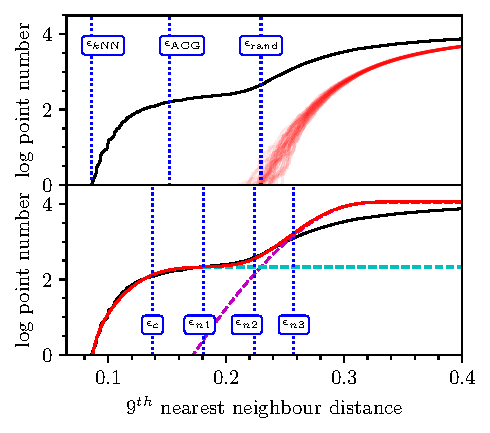
\includegraphics[width=0.7\textwidth]{fig/c2/fig_dbscan.pdf}
   \caption[Nearest neighbour graphs for both methods of determining the optimum $\epsilon$ for DBSCAN]{Nearest neighbour graphs for both methods of determining the optimum $\epsilon$ for DBSCAN. To produce this plot, which is effectively an unnormalised log cumulative density function (CDF) of nearest neighbour distances, stars are sorted based on their $k^{\text{th}}$NN distances and numbered from one to $n$. These labels as a function of $k^{\text{th}}$NN distance are then plotted to form a continuous curve. The black line on both plots is the $9^{\text{th}}$NN distances of a 2.5$^\circ$ field around the nearby OC Blanco 1. On the upper plot, $\epsilon$ estimates are determined by re-sampling the field 30 times (shown in red) to smooth out the signature of clustered stars. On the lower plot, a model of the signature of the cluster (cyan, dashed) and the field (magenta, dashed) is summed (red, solid) to approximate the curve and produce four $\epsilon$ estimates.}\label{c2:fig:dbscan}%
\end{figure}

\subsubsection{Description of algorithm}

DBSCAN \citep{ester_density-based_1996} is one of the oldest and most widely used density-based clustering algorithms in the literature. It works by using the distances between points as a proxy for the local density of an area in a dataset, with the densest areas labelled as clusters and sparse regions labelled as unclustered background noise. Clusters are selected using two parameters. Firstly, points in a dataset are labelled as $\epsilon$-reachable if the distance between them is lower than some threshold $\epsilon$. Secondly, points are labelled as core points if they are $\epsilon$-reachable to at least $m_{Pts}$ other points, or border points if they are not core points but are $\epsilon$-reachable to a core point, where $m_{Pts}$ also includes the considered point itself. Finally, clusters are selected as density-connected groups of points that are $\epsilon$-reachable via a core point, with all other points labelled as noise.

In this way, it follows that setting $\epsilon$ to a very large value would cause all points to be labelled as one cluster, and setting $\epsilon$ to a very small value would cause no points to be labelled as cluster members. The key is to set $\epsilon$ to an appropriate value, such that separate clusters are not accidentally merged by the algorithm, and such that the algorithm is still sensitive to sparse clusters that are only marginally denser than surrounding noise points. However, this is difficult for datasets of variable density, since $\epsilon$ is a global parameter. This is a particular issue for \emph{Gaia} data, since the density of the dataset is highly variable: due to the spherical projection of \emph{Gaia} data, the density of the dataset changes with distance, since higher distances sample a larger angular volume. In addition, fields that include opaque clouds have variable densities on scales of less than 1$^\circ$, since the high levels of extinction in the clouds reduces the completeness of the \emph{Gaia} instrument. Hence, a key challenge with using DBSCAN on \emph{Gaia} data is choosing values of $\epsilon$ that are a good enough fit to the entirety of every field under study.

The $m_{Pts}$ parameter must be set high enough to restrict the core point label to only the most densely connected points, but not so high that even real clusters do not contain enough points to generate core points. In practice, $m_{Pts}$ and $\epsilon$ do not act independently, with a different choice of $\epsilon$ able to largely reproduce the same result for most values of $m_{Pts}$. As such, $m_{Pts}$ can be set to the most efficient choice. \cite{ester_density-based_1996} suggest setting $m_{Pts}$ to twice the number of dimensions of the dataset, as higher values are more computationally intensive but do not appear to include more information. For the 5D \emph{Gaia} dataset, this would imply setting $m_{Pts}=10$, which also sets a threshold on the minimum size of an OC candidate at ten stars.

By far the most computationally expensive part of the algorithm is the computation of nearest neighbour distances. This is greatly sped up by using a $k$-d tree to calculate nearest neighbour distances efficiently, which is used by the \texttt{scikit-learn} \citep{pedregosa_scikit-learn_2011} implementation of DBSCAN which is used in this work.

In the following subsections, two methods for determining $\epsilon$ for each field are presented, which are both be compared by this study.


\subsubsection{Parameter determination with the Castro-Ginard et al. (ACG) method}

\cite{castro-ginard_new_2018} have developed a method for determining $\epsilon$ for \emph{Gaia} data that exploits the random, unclustered nature of field stars to produce consistent $\epsilon$ estimates (hereafter abbreviated as the ACG method.) A brief description of how it works follows. 

Firstly, a $k^{th}$ nearest neighbour graph is computed for the dataset, where $k = m_{Pts} - 1$ (since $m_{Pts}$ includes each point itself whereas $k$ is the distance to the nearest neighbouring point.) The smallest $k^{th}$ nearest neighbour distance $\epsilon_{k\text{NN}}$ is recorded. 

Secondly, the data are randomly re-sampled according to the overall distribution of astrometric parameters in a given field. Assuming that the contribution of a cluster to this distribution is small as very few stars reside in OCs, the signature of the cluster is removed in the randomly redrawn nearest neighbour graph, allowing it to approximate the distribution of field stars in the dataset. Its minimum $k^{th}$ nearest neighbour distance $\epsilon_{\text{rand}}$ is recorded. This step can be repeated multiple times to take a more accurate mean value of $\epsilon_{\text{rand}}$. \cite{castro-ginard_new_2018} repeat this step 30 times.

Finally, the average of these two values $\epsilon_{\text{ACG}} = (\epsilon_{k\text{NN}} + \epsilon_{\text{rand}}) \, / \, 2$ is used as $\epsilon$ by DBSCAN. When a cluster is present in a field, $\epsilon_{\text{ACG}}$ roughly approximates the modal $k^{th}$ nearest neighbour value for the cluster. When no cluster is present in a field, $\epsilon_{\text{ACG}} \approx \epsilon_{k\text{NN}} \approx \epsilon_{\text{rand}}$, and no clusters will be erroneously detected by DBSCAN.

The ACG method is explained in more depth in \cite{castro-ginard_new_2018}. The top panel of Fig.~\ref{c2:fig:dbscan} shows how random re-sampling allows $\epsilon_{\text{ACG}}$ to be calculated. The implementation of this method differs slightly from the original used by \cite{castro-ginard_new_2018}, as random re-draws in the second step are performed by randomly re-using existing parameter values for stars instead of first averaging them with kernel density estimation, as this was found to produce equivalent results while being somewhat faster.

In \cite{castro-ginard_new_2018, castro-ginard_hunting_2020}, the size of the field under study and the parameter $m_{Pts}$ are also varied across a number of different values, helping to reduce the effect of DBSCAN's global density parameter and detect OCs of different densities. Instead, we trialed varying only $\epsilon$ with the following method, as we expect this will produce similar results while being more computationally efficient: changing the size of the field requires re-calculating the array of nearest neighbour distances, whereas only varying $\epsilon$ means that the array can be cached and efficiently re-used for new parameter values. In practice, one could also vary $\epsilon$ with the ACG method by using different multiples of $\epsilon_{\text{ACG}}$ (e.g. $1.5 \cdot \epsilon_{\text{ACG}}$ or $2 \cdot \epsilon_{\text{ACG}}$).


\subsubsection{Parameter determination with a model-fitting method}

While consistent, the ACG method is slow. Since $k^{th}$ nearest neighbour determination is the most computationally expensive part of DBSCAN, repeating it 30 times to randomly estimate $\epsilon_{\text{rand}}$ increases the runtime of DBSCAN by a factor of about 30. Instead, a model-fitting method was devised in this study to perform fast approximate analyses of the $k^{th}$ nearest neighbour graph of a field.

Instead of numerically differentiating this graph to find turning points and hence an optimum value for $\epsilon$, fitting a simple, approximate model is significantly more consistent and numerically stable. A cluster can be made up of just a few dozen stars projected against tens of thousands of background stars, complicating numerical differentiation since the signal of a cluster in such a graph is small and noisy.

\cite{chandrasekhar_stochastic_1943} derived a law for the nearest neighbour distribution of a uniformly distributed set of points in 3D, which can be converted to an arbitrary dimensionality $d$ as:

% f = r_range^(dimension + k - 1) / a^dimension * exp(-(r_range/a)^dimension) - NOT NORMALISED
% a = epsilon_max / (((k - 1) / d + 1) ** (1 / d))
\begin{equation}\label{c2:eqn:chandrasekhar_thing}
    P \left( x, \, A, \, a, \, d, \, k\right) = 
    A \frac{x^{d + k - 1}}{a^d} \exp \left[ - \left( \frac{x}{a} \right) ^d \right],
\end{equation}

\noindent
where $x$ is the $k^{th}$ nearest neighbour distance, $A$ is a normalisation constant calculated numerically, and $a$ is a constant that can be expressed in terms of the modal $k^{th}$ nearest neighbour distance $x_{max}$ as 

\begin{equation}\label{c2:eqn:xmax}
    a = x_{max} \left( \frac{k-1}{d} + 1 \right)^{\frac{-1}{d}}.
\end{equation}

Many different density scales exist across the 5D \emph{Gaia} dataset. OCs or globular clusters are the densest regions, with spatially correlated moving groups \citep[such as those found by][]{kounkel_untangling_2019, kounkel_untangling_2020} also forming dense groups. Unclustered field stars exist across a range of different densities: fewer stars further from the \emph{Gaia} instrument are bright enough to be detected, so distant or dust-obscured regions have lower densities; while regions in the galactic thin disk (especially towards the galactic centre) have high densities. 

Ideally, this complicated structure would be captured by fitting many instances of Eqn.~\ref{c2:eqn:chandrasekhar_thing} simultaneously, effectively integrating across all density levels to perfectly fit a $k^{th}$ nearest neighbour model to a field. However, this would be time intensive, and was found to be unnecessary, since a simple two-instance fit in log-log space could achieve good results in less than a second of runtime. A single function $P_c$ with parameters $\theta_c = \left\{ a_c, \, d_c, \, k \right\}$ was combined with a single function $P_f$ with parameters $\theta_f = \left\{ a_f, \, d_f, \, k \right\}$, where the former and the latter represent the signal of the cluster and the field respectively:

\begin{equation}
P_{total}(x, \, A_t, \, C, \, \theta_c, \, \theta_f) = A_t \left[ C \cdot P_{c}(x, \, \theta_c) + (1-C) \cdot P_{f}(x, \, \theta_f) \right]
\end{equation}

\noindent
where a single normalisation constant $A_t$ was used. $C$, a number between 0 and 1, represents the cluster fraction, corresponding to the strength of the signal of the cluster in the $k^{th}$ nearest neighbour graph relative to unclustered field stars. $k$ was set to 9, and the fit was constrained using Eqn.~\ref{c2:eqn:xmax} such that $x_{max, c} < x_{max, f}$.

The fit was further stabilised by finding $x_{max, f}$ numerically in a histogram of $k^{th}$ nearest neighbour distances, which was then used in conjunction with Eqn.~\ref{c2:eqn:xmax} to fix $a_f$, leaving just four free parameters: $a_c$, $d_c$, $d_f$ and $C$, with $A_t$ determined numerically at every fitting iteration. The dimensionalities $d_c$ and $d_f$ were allowed to be non-integer to give the fit access to a greater range of shapes.

An example fit is shown in Fig.~\ref{c2:fig:dbscan}. \review{Once a field has been fit, }points of interest in \review{the curve can be used to estimate $\epsilon$. The first, }$\epsilon_c$\review{, }is the modal $k^{th}$NN distance of the cluster component of the model, \review{and physically corresponds to the most optimum $\epsilon$ value for the most prominent cluster in a given field. $\epsilon_c$ was often similar to $\epsilon_{\text{ACG}}$. 
}

\review{When multiple OCs are in a single field, sparser objects with less contrast against field stars were not detected at the $\epsilon_c$ level, and so we also took three additional values from the curve: }$\epsilon_{n1}$ is the first inflection point in the second derivative of the overall model, $\epsilon_{n2}$ is the point in the model with the highest second derivative (i.e.\ the highest rate of change of curvature) and $\epsilon_{n3}$ is the third inflection point in the second derivative of the overall model. \review{These additional points correspond to where unclustered stars become increasingly dominant in the nearest neighbour distribution of the entire field, and allow low contrast objects in a field to be detected even if the shape of the fit and the value of }$\epsilon_c$ \review{has been primarily influenced by a denser object in the field. However, there is a trade-off: these higher values of $\epsilon$ are also likely to produce more false positives. Values higher than $\epsilon_{n3}$ were briefly investigated but were found to have false positive rates that were too high to be useful.
}

%DIF >  Other methods for determining $\epsilon$ exist and could be explored in future works. For instance, in the search of \cite{liu_catalog_2019} for OCs with the FoF algorithm (which is closely related to DBSCAN), the authors set the linking length parameter $r$ (which is similar to $\epsilon$) based directly on the number of stars in a given field $N$, as $r = 0.2 / N^{1/5}$. The authors reported that such a simple criterion produced noisy results that required post-processing, although it does have the advantage of being significantly easier and faster to compute than the two methods presented above. 


%DIF >  Ultimately, different datasets in astronomy will have different requirements. Detecting OCs within the highly variable densities in the entire \emph{Gaia} dataset benefits from the more sophisticated and data-driven methods presented above, which help to reduce the number of reported false positives. On the other hand, clusters in datasets with a simpler density structure can likely be revealed just as well with more simple methods, or even just by eye. especially when the expected physical density and size of clusters is well known beforehand, which could be used to calibrate $\epsilon$.

%--------------------------------------------------------------------

%--------------------------------------------------------------------


\subsection{HDBSCAN}\label{c2:sec:hdbscan}


\subsubsection{Description of algorithm}

\begin{figure}[t]
   \centering
   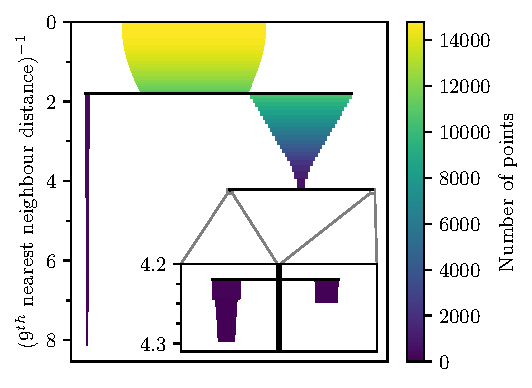
\includegraphics[width=0.7\textwidth]{fig/c2/fig_hdbscan.pdf}
   \caption[Condensed tree graph for HDBSCAN with $m_{clSize}=80$ applied to a $2.5^{\circ}$ field around Blanco 1]{Condensed tree graph for HDBSCAN with $m_{clSize}=80$ applied to a $2.5^{\circ}$ field around Blanco 1, a nearby cluster without any other known OCs in the field. The colour and width of each icicle denotes the number of stars remaining in the cluster. Horizontal splits occur when clusters are no longer connected. The long icicle on the left is Blanco 1, which is an extremely clear, nearby cluster and hence splits early from field stars. On the right, the algorithm continues discarding field stars, splitting into two very short icicles at the end which are false positive clusters. The two small sub-plots in the lower right are zoomed in on the two small icicles.}\label{c2:fig:hdbscan}%
\end{figure}

HDBSCAN \citep{hutchison_hdbscan_2013} is a more recently developed clustering algorithm \review{that attempts to improve the performance and usability of previous approaches. HDBSCAN combines the density-based approach of DBSCAN with hierarchical clustering, allowing it to deal with datasets of varying densities. Despite the extra computations, HDBSCAN does not have a significant increase in runtime compared to DBSCAN. 
}

\review{To evaluate possible clustering, nearest neighbour distances are calculated }as with DBSCAN\review{. However, HDBSCAN then }effectively considers all possible DBSCAN solutions for all possible values of $\epsilon$, \review{constructing a hierarchical tree }representation of the \review{possible clusterings of the dataset. As }with DBSCAN, \review{clusters are defined using an $m_{Pts}$ parameter to define }core and border points. \review{HDBSCAN `replaces' the }$\epsilon$ \review{parameter of DBSCAN with a }minimum cluster size $m_{clSize}$\review{, which is used to define the minimum possible size of a cluster before all points within it are instead classified as noise}. Smaller values of $m_{clSize}$ cause the hierarchical graph to be split more, as deeper, more nested solutions become valid. Larger $m_{clSize}$ values will merge small groups, negating the algorithm's sensitivity to clusters smaller than $m_{clSize}$ but while reducing the number of \review{false positive }associations of points in the dataset that are reported as clusters.

Figure~\ref{c2:fig:hdbscan} shows a representation of the HDBSCAN hierarchical graph for clustering analysis performed on a 2.5$^\circ$ field centred on Blanco 1, with parameters $m_{clSize}=80$ and $m_{Pts}=10$. \review{Having produced a hierarchical graph representation of the dataset, clusters }can be selected \review{from it }in one of two ways. In the Excess of Mass (EoM) method, the clusters with the largest area in this plot are selected. Alternatively, in the leaf method, more fine-grained structure is revealed, as clusters at the bottom of the tree are always selected. 

HDBSCAN solves a number of issues encountered by previous approaches in the literature. For instance: whereas DBSCAN requires setting the $\epsilon$ parameter homogeneously across an entire dataset, giving it poor performance when detecting clusters of different densities, HDBSCAN's consideration of all DBSCAN solutions simultaneously gives it equal sensitivity across all density ranges of a dataset. \review{In addition, $m_{clSize}$ is a much more intuitive parameter to set than $\epsilon$ for detecting OCs, since the minimum allowable size of an OC can be decided beforehand and does not require an additional method to try and estimate it for a given dataset as with $\epsilon$.
}

However, use of HDBSCAN comes with some challenges when running on largely unclustered data - such as the \emph{Gaia} dataset, where very few stars reside in OCs. HDBSCAN is sensitive to all regions of a dataset where points appear statistically more clustered than the local background, particularly when setting the parameter $m_{clSize}$ low to ensure that HDBSCAN is sensitive to the smallest galactic OCs. In the \emph{Gaia} regime, it is unsurprising that a field of one million stars will contain many low signal to noise ratio false positive associations, where groups of 10$-$20 stars will appear more clustered than the background by statistical chance. These false positives will be reported by HDBSCAN and must be later removed to use HDBSCAN successfully at high sensitivities.

The Python implementation of HDBSCAN by \cite{mcinnes_hdbscan_2017} was used for this work, which differs from the original publication in a few small ways (such as using a $k$-d tree for nearest neighbour computation) that allow the algorithm to run faster. 

\subsubsection{Parameter tuning}

HDBSCAN parameters were straightforward to set in a number of small experiments conducted on well-characterised OCs. While the original HDBSCAN paper recommends setting $m_{Pts}$ and $m_{clSize}$ to the same value, setting $m_{Pts}=10$ was found to offer the best sensitivity and speed when running the algorithm, a decision also supported by the arguments for setting $m_{Pts}=10$ for DBSCAN.

To select candidate clusters from the hierarchical tree, the leaf selection method was almost always superior to the EoM method. OCs contain a very small number of stars ($\sim$100) compared to the fields they occupy ($\sim$100 000+), and the leaf selection method was significantly better at recovering the smallest objects (OCs) in a given field.

However, there is no perfect setting for $m_{clSize}$ \review{having investigated the effect of the parameter in a number of small experiments, for which we tested different parameter values against a representative set of OCs. An exact $m_{clSize}$ setting must be found empirically based on the properties of a dataset. While theory suggests that $m_{clSize}$ should not be smaller than the smallest size of an OC (which we define as ten stars in this work), such low values were found to produce }a large number of false positives\review{, also }sometimes erroneously splitting the largest OCs into two or more sub-clusters that miss many valid members of the cluster. Alternatively, setting it high (e.g. $m_{clSize}=80$) makes the algorithm's output significantly less noisy at the cost of missing the smallest objects. \review{Values larger than 80 had no added advantages despite further decreasing the algorithm's sensitivity to smaller OCs. }High values also sometimes select dense regions of field stars that must be removed later as they are not OCs.  They may correspond to moving groups such as those reported by \cite{kounkel_untangling_2019} and \cite{kounkel_untangling_2020}. A range of settings (10, 20, 40 and 80) will be compared in this paper. 


%--------------------------------------------------------------------


\subsection{Gaussian mixture models}

\subsubsection{Description of algorithm}

GMMs differ from the other methods considered in this study in a number of ways, offering an interesting alternative viewpoint on how an entirely different and much older method performs when trying to detect OCs in a large, modern dataset. The data are assumed to be drawn from a number of Gaussian distributions, to which the algorithm fits a mixture of $m$ Gaussian components across a series of iterations. The likelihood of consecutive iterations is maximised until convergence is achieved. Covariances between dimensions allow the fitted Gaussians to have an elliptical or diagonal shape, which is important for OCs as many are elongated due to tidal effects.

Since all points must be assigned as a member of a Gaussian, GMMs do not have a natural way to deal with unclustered field stars. Instead, mixture components must be ruled out if their properties are incompatible with OCs. The means and standard deviations of mixture components in the different scaled dimensions $(\lambda, \, \phi, \, \mu_{\lambda*}, \, \mu_{\phi}, \, \varpi)$ can be quickly used as proxies for the properties of a candidate OC, with any targets wholly incompatible with an OC ruled out as groupings of field stars. We adopt a similar approach to \cite{cantat-gaudin_gaia_2019} and require that the following constraints are met on the proper motion dispersion $(\sigma_{\mu_{\lambda*}}, \, \sigma_{\mu_{\phi}})$ and the dispersion in positional space $(\sigma_{\lambda}, ,\ \sigma_{\phi})$ respectively:

% Proper motion constraint
\begin{equation}
\sqrt{\sigma_{\mu_{\lambda*}}^2+\sigma_{\mu_{\phi}}^2} \leq
  \begin{cases}
    1 \text{ mas yr}^{-1}                  & \varpi \leq 0.67 \text{ mas} \\
    1.49 \cdot \varpi \text{ mas yr}^{-1}  & \varpi >    0.67 \text{ mas} \\
  \end{cases} 
\end{equation}

% Radius constraint
\begin{equation}
\sqrt{\sigma_{\lambda}^2+\sigma_{\phi}^2} \leq
  \begin{cases}
    0.1 ^{\circ}                  & \varpi \leq 0.17 \text{ mas} \\
    \arctan(\varpi / 100)^{\circ} & \varpi >    0.17 \text{ mas} \\
  \end{cases} 
\end{equation}

\noindent
which differs from the constraints of \cite{cantat-gaudin_gaia_2019}, who only include a proper motion constraint. The addition of a latter radius constraint helps to remove clear false positives that are significantly larger than the typical size of OCs.

The implementation of GMMs freely available in \texttt{scikit-learn} \citep{pedregosa_scikit-learn_2011} was used in this study. In addition, \cite{cantat-gaudin_gaia_2019} have used UPMASK \citep{krone-martins_upmask:_2014} to verify OC candidates. However, this was deemed unnecessary for this study, as the sample of OC candidates after the application of the constraints was already relatively clean with few false positives.

\begin{figure}[t]
   \centering
   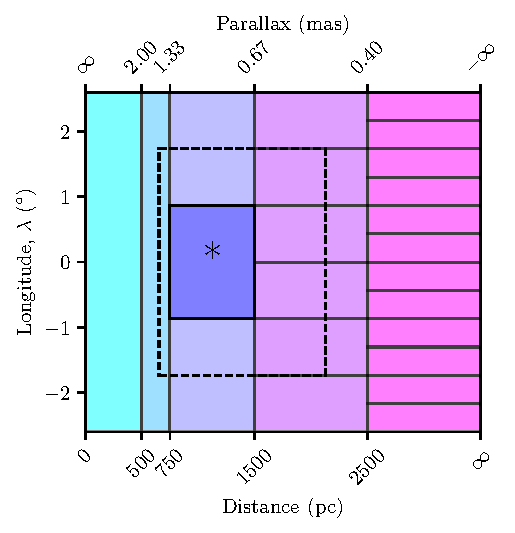
\includegraphics[width=0.7\textwidth]{fig/c2/fig_gmm.pdf}
   \caption[Schematic, top-down representation of the GMM partitioning system]{Schematic, top-down representation of the GMM partitioning system. Each box represents a column of sub-partitions viewed from the top. For the highlighted sub-partition also marked with an asterisk (*), the dashed width of the box shows the region in which extra stars with a parallax uncertainty of greater than 1 mas would be included. The height of the dashed box shows the extra overlap between this sub-partition and nearby other sub-partitions. Any cluster with a centroid within the dashed region but not within the main highlighted region was automatically discarded, as it will be better characterised by the neighbouring sub-partition its centroid is in.}\label{c2:fig:gmm}%
\end{figure}

\subsubsection{Parameter tuning \& dataset sub-partitioning}

Issues were encountered when attempting to tune the number of mixtures $m$. Firstly, larger fields required linearly more mixtures to ensure that enough were available for fitting to field stars, such that $m \propto n$. Instead, it is easier to set the parameter $m_s$, the number of stars per mixture -- where $m = n / m_s$. This causes the method to be $n$ times slower, since the GMM runtime complexity also scales linearly with the number of mixtures $\mathcal{O}(nm)$, which for this choice of parameters means it is equivalent to $\mathcal{O}(n^2)$ since the number of mixtures linearly increases with the number of stars. This causes the method to fail the speed criterion (criterion one) from Sect.~\ref{c2:sec:algorithms_criteria}, even though it was initially believed to be the fastest method under consideration.

To rectify this and ensure that GMMs can still be included in this study, a method for sub-partitioning \emph{Gaia} data chunks was devised. While \cite{cantat-gaudin_gaia_2019} used a $k$-d tree to partition fields into groups of 8000 stars, this method had no overlap between partitions, and hence may miss OCs that are split between partitions. $k$-d trees work by splitting random dimensions of a dataset along their median until each branch of the tree is small enough, a process that has no guarantee against splitting a possible OC into many different branches.

Instead, stars in a given field were divided into five segments based on parallax, where stars may be a member of any segment that they have a better than $2\sigma_{\varpi}$ agreement with. Each parallax segment was sub-divided into smaller HEALPix pixels at a specific level. Neighbouring HEALPix pixels were also selected to overlap sub-partitions between each other. The levels of the primary and overlap pixels were carefully selected to ensure that the nearest edge of every sub-partition could always fully contain an OC of 10 pc radius. In the case of the most diffuse OCs, this method could miss some stars that are far from the OC's centre, but should always be able to detect the core of all OCs. When any sub-partition in a parallax range contained fewer than $10m_s$ stars, the main HEALPix level for the parallax segment was decreased by one to increase the number of stars in the sub-partitions. This ensured that no sub-partition was impractically small for later GMM fitting. A schematic representation of this is shown in Fig.~\ref{c2:fig:gmm}, and the values for the sub-partitions are listed in Table~\ref{c2:tab:gmm_parameters}.

\begin{table}
\caption[Specifications of the GMM sub-partitioning scheme]{Specifications of the GMM sub-partitioning scheme.}
\label{c2:tab:gmm_parameters}
\centering
\begin{tabular}{c c c c}
\hline\hline
distance       & Max. HEALPix    & Max. sub & Optimum \\
range (pc)     & level (overlap) & partitions\tablefootmark{a} & $m_s$   \\
\hline                        
0 - 500         & None (None) & 1   & 1000 \\ 
500 - 750       & None (None) & 1   & 1000 \\
750 - 1500      & 5    (6)    & 9   & 800  \\
1500 - 2500     & 6    (7)    & 36  & 600  \\
2500 - $\infty$ & 7    (8)    & 144 & 250  \\
\hline

\end{tabular}

\tablefoot{
\tablefoottext{a}{When fewer than $10m_s$ stars were in a sub-partition, the main HEALPix level was decreased by one to make the sub-partitions a factor of four larger.}
}

\end{table}


Any OC candidate with a centroid $(\lambda, \, \phi)$ in an overlap pixel is automatically discarded, as it is assumed to be better characterised in the neighbouring sub-partition for which it would be more fully selected. The sub-partitioning scheme improved the runtime of the method by a factor of about five and the memory use by a factor of about 80. This could be improved further by reducing the pixel sizes or overlap levels, albeit at the cost of sensitivity to OCs on the boundaries between sub-partitions.

Two scenarios were tested in this study for a value of $m_s$. Firstly, $m_s$ was fixed to 800 stars per mixture component, which was found to be a good general value across the entire dataset. Secondly, $m_s$ was varied depending on the parallax range, as in Table~\ref{c2:tab:gmm_parameters}. This was found to greatly improve the sensitivity of the method at high distances where OCs have fewer visible stars in \emph{Gaia} data and are much smaller.

Since GMMs are a method that relies on convergence, the randomly selected starting parameters of the Gaussian mixtures can affect the final result found by the method. Selecting the best result after multiple initialisations was not found to significantly improve results, so the \texttt{n\_init} parameter of the \texttt{scikit-learn} implementation was left at 1. However, the maximum number of iterations of the method, \texttt{max\_iter}, was set to 1000, to ensure that the method was always able to converge.




%--------------------------------------------------------------------

\section{Analysis}\label{c2:sec:results}
\subsection{Evaluation criteria for clustering algorithms}

So far, we prepared \emph{Gaia} data for clustering analysis, selected three algorithms for further study, and developed techniques to optimise them for use on \emph{Gaia} data. In this section, we explain how we quantify the performance of the algorithms against each other by crossmatching to existing objects in the literature, and we present those results.

We quantify the performance of the algorithms using \review{a number of standardised statistics. For our existing literature OCs, we expect that a number of them are real, or true positives }(TP)\review{. However, literature catalogues such as MWSC have been shown to have a number of erroneous entries \citep{cantat-gaudin_clusters_2020}, which are in reality true negatives }(TN)\review{. While a perfect algorithm would report all true positive OCs, missed objects are defined as false negatives (FN). Similarly, when a putative object is erroneously reported as real, it is defined as a false }positive (FP).

\review{It is convenient to use these quantities to derive performance statistics normalised to be between 0 and 1, and so we }also derive the sensitivity, specificity and precision of the algorithms, which are defined as:

\begin{equation}
    \text{Sensitivity} = \frac{\text{TP}}{\text{TP} + \text{FN}},
\end{equation}

\begin{equation}
    \text{Specificity} = \frac{\text{TN}}{\text{TN} + \text{FP}},
\end{equation}

\begin{equation}
    \text{Precision} = \frac{\text{TP}}{\text{TP} + \text{FP}}.
\end{equation}

\noindent
\review{Effectively, the sensitivity is a measure of an algorithm's ability to detect real objects, the specificity is its ability to reject putative objects, and the precision is the fraction of reported objects that the user could expect are actually real.} It follows that a perfect algorithm would have all three quantities at 1, since FN and FP would be zero. However, this is of course unrealistic as no algorithm is likely to be perfect, and different studies may wish to prioritise different statistics over one another. For instance, a search for new OCs would wish to use an algorithm with a maximised sensitivity, such that as many new OCs as possible could be discovered -- although the precision of such a study is also of concern, so that as few false positive OCs as possible are reported. A search for existing OCs that attempts to improve the general quality of the OC census would need to maximise all three quantities, and may be especially concerned with maximising the specificity of the method used, such that as many putative literature OCs as possible can be ruled out.

We look in detail at the 100 main OCs of this study and derive sensitivity, specificity and precision statistics for all algorithms in these cases, giving the usefulness of each algorithm and parameter combination when searching for a given literature OC. Then, in the second part of our results, we derive true positive rates for all algorithms across all OCs in the fields in this study, giving supplementary information on the sensitivity of each algorithm as a function of the reported literature distance and size of the OCs.


\subsection{False positive identification}\label{c2:sec:false_positives}

It is likely impossible to maximise both the specificity and sensitivity of any algorithm simultaneously: for all algorithms studied, increasing their sensitivity would always decrease their specificity. The detection of more true positive OCs always also resulted in more false positive OCs. We explore two techniques to reduce the number of false positives of the algorithms: firstly, by dropping all OC candidates with parameters unrealistic for an OC, and secondly, by using a density-based criterion to discard OC candidates that have a density compatible with being drawn from unclustered local field stars.

To reduce the number of false positive crossmatches -- particularly since algorithms such as HDBSCAN and DBSCAN when ran at maximum sensitivity reported over 40$\,$000 OC candidates, the majority of which are false positives -- OC candidates with mean parameters extremely incompatible with a real OC were first removed, using criteria presented in \cite{cantat-gaudin_clusters_2020}. The proper motion dispersion of OC candidates was required to satisfy

% Proper motion constraint
\begin{equation}\label{c2:eqn:proper_motion}
\sqrt{\sigma_{\mu_{\alpha*}}^2+\sigma_{\mu_{\delta}}^2} \leq
  \begin{cases}
    1 \text{ mas yr}^{-1}                  & \varpi \leq 0.67 \text{ mas} \\
    1.49 \cdot \varpi \text{ mas yr}^{-1}  & \varpi >    0.67 \text{ mas.} \\
  \end{cases} 
\end{equation}

\noindent
The radius containing half of the members of the OC candidate was also required to satisfy $r_{50} < 20$ pc. These constraints were relatively weak, only removing a small number of clearly anomalous OC candidates that had velocity dispersions or radii that were clearly incompatible with real OCs.

\begin{figure}[t]
   \centering
   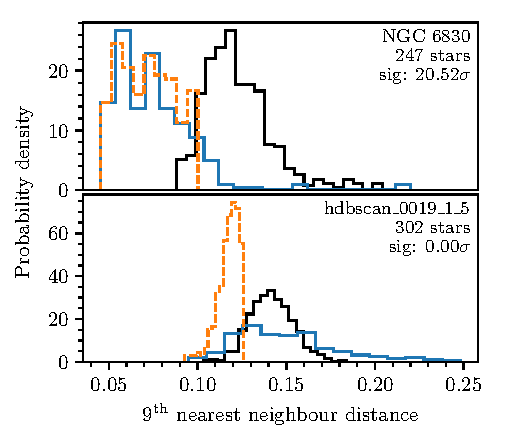
\includegraphics[width=0.7\textwidth]{fig/c2/fig_nn_distances.pdf}
   \caption[Two examples of NNDs used to test the significance of OC candidates]{Two examples of NNDs used to test the significance of OC candidates. The solid black line shows the NND of nearby field stars. The blue line shows the NND of distances between cluster members. For a cluster to be significant and not simply a selection of unclustered field stars, the cluster NND must be incompatible with being drawn from the field distribution. For later illustrative purposes, the NND of a cluster member to the nearest field star is shown by the dashed orange line, although this is not used for the CST. In the upper plot, an OC candidate detected by HDBSCAN and crossmatched to the well-characterised OC NGC 6830 is shown, which has a clearly different NND to field stars with a significance of over 20$\sigma$. In the lower plot, a false positive OC detected by HDBSCAN in field 19 is shown that has a significance of 0$\sigma$.}\label{c2:fig:nn_distances}%
\end{figure}

Secondly, a method was implemented to compare the density of OC candidates with the density of local field stars and evaluate the significance of the OC candidate, hence referred to as the cluster significance test (CST). Ninth nearest neighbour distances between stars were used as a proxy for density, as this corresponds exactly to how two of the three methods in this study performed clustering analysis (since they used $m_{Pts}=10$, i.e. $k=9$) and since this value is free of contamination from binary or multiple star systems, since they will have significantly smaller first or second nearest neighbour distances.

To calculate the density distribution of a cluster, the nearest neighbour distribution (NND) of intra-cluster distances between stars within an OC candidate was calculated. Then, in an iterative approach, a minimum of 100 and a maximum of 500 local field stars were found around the OC candidate by traversing the graph of nearest neighbours and looking for field stars with NNDs uncontaminated by proximity to the cluster, meaning that none of their $1^\text{st}$ to $9^\text{th}$ nearest neighbours were labelled as cluster members. This approach was found to generate reliable and quick approximations of the NND of local field stars.

Since a good OC candidate is a clear overdensity in the parameter space, its NND should be incompatible with being drawn from the distribution of field stars. A number of statistical tests were investigated to test this, with a Mann-Whitney U test \citep{mann_test_1947} found to be the most reliable, since it makes no assumptions about the shape of the distribution and does not require the distribution to be continuous. Significance values for each OC candidate are then derived from a one-tailed test where the alternate hypothesis is that the OC candidate has an NND incompatible with and with a lesser median than the field NND.

Requiring a CST value of at least 3$\sigma$ was found to keep the vast majority of good OCs while identifying and removing a large number of false positives for all algorithms. For instance, for DBSCAN when running with $\epsilon_{n3}$ (the algorithm and parameter combination that produced the highest number of OC candidates), the CST constraint reduced the number of reported OC candidates from 51920 to just 1111 objects.


\subsection{Crossmatches with existing catalogues}\label{c2:sec:results_crossmatch}

Having greatly reduced the number of false positives identified by all algorithms, we crossmatched OC candidates against literature clusters to estimate the number of true positives detected by each algorithm. However, this process is non-trivial, with each catalogue reporting OCs in different ways.

A number of approaches were trialed to crossmatch OC candidates. The best approach found to crossmatch OC candidates' positions was that of \cite{liu_catalog_2019}. The tidal radius of OC candidates is estimated as the maximum distance of a member star from its mean $\alpha$ and $\delta$. The OC candidate must be within one tidal radius of the reported position in the literature, where whichever tidal radius is larger (that of the candidate or that of the literature cluster) is used. This would typically correspond to searching in a radius of no more than $0.5^\circ$.

$\mu_{\alpha*}$, $\mu_{\delta}$ and $\varpi$ for OC candidates were required to be within $5 \sigma$ (5 standard errors) of literature values. It has been shown that \emph{Gaia} DR2 has a number of small unaccounted for systematic effects, including a parallax zero-point offset $\varpi_0$ that may be magnitude-dependent \citep{lindegren_gaia_2018}. As such, even when crossmatching to other OCs detected in \emph{Gaia} data, magnitude-dependent systematic errors could cause crossmatches to fail. For instance, \cite{castro-ginard_hunting_2020} have only studied \emph{Gaia} data to $G=17$. Extra stars introduced by this study using a magnitude cut of $G=18$ will have a different mean systematic effect on derived astrometric parameters. Additionally, every clustering algorithm will report slightly different membership lists for each OC, and the differences in parameters of included or ignored members could introduce different systematic errors. In ($\alpha$, $\delta$), these effects are small, since tidal radii (often no smaller than $\sim0.1^{\circ}$) are much larger than the small systematic errors in position of the \emph{Gaia} reference frame. However, large OCs especially may have standard errors on their mean parallax or proper motion as small as $10$ $\mathrm{\mu}$as or $10$ $\mathrm{\mu}$as yr$^{-1}$, smaller than the reported \emph{Gaia} systematic errors.

To rectify missed crossmatches, small tolerances to uniform systematic errors of 50 $\mathrm{\mu}$as yr$^{-1}$ and 50 $\mathrm{\mu}$as were accounted for in crossmatching of proper motions and parallaxes respectively. These values were selected to roughly account for the scatter in parallax and proper motion offsets as a function of magnitude as reported by \cite{lindegren_gaia_2018}. This allowed a number of larger OC candidates with very small uncertainties \citep[particularly from the catalogue of][]{cantat-gaudin_clusters_2020} to be successfully crossmatched. Many of these large OC candidates were visible by eye in the \emph{Gaia} data and in the reported results of the clustering algorithms, and were being missed in the crossmatch procedure by a lack of tolerance to systematic error and due to their small uncertainties on parameters owing to their large size.

As the only non- \emph{Gaia}  catalogue, MWSC was more complicated to crossmatch against. Reported distances to OCs were converted to parallaxes. While distance measurements in MWSC do not include uncertainties, the estimated 11\% systematic uncertainty on distance measurements reported by \cite{kharchenko_global_2013} was accounted for. A parallax offset of $\varpi_0 = -0.029$ mas was applied to MWSC parallaxes, ensuring that they have the same mean systematic offset as parallaxes in the \emph{Gaia} DR2 dataset as reported by \cite{lindegren_gaia_2018}. The additional $\pm$0.8 mas yr$^{-1}$ external error in MWSC proper motions was also accounted for, which resulted in a handful of extra crossmatches to objects clearly crossmatched in other dimensions that had large offsets in their proper motions relative to \emph{Gaia} DR2.


\subsection{Results}\label{c2:sec:analysis_results}

Finally, we present analysed results of the algorithms for discussion in three parts.

Firstly, we inspected \emph{Gaia} data manually to assign the 100 main OCs as either true positives or true negatives. An interactive data viewer was used to explore the region around the reported locations of the OCs, searching for significant overdensities within the possible crossmatch region. We also required that the detected overdensity had a colour magnitude diagram (CMD) compatible with an OC, for which we define the following criteria.

A class one OC has a clear, difficult to dispute CMD, with a realistic shape. The CMD may be somewhat broadened by differential extinction or inhomogeneities, but there should be enough stars present to make the probability of a false alarm very small. However, a class two OC is a possible OC that may be too small or too inhomogeneous for its true existence to be clear. It may be that only the brightest stars (near the turnoff point) are detected, making its shape difficult to discern as a true isochrone. There may be a small number of outlier stars incompatible with an isochrone, owing to a poor detection by the algorithm. This class signifies that more work would be needed to confirm this object as an OC. Finally, class three OCs are very unlikely to be an OC and much more compatible with random noise. Even if some stars follow an isochrone, a significant number are outliers, owing to this being a selection of unclustered, inhomogeneous stars.

After an overdensity was isolated in position, proper motion and parallax, it was required to have a class one or two CMD to confirm it as a true positive OC. We assigned 40 OCs as true positives and the remaining 60 as true negatives.

31 of the 33 OCs in the list of main OCs from MWSC that are also in the catalogue of \cite{cantat-gaudin_clusters_2020} were entered as true positives. Most of these objects were good OCs that were clearly visible at their reported location. We did not detect significant overdensities with class one or two CMDs corresponding to Patchick 75 or Auner 1, both of which are distant OCs with distances in \cite{cantat-gaudin_clusters_2020} of $\sim$7 kpc and $\sim$8 kpc respectively. These OCs are heavily polluted in the literature membership lists. If real, they are scarcely detectable in \emph{Gaia} data. Alternatively, they may simply not be real objects.

Most of the additional 67 OCs listed in MWSC do not appear detectable in \emph{Gaia} data, and may simply not be real objects. However, we did find sparse overdensities corresponding to nine objects from MWSC: ASCC 28, ASCC 100, ASCC 130, BDSB 124, Berkeley 64, DBSB 164, IRAS 06046-0603, SAI 90 and Teutsch 146. 

After reducing the number of false positives in the results of the algorithms using the techniques from Sect.~\ref{c2:sec:false_positives}, we crossmatched their results to the main list of 100 OCs and derived performance statistics. To quantify uncertainty on derived statistics, we used the method for computing Bayesian binomial confidence intervals described in \cite{cameron_estimation_2011}, where a Beta distribution with an uninformative prior is used to estimate a confidence interval containing the true success fraction given the measured success fraction. The performance of the algorithms is listed in Table~\ref{c2:table:classifications}. 

Five OCs from the 40 true positives are never detected by any algorithm within our constraints, which we discuss here for completeness: Berkeley 91 and Teutsch 156 \citep[objects from][]{cantat-gaudin_clusters_2020} as well as ASCC 28, BDSB 124 and Teutsch 146 from MWSC. Berkeley 91 is relatively distant ($\sim4$ kpc) OC with a polluted CMD in the catalogue of \cite{cantat-gaudin_clusters_2020}. If real, it is barely detectable in \emph{Gaia} data. Teutsch 156 appears to be detected by HDBSCAN, but only tentatively with a CST of 0.68$\sigma$. ASCC 28 should be detected, as the detected overdensity was nearby with a parallax of 0.85 mas. It may be too sparse for an algorithm to detect or may be an association mis-classified by the expert classifier. The BDSB 124 and Teutsch 146 overdensities are distant ($\varpi \approx 0.3$ mas and 0.25 mas respectively) with polluted CMDs. These objects may be difficult for algorithms to detect in \emph{Gaia} data or may simply be associations.

\review{Six OCs from MWSC listed as true negatives are reported at some point by any algorithm (five by HDBSCAN, two by DBSCAN), although only OC candidates crossmatched to FSR 0316 are detected by two different algorithms (HDBSCAN and DBSCAN). In all of these cases, the objects are sparse and relatively separated from the reported literature locations on the sky, and may be new OCs that marginally coincide with the existing locations.
}

Secondly, we performed crossmatches to all \review{1385 }targets listed in the literature in the fields of this study. While there are too many OCs to conduct a precise by-hand treatment of the results, these results give a better indication of the dependence of the algorithms' sensitivities on OC features like distance, age and size. \review{Clear dependencies on distance and size are found, which are shown in Fig.~\ref{c2:fig:detections_by_distance}. }No significant dependence on ages listed in MWSC is found for any of the algorithms, \review{although the more recent and accurate age catalogue of 
\cite{cantat-gaudin_painting_2020} did reveal a slight dependence on age that appears to result from the smaller size of older OCs. HDBSCAN is the most sensitive algorithm across all ages. When combining all $\epsilon$ runs, DBSCAN is as sensitive for well populated young OCs, but is less sensitive to older, typically smaller OCs. GMMs are the worst algorithm across all ages.
}

Finally, to compare the general usability of the algorithms, we list the runtimes and the total number of OC candidates with valid proper motion dispersions and radii reported by each algorithm in Table~\ref{c2:tab:algorithm_performance}. Ideally, an algorithm would report a realistic number of OC candidates in as little time as possible.

We also list additional comparisons of our results with other catalogues in Appendix~\ref{app:c2:comparison_with_cats}. \review{Full tables of detected and non-detected objects (including OC membership lists) are available in the online material only, with descriptions of their content in Appendix~\ref{app:c2:extra_tables}.
}


% Table showing detections as a fn of class
\begin{sidewaystable}[p]
\caption[Performance of different algorithm and parameter combinations on the 100 main OCs]{Performance of different algorithm and parameter combinations on the 100 main OCs.}              % title of Table
\label{c2:table:classifications}      % is used to refer this table in the text
\centering                                      % used for centering table
\begin{tabular}{l l | c c c c | c c c}          % centered columns (4 columns)
\hline\hline                        % inserts double horizontal lines

Algorithm & Parameters & TP & FP & TN & FN & Sensitivity & Specificity & Precision \\    
\hline
DBSCAN    & $\epsilon_{ACG}$, 1 repeat   & 22 $^{25.0}_{18.8}$ & 0 $^{1.8}_{0.0}$ & 60 $^{60.0}_{58.2}$ & 18 $^{21.2}_{15.0}$ & 0.55 $^{0.62}_{0.47}$ & 1.00 $^{1.00}_{0.97}$ & 1.00 $^{1.00}_{0.91}$ \rule{0pt}{0.35cm}\\[0.1cm]
$\quad$-  & $\epsilon_{ACG}$, 30 repeats & 20 $^{23.1}_{16.9}$ & 0 $^{1.8}_{0.0}$ & 60 $^{60.0}_{58.2}$ & 20 $^{23.1}_{16.9}$ & 0.50 $^{0.58}_{0.42}$ & 1.00 $^{1.00}_{0.97}$ & 1.00 $^{1.00}_{0.90}$ \\[0.1cm]
$\quad$-  & $\epsilon_{c}$               & 20 $^{23.1}_{16.9}$ & 1 $^{3.2}_{0.7}$ & 59 $^{59.3}_{56.8}$ & 20 $^{23.1}_{16.9}$ & 0.50 $^{0.58}_{0.42}$ & 0.98 $^{0.99}_{0.95}$ & 0.95 $^{0.97}_{0.84}$ \\[0.1cm]
$\quad$-  & $\epsilon_{n1}$              & 20 $^{23.1}_{16.9}$ & 0 $^{1.8}_{0.0}$ & 60 $^{60.0}_{58.2}$ & 20 $^{23.1}_{16.9}$ & 0.50 $^{0.58}_{0.42}$ & 1.00 $^{1.00}_{0.97}$ & 1.00 $^{1.00}_{0.90}$ \\[0.1cm]
$\quad$-  & $\epsilon_{n2}$              & 7 $^{10.0}_{5.2}$ & 2 $^{4.5}_{1.4}$ & 58 $^{58.6}_{55.5}$ & 33 $^{34.8}_{30.0}$ & 0.17 $^{0.25}_{0.13}$ & 0.97 $^{0.98}_{0.93}$ & 0.78 $^{0.88}_{0.54}$ \\[0.1cm]
$\quad$-  & $\epsilon_{n3}$              & 2 $^{4.4}_{1.3}$ & 0 $^{1.8}_{0.0}$ & 60 $^{60.0}_{58.2}$ & 38 $^{38.7}_{35.6}$ & 0.05 $^{0.11}_{0.03}$ & 1.00 $^{1.00}_{0.97}$ & 1.00 $^{1.00}_{0.43}$ \\[0.1cm]
$\quad$-  & $\{ \epsilon_{c}, \, \epsilon_{n1}, \, \epsilon_{n2}, \, \epsilon_{n3} \} $ & 25 $^{27.8}_{21.8}$ & 2 $^{4.5}_{1.4}$ & 58 $^{58.6}_{55.5}$ & 15 $^{18.2}_{12.2}$ & 0.62 $^{0.69}_{0.54}$ & 0.97 $^{0.98}_{0.93}$ & 0.93 $^{0.95}_{0.83}$ \\[0.1cm]

\hline

HDBSCAN   & $m_{clSize} = 80$            & 17 $^{20.2}_{14.1}$ & 3 $^{5.7}_{2.1}$ & 57 $^{57.9}_{54.3}$ & 23 $^{25.9}_{19.8}$ & 0.42 $^{0.50}_{0.35}$ & 0.95 $^{0.97}_{0.91}$ & 0.85 $^{0.91}_{0.71}$ \rule{0pt}{0.35cm}\\[0.1cm]
$\quad$-  & $m_{clSize} = 40$            & 24 $^{26.8}_{20.8}$ & 6 $^{9.2}_{4.4}$ & 54 $^{55.6}_{50.8}$ & 16 $^{19.2}_{13.2}$ & 0.60 $^{0.67}_{0.52}$ & 0.90 $^{0.93}_{0.85}$ & 0.80 $^{0.86}_{0.69}$ \\[0.1cm]
$\quad$-  & $m_{clSize} = 20$            & 31 $^{33.1}_{27.9}$ & 7 $^{10.3}_{5.2}$ & 53 $^{54.8}_{49.7}$ & 9 $^{12.1}_{6.9}$ & 0.78 $^{0.83}_{0.70}$ & 0.88 $^{0.91}_{0.83}$ & 0.82 $^{0.86}_{0.73}$ \\[0.1cm]
$\quad$-  & $m_{clSize} = 10$            & 33 $^{34.8}_{30.0}$ & 7 $^{10.3}_{5.2}$ & 53 $^{54.8}_{49.7}$ & 7 $^{10.0}_{5.2}$ & 0.82 $^{0.87}_{0.75}$ & 0.88 $^{0.91}_{0.83}$ & 0.82 $^{0.87}_{0.74}$ \\[0.1cm]

\hline

GMM       & $m_{s} = 800$                & 7 $^{10.0}_{5.2}$ & 0 $^{1.8}_{0.0}$ & 60 $^{60.0}_{58.2}$ & 33 $^{34.8}_{30.0}$ & 0.17 $^{0.25}_{0.13}$ & 1.00 $^{1.00}_{0.97}$ & 1.00 $^{1.00}_{0.75}$ \rule{0pt}{0.35cm}\\[0.1cm]
$\quad$-  & $m_{s} = $ variable          & 13 $^{16.2}_{10.4}$ & 0 $^{1.8}_{0.0}$ & 60 $^{60.0}_{58.2}$ & 27 $^{29.6}_{23.8}$ & 0.33 $^{0.41}_{0.26}$ & 1.00 $^{1.00}_{0.97}$ & 1.00 $^{1.00}_{0.85}$ \\[0.1cm]



\hline                                             %inserts single line
\end{tabular}

\tablefoot{True positive (TP), false positive (FP), true negative (TN) and false negative (FN) counts of detected clusters are given along with the sensitivity, specificity and precision. 68.3\% confidence intervals are shown for all numbers. Confidence intervals for a handful of values (e.g. measured precisions of exactly 0.0 or 1.0) were adjusted to include the measured values. This corrects for approximations in the calculation of binomial confidence intervals where the measured success probability is exactly 0 or 1. All objects that did not pass the criterion in Sect.~\ref{c2:sec:false_positives} with a CST greater than 3$\sigma$ were discarded before crossmatching and producing this table.}

\end{sidewaystable}

% Detections vs. distance and size
\begin{figure}[ht]
   \centering
   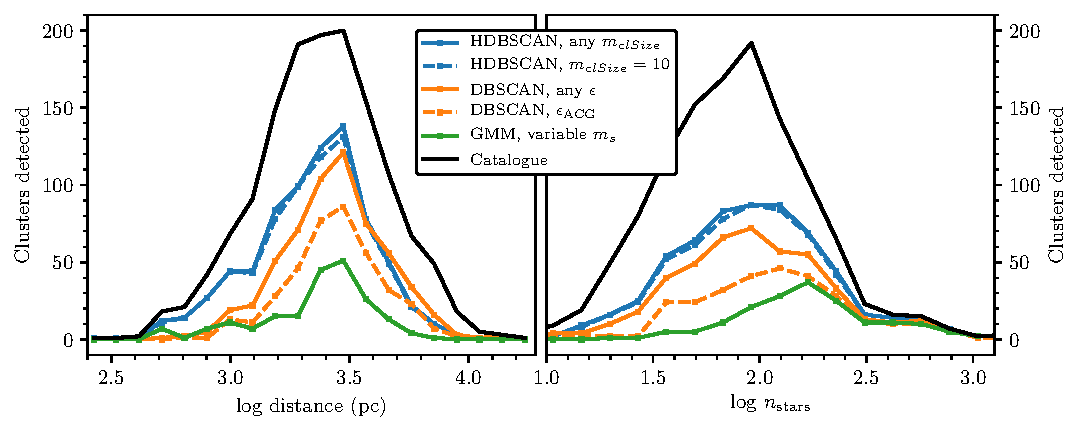
\includegraphics[width=\textwidth]{fig/c2/fig_crossmatches.pdf}
   \caption[Distance and size dependence of detections by different algorithm and parameter combinations for all 1385 OCs in all studied fields]{Distance and size dependence of detections by different algorithm and parameter combinations for all  \review{1385 }OCs in all studied fields, plotted against the reported size and distance of the OCs in the literature. OC candidates not passing the criterion in Sect.~\ref{c2:sec:false_positives} and with a CST of less than 3$\sigma$ were discarded. HDBSCAN detects the most OCs, especially at nearby distances. GMMs only perform well at detecting well populated OCs. While individual DBSCAN results at different $\epsilon$ values do not detect especially many OCs, combining them all together nearly matches the performance of HDBSCAN -- even exceeding it slightly at large distances.}\label{c2:fig:detections_by_distance}%
\end{figure}

%DIF >  Table with extra information about runtimes etc
\begin{sidewaystable}[p]
\caption[Extra information on the algorithms' performance]{\review{Extra information on the algorithms' performance.}}
\label{c2:tab:algorithm_performance}
\centering
\begin{tabular}{l c c c c}
\hline\hline
Algorithm& Reported OC candidates\tablefootmark{a} & \review{Fraction with CST > $3\sigma$ }& \review{Total crossmatches}\tablefootmark{b} & Mean runtime (mins)\tablefootmark{c} \\
\hline

DBSCAN (ACG)    & 1518 to 1538  & \review{58.9\% to 59.6\%} & \review{382 }& \begin{tabular}{@{}l@{}}\review{1.19 (1 repeat) to }\\ 10.3 (30 repeats)\end{tabular}       \\[0.25cm]

DBSCAN (model)  & 5212 to 51920 & \review{22.4\% to 2.1\%}  & \review{593 }& 0.885 \\[0.1cm]

HDSBCAN         & 1196 to 49693 & \review{82.0\% to 5.2\%}  & \review{756 }& 2.36 \\[0.1cm]

GMM             & 314 to 2465   & \review{60.5\% to 20.5\%} & \review{213 }& \begin{tabular}{@{}l@{}}21.9 ($m_s=800$) \\ 47.0 (variable $m_s$)\end{tabular}      \\
\hline

\end{tabular}

\tablefoot{
\tablefoottext{a}{Total number of OC candidates for all fields that passed the proper motion dispersion and radius constraints from Sect.~\ref{c2:sec:false_positives}. The range is between the minimum and maximum reported number for the least and most sensitive parameters.}
\tablefoottext{b}{Total crossmatches is given as the union of all results from all parameter sets for a given method. A total of 1385 literature OCs were crossmatched against.}
\tablefoottext{c}{Mean runtime for a single field out of the 100 in this study. All runs were conducted on the same workbench computer with a 3.1 GHz 4-core CPU.}
}

\end{sidewaystable}





%--------------------------------------------------------------------
\section{Comparison of algorithms}\label{c2:sec:discussion}

Finally, having selected three algorithms for further study and having ran them on 100 representative fields across the galactic disk, we address the central topic of this work as to which clustering algorithm is best at detecting OCs in \emph{Gaia} data. We discuss the pros and cons of each algorithm in subsections before presenting an opinion.


\subsection{DBSCAN is effective at searching for OCs}

DBSCAN is a well proven algorithm on \emph{Gaia} data, having recently detected over 500 new OCs in \cite{castro-ginard_hunting_2020}. It performed relatively well on the 100 main OCs in this study. $\epsilon_\text{ACG}$ has particularly high specificity and precision values of $\approx1.00$ (Table~\ref{c2:tab:algorithm_performance}), suggesting that DBSCAN can produce consistent and reliable results when not ran sensitively. However, even when greatly increasing its theoretical sensitivity (e.g. $\epsilon_{n3}$, the highest $\epsilon$ value used in this study), DBSCAN still is not able to detect all OCs present in a field.

At individual values of $\epsilon$, Fig.~\ref{c2:fig:detections_by_distance} shows that DBSCAN is most sensitive to OCs at certain distances, with the $\epsilon_\text{ACG}$ sensitivity peaking at 3.1 kpc. This is likely due to how distant OCs are very compact in all dimensions, while nearby OCs in the sample may have radii of up to 0.5$^\circ$ or more, and are hence much sparser in the two positional dimensions and require the global density threshold $\epsilon$ to be higher for them to be completely detected. This is a key disadvantage of DBSCAN: single, global $\epsilon$ parameters rarely seem to be perfect for individual OCs, especially when the global parameter is influenced by density contributions from many different OCs in a single field. 

Manual comparison between algorithm results shows that DBSCAN often under or over-selects OCs and produces less reliable membership lists than HDBSCAN or GMMs. Over-selection is a particular issue as CMDs become polluted and the performance of OC candidates in the CST is reduced, as the nearest neighbour distribution becomes dominated by contaminating field stars. Many OC candidates detected by DBSCAN at CST values of less than 3$\sigma$ appear to correspond to real OCs, but are too polluted or too sparse to pass criterion to verify the candidate objects as real. In addition, these membership lists containing too few or too many members are of less use to other scientific applications, and would need to be followed up with another algorithm to improve their quality.

This can be partially mitigated by combining all DBSCAN results across all $\epsilon$ values, which approaches a similar degree of sensitivity to HDBSCAN, albeit still with a deficit of detections for small distances at less than 1 kpc. This result is in good agreement with what theory presented in Sect.~\ref{c2:sec:hdbscan} suggests: that a single run of DBSCAN's global density parameter will only be sensitive to a certain size of OC at a given distance, and that running HDBSCAN is equivalent to running DBSCAN across all possible values of $\epsilon$. However, HDBSCAN is better still -- able to detect the majority of OCs in the sample in a single run at $m_{clSize}=10$. 

Combining multiple DBSCAN results is similar to the effective approach that \cite{castro-ginard_hunting_2020} use to detect over 500 new OCs, since they vary the $m_{Pts}$ parameter and the size of the field analysed by the algorithm. $\epsilon_{\text{ACG}}$ results presented here should be less sensitive than the results of \cite{castro-ginard_hunting_2020} as they are based on a single DBSCAN run at a single value of $m_{Pts}=10$ and a single size of field. However, $m_{Pts}$, $\epsilon$ and the size of the field under consideration are not entirely independent parameters, since changing $\epsilon$ has a similar effect to how changing either of the others improves DBSCAN sensitivity in \cite{castro-ginard_hunting_2020}. \review{It is not possible to quantitatively compare the sensitivity of DBSCAN methods }in this study \review{to that of \cite{castro-ginard_hunting_2020}, since they use a different cut on the }\emph{\review{Gaia}} \review{dataset ($G=17$) and autonomous CMD classification to remove false positives, which will have reduced their sensitivity to faint OCs or distant objects with high CMD contamination. They detect }688 (55.9\%) of the \review{total number of }OCs reported in \cite{cantat-gaudin_gaia_2018}, \review{although the 688 correspond to 81\% of objects in \cite{cantat-gaudin_gaia_2018} with a significant number of members brighter than $G=17$ and a well defined isochrone, which are the objects that their study would be theoretically sensitive to. The }combination of all DBSCAN runs in this study was able to detect 343 out of 537 (63.9\%) of the OCs in this study from \cite{cantat-gaudin_clusters_2020} at a CST of greater than 3$\sigma$.

Future use of DBSCAN could benefit from repeated runs while only changing $\epsilon$ opposed to the size of the field, which \review{we expect to be both as sensitive but }more computationally efficient. The most computationally expensive step (calculation of nearest neighbour distances for a given field) would only need to be performed once, with DBSCAN then evaluated quickly on the same matrix of nearest neighbour distances but simply with a wide range of different $\epsilon$ values. 

For $\epsilon$ determination for DBSCAN, both methods appear viable, although the ACG method is more numerically stable. $\epsilon_{c}$ results were largely analogous to results produced by $\epsilon_{\text{ACG}}$ -- although occasionally, on more difficult fields, the model fit would be less stable and would over-estimate the optimum value of $\epsilon$. This is clear in Table~\ref{c2:table:classifications}, where the ACG method has a very good precision of 1.00 compared with 0.95 for $\epsilon_c$ results.

When running on large fields such as those in this study, the ACG method's random field resampling only needs to be repeated once, since no improvement is visible in crossmatch statistics between resampling 30 times versus only performing it once. The measured sensitivity of the ACG method with a single repeat is slightly better than using 30 repeats (0.55 vs. 0.50), although this difference is not statistically significant. Using only a single repeat is also an order of magnitude faster than doing 30 repeats, although the field modelling approach is faster still, being 25\% faster than the ACG method with a single repeat.

While naturally, the ACG method only produces a single $\epsilon$ estimate, it could easily produce more by using multiples of $\epsilon_{\text{ACG}}$ in the range $[1, \, 2.5]$ to approximate results between $\epsilon_c$ and $\epsilon_{n3}$ and to combine multiple different-$\epsilon$ runs to improve sensitivity. 

Overall, DBSCAN is an effective and well-proven methodology. In particular, its high precision at low sensitivities when used with the ACG method makes it an excellent choice for a limited blind search for good OC candidates. However, it was unable to detect all OCs present in a given field, and is not reliable for producing complete, minimally polluted membership lists for OCs, since $\epsilon$ is a global parameter and will inherently not be optimised for individual OCs in a given field when a field contains multiple different objects.


\subsection{HDBSCAN solves many issues encountered by DBSCAN, but is not without flaws}\label{c2:sec:discussion_hdbscan}


Many of the issues with DBSCAN are solved with HDBSCAN. Parameter determination and setup of the method for HDBSCAN is significantly easier, since the minimum size of an OC $m_{clSize}$ is a much more intuitive choice for a parameter than one based on nearest neighbour distances for a given dataset, $\epsilon$. In terms of sensitivity, individual runs (such as $m_{clSize}=10$) are able to outperform all DBSCAN results combined, detecting the highest number of true positive OCs in the study. However, this increased sensitivity comes at a cost: HDBSCAN results generally have the worst specificity and precision scores of any algorithm in this study, with a large number of false positives and poor characterisation of true negatives (especially for $m_{clSize}=10$.) This would be even worse when not using the CST to reduce false positives: $m_{clSize}=10$ results without a CST restriction had a precision of just 0.47 and a specificity of 0.28, owing to a huge number of reported false positives. Clearly, to be used effectively, HDBSCAN must also be used with criteria to select valid clusters from its results.

This appears to happen because of how HDBSCAN autonomously decides local thresholds for if objects are or are not a cluster. Often, HDBSCAN reports OC candidates in the densest regions of the dataset. These objects are clearly not OCs, but simply features of the underlying shape of the data, since the \emph{Gaia} satellite samples a magnitude-limited spherical volume with different observed densities at different distances. This is demonstrated well by some of the existing analysis in this work. In Fig.~\ref{c2:fig:hdbscan}, two false positive clusters were reported alongside Blanco 1 due to how HDBSCAN effectively considers all possible DBSCAN solutions, which includes erroneously reporting two small and impersistent clusterings of field stars as OC candidates. Uniform noise follows a nearest neighbour distribution given by Eqn.~\ref{c2:eqn:chandrasekhar_thing}, which implies that field stars will have a smooth range of different nearest neighbour distances. However, when more than $m_{clSize}$ stars exist on the dense end of this curve, HDBSCAN erroneously assigns them into a cluster, even though they are simply a feature of the random nature of the unclustered stars.

This is also demonstrated by the orange curve in the lower panel of Fig.~\ref{c2:fig:nn_distances}, where the nearest neighbour distributions of a false positive OC are plotted. The 302 stars in this false positive OC have an external (i.e. to the nearest star) density distribution that is simply a dense slice of the field star nearest neighbour distance distribution. This orange curve is analogous to what HDBSCAN and other density-based clustering algorithms use to assign stars as cluster members. However, when looking at the internal nearest neighbour distance distribution (i.e. distance to the nearest cluster member), it becomes clear that these stars are not self-consistent with being a separate, dense object, and still appear to be drawn from a nearest neighbour density distribution that is the same as that of the local field stars.

An additional issue is that increasing the sensitivity of HDBSCAN sometimes causes it to miss certain OCs. These are typically large, clearly real objects that are mistakenly split apart into multiple substructures for low $m_{clSize}$ values. To detect all OCs in a future all-sky survey, it would be necessary to run with multiple parameters and combine runs as with DBSCAN. While Fig.~\ref{c2:fig:detections_by_distance} shows that the effect is not as significant as with DBSCAN, combining multiple runs still provides a small increase in the total number of OCs detected.

HDBSCAN detects slightly fewer OCs than the combination of all DBSCAN results for distances of greater than 4 kpc, as shown in Fig.~\ref{c2:fig:detections_by_distance}. This appears strange at first glance, as HDBSCAN should consider all DBSCAN solutions and should in theory be able to detect all objects DBSCAN can detect. On closer inspection, it appears that this is due to HDBSCAN's approach to membership lists, since HDBSCAN includes all objects that could be cluster members but will assign them correspondingly low membership probabilities. Distant OCs are difficult to separate from field stars, as proper motions and parallaxes become decreasingly informative at large distances -- and for these objects, HDBSCAN often includes many low probability members that reduce the quality of the detection and of the CMD of the objects. 

At relatively large distances, these low probability members cause HDBSCAN to perform worse in our study. The CST does not currently consider membership probabilities, meaning that low probability members that are more likely to be members of the field would reduce the measured significance of some distant OC candidates. In the future, the CST should be modified to also include membership probabilities.

Despite some shortcomings, it appears that properly handling these (e.g.\ with \review{the CST or another }test to remove \review{false positives based on their density}) allows HDBSCAN to be used as a powerful method for OC detection. Its runtime is not significantly longer than DBSCAN (see Table~\ref{c2:tab:algorithm_performance}), yet it is able to detect more OCs across a wider range of distances. In addition, HDBSCAN's membership lists for validated OC candidates were typically very clean, often even detecting tidal structures for OCs due to its excellent recovery of clusters across all density levels. There is room for more improvement of HDBSCAN results at distances greater than 4 kpc by optimising validation criteria to also make use of its membership probabilities.


\subsection{GMMs are inappropriate for large-scale OC blind searches in the \emph{Gaia} era}

While HDBSCAN is somewhat slower than DBSCAN, both are significantly faster than GMMs. Despite receiving the most time investment from the authors into optimising the algorithm for use on OCs, it still under-performed relative to HDBSCAN and DBSCAN by an order of magnitude in runtime. As an $\mathcal{O}(n^2)$ algorithm when used with the optimum parameters, it scales poorly to the large \emph{Gaia} dataset of many millions of stars per field in the densest regions. This is especially noticeable in the maximum single-field runtimes of GMMs. The single densest field took 20.1 hours to run for $m_s=\text{variable}$, a factor of around 40 times slower than HDBSCAN on the same field. GMMs are simply too slow for practical use with unsupervised searches through \emph{Gaia} data, and it would take many months to run on the entirety of \emph{Gaia} DR2 in its current implementation in this study without using a supercomputer.

In the test on the 100 main OCs, GMMs had the lowest maximum sensitivity of any algorithm, detecting just 33\% of the true positive OCs. However, it did perform well in the specificity and precision metrics, even without the CST. The built-in validity constraints of the GMM method on the proper motion and radial dispersion of OC candidates ensure that all reported candidates are already of high quality. This is also evident in Table~\ref{c2:tab:algorithm_performance}, where GMMs reported a relatively small maximum number of OC candidates (2465 for the $m_s=\text{variable}$ run), although this is still not as good as the DBSCAN ACG method, for which 1538 OC candidates were reported at most -- yet the sensitivity in the study of 100 OCs was around 60\% greater, suggesting that the DBSCAN ACG method is still more efficient at producing crossmatches to existing OCs.

A further disadvantage of GMMs is their sensitivity to the number of stars per component, $m_s$: reducing this number allows the method to detect smaller OCs, but greatly increases the runtime of the algorithm, since the runtime complexity linearly scales with the number of components of the GMM. As shown in Fig.~\ref{c2:fig:detections_by_distance}, the variable $m_s$ values used in this study are still too large to detect many smaller clusters, with the algorithm performing poorly for any objects with fewer than around 160 reported members. In addition, low values of $m_s$ begin to cause larger OCs to be erroneously split into separate objects that would require either multiple runs of the GMM algorithm at different parameters or a scheme to merge nearby clusters after a run.

More OCs may be detected by GMMs by removing outlier stars from the dataset. While this approach is not favoured by this study as it introduces biases into the running of the algorithms, cutting stars with high proper motions \citep[such as in][]{cantat-gaudin_gaia_2019} simplifies the likelihood maximisation process for the algorithm. Sometimes, the algorithm would place individual stars with extremely high proper motions into single-star clusters, since this maximises the likelihood of the overall model fit. However, this is counterproductive, as GMM components are wasted on individual stars at high proper motions and are no longer available to fit to OCs.

While this study shows that GMMs are not scalable to a large-scale blind search, it is still a useful method for deriving membership lists for the cores of OCs. GMM OC membership lists are typically very clean. When the location of an OC is known to high accuracy beforehand, GMMs can be applied quickly to a heavily cut dataset to derive a membership list. This mirrors the success of works using UPMASK to derive membership lists for existing OCs \citep[such as][]{cantat-gaudin_gaia_2018, cantat-gaudin_clusters_2020}, since UPMASK uses K-Means clustering (an algorithm closely related to GMMs) to derive OC membership lists. This approach assumes that the reported location of an OC is accurate enough to allow a dataset to be effectively cut such that an algorithm with an effective runtime complexity of $\mathcal{O}(n^2)$ can be applied in a reasonable amount of time.

%-------------------------------------------------------------------
\section{\review{New OC candidates in the galactic disk}}\label{c2:sec:new_ocs}

\begin{sidewaystable}[p]

% Define first header
\caption[Mean parameters for a selection of the new OCs detected in this study]{\label{c2:table:new_ocs_short}\reviewtwo{Mean parameters for a selection of the new OCs detected in this study.}}

\centering
\begin{tabular}{*{11}{c}}

\hline\hline

Name & $\alpha$ ($^\circ$) & $\delta$ ($^\circ$) & $l$ ($^\circ$) & $b$ ($^\circ$) & $\mu_{\alpha*}$ (mas yr$^{-1}$) & $\mu_{\delta}$ (mas yr$^{-1}$) & $\varpi$ (mas) & $r_{50}$ ($^\circ$) & $n$ & $\sigma_{\text{CST}}$ \\

\hline

PHOC 1 & 126.99 & -42.77 & 260.83 & -2.44 & -5.74 (0.03) & 4.79 (0.02) & 0.67 (0.00) & 0.11 & 32 & 8.64 \\
PHOC 2 & 280.11 & -3.75 & 28.34 & 0.73 & 0.46 (0.02) & -1.59 (0.02) & 0.36 (0.00) & 0.09 & 47 & 5.94 \\
PHOC 3 & 115.83 & -30.48 & 245.65 & -3.39 & -2.03 (0.01) & 2.35 (0.02) & 0.40 (0.01) & 0.09 & 30 & 5.72 \\
PHOC 4 & 106.79 & -7.69 & 221.57 & -0.03 & -3.80 (0.04) & 1.10 (0.02) & 0.91 (0.01) & 0.22 & 71 & 9.96 \\
PHOC 5 & 105.88 & -7.78 & 221.23 & -0.88 & -0.66 (0.01) & -1.07 (0.02) & 0.79 (0.01) & 0.13 & 39 & 6.91 \\
PHOC 6 & 280.59 & -7.23 & 25.46 & -1.29 & 0.88 (0.02) & -2.85 (0.02) & 0.38 (0.01) & 0.06 & 38 & 7.46 \\
PHOC 7 & 285.73 & 14.58 & 47.21 & 4.11 & -0.41 (0.02) & -3.15 (0.01) & 0.49 (0.01) & 0.14 & 28 & 5.92 \\
PHOC 8 & 288.83 & 14.43 & 48.47 & 1.37 & -1.69 (0.02) & -2.50 (0.02) & 0.34 (0.01) & 0.08 & 39 & 9.26 \\
PHOC 9 & 79.59 & 41.99 & 166.04 & 2.51 & 0.13 (0.02) & -0.45 (0.01) & 0.20 (0.00) & 0.07 & 43 & 6.56 \\
\multicolumn{11}{c}{$\vdots$} \\ 
PHOC 39 & 277.78 & -3.81 & 27.22 & 2.77 & 1.89 (0.05) & -8.75 (0.05) & 2.49 (0.02) & 0.48 & 139 & 15.10 \\
PHOC 40 & 287.77 & 14.27 & 47.85 & 2.21 & -1.57 (0.06) & -9.41 (0.09) & 2.99 (0.02) & 0.49 & 36 & 7.65 \\
PHOC 41 & 282.55 & 33.41 & 63.24 & 14.78 & 1.85 (0.08) & -3.84 (0.07) & 3.42 (0.02) & 0.37 & 63 & 9.42 \\

\hline

\end{tabular}

\tablefoot{\reviewtwo{Standard errors for mean proper motions and parallaxes are shown in the brackets. The full version of this table (including extra columns) is available in the online material only, following the format of Table~\ref{app:c2:tab:cluster_lists} except with column 26 omitted.}}

\end{sidewaystable}


\subsection{\review{Methodology}}

\review{During the preparation of this work, we discovered that many of the algorithms' reported OC candidates did not crossmatch to literature targets and appeared to be distinct, new objects. We investigated this further to see if any of the objects are genuine new OC candidates.}

\review{Firstly, we made conservative cuts on our reported OC candidates to select only high-quality objects. All objects failing the criteria from Sect.~\ref{c2:sec:false_positives} or with a CST of less than 5$\sigma$ were discarded, meaning that our sample of candidates only represents definitive astrometric overdensities. In addition, any objects with a centre closer than 1.5 estimated tidal radii to the edge of the field they were detected in were discarded, removing any objects that could have a remote possibility of issues due to edge effects.}

\review{Secondly, we performed extra crossmatching to the catalogues of \cite{dias_new_2002}, \cite{bica_multi-band_2018}, \cite{sim_207_2019}, \cite{ferreira_discovery_2020} and \cite{qin_discovery_2021}. To the best of our knowledge, they in addition to the four catalogues from earlier in this work include all reported literature OCs from at least the past two decades. }

\review{After the crossmatching and the cuts, all algorithms still appeared to detect new OCs, but the most were found by HDBSCAN. At the high CST threshold of $5 \sigma$, any objects found by DBSCAN or GMMs were almost always also found by HDBSCAN, and so for simplicity we only looked at the results of HDBSCAN with $m_{clSize}=20$, since merging the results of different algorithm and parameter combinations would be non-trivial and is beyond the scope of this work.}

\review{This produced a list of 102 tentative objects based on astrometry and crossmatching alone. A small fraction of these had CMDs that were clearly random selections of unassociated stars that followed no clear isochrone, although many others were borderline objects with poor quality CMDs. We manually selected only objects with good or relatively good quality CMDs, leaving a list of 38 new OCs. While this study was not optimised to find nearby objects, we noticed that some of the 76 objects closer than 1 kpc that were discarded because of edge effects could be real, new OCs. We investigated the 12 most promising objects by downloading new regions of }\emph{\review{Gaia}} \review{data around them and re-running HDBSCAN, finding that three of these objects are of a good quality and bringing our total to 41 new objects.}

\reviewtwo{We name the objects with the acronym PHOC (Preliminary HDBSCAN Open Cluster) as we expect to characterise these objects further in future works.} \review{\reviewtwo{Mean parameters for a selection of these objects are shown in Table~\ref{c2:table:new_ocs_short}, with a full list of mean parameters} and members for these new objects included in the online material. \reviewtwo{Extra} descriptions of the contents of these tables \reviewtwo{are included} in Appendix~\ref{app:c2:extra_tables}.} \reviewtwo{In addition, plots of all new objects are included in Appendix~\ref{app:c2:new_oc_plots}.}


\subsection{\review{Comments on the new OC candidates}}

\review{We present brief remarks on some of the newly reported OC candidates. }

\review{Comparing our list of new OC candidates with the DBSCAN blind search of \cite{castro-ginard_hunting_2020} reveals patterns similar to those shown earlier in this work in Fig.~\ref{c2:fig:detections_by_distance}. Whereas the 209 OC candidates from their work have a median distance of 2650~pc with a highest individual distance of 8400~pc, our 41 objects detected by HDBSCAN have a closer median distance of 1940~pc with a maximum distance of 4400~pc. These results are in agreement with our earlier finding that HDBSCAN is more sensitive to nearby OCs whereas DBSCAN is more sensitive to more distant OCs. However, as discussed in Sect.~\ref{c2:sec:discussion_hdbscan}, this may simply be an artefact of our study as our CST as-implemented gives higher scores to more nearby clusters. Our future works will report more tentative candidates with lower CST scores and may be able to achieve similar sensitivities as DBSCAN with HDBSCAN.
}

\review{Our three very nearby candidates within 500 pc (\reviewtwo{PHOC} 39, \reviewtwo{PHOC} 40, and \reviewtwo{PHOC} 41) are some of the most scientifically interesting. If real, these objects demonstrate that new clusters are yet to be found even at close distances. We estimated approximate distances to these objects as the inverse parallax after correcting for the }\emph{\review{Gaia}} \review{zero-point offset \citep{lindegren_gaia_2018}, although our future works will use a more sophisticated inference-based approach. All three objects are within the galactic disk.}

\review{\reviewtwo{PHOC} 39 has an estimated distance of 396~pc, 139 member stars and a CST score of $15.1 \sigma$. While it has a broad CMD as reported, plotting only member stars with a membership probability of at least 80\% gives a much cleaner and less broadened CMD. \reviewtwo{PHOC} 40 and \reviewtwo{PHOC} 41 are more compact, composed of 36 and 63 stars respectively with CSTs of $7.7 \sigma$ and $9.4 \sigma$ and at estimated distances of just 331~pc and 290~pc. Both objects have good quality CMDs. All three OC candidates would be excellent candidates for further study (especially with spectroscopy) thanks to their proximity.}

\review{The other 38 candidates have a mean size of 49 stars, with the largest having 118 stars and the smallest 29.  Additionally, the objects had a mean CST of $7.9 \sigma$ -- many of the new OC candidates are well above our $5 \sigma$ CST threshold and represent clear astrometric overdensities.
}


%DIF > -------------------------------------------------------------------
\section{Conclusions and future prospects}\label{c2:sec:conclusion}

In this work, we created a preprocessing pipeline for future searches of the \emph{Gaia} dataset for OCs. We selected three viable clustering algorithms from the literature and developed new methodologies to apply them effectively to the large-scale \emph{Gaia} dataset. We compare the three algorithms side-by-side on \emph{Gaia} data for the first time. We find that GMMs are an inefficient algorithm inappropriate for large-scale blind searches of the \emph{Gaia} dataset, although they are relatively effective at producing accurate membership lists of known OCs. DBSCAN is found to be feasible and successful for finding OCs, but still struggles to detect certain objects since it operates with a single global density parameter that is rarely optimal across the variable densities of \emph{Gaia} data. In particular, when DBSCAN is used with the method of \cite{castro-ginard_new_2018} for $\epsilon$ determination, we find that it has very good precision and specificity, producing only very small numbers of false positives -- although the ACG method is only sensitive to $\approx$50\% of the 40 true positive OCs in our main sample of 100. HDBSCAN is found to solve many of the issues encountered by DBSCAN and was the most sensitive algorithm of the three, although it also produces many false positives that need to be mitigated with additional post-processing. We will use HDBSCAN in future work to conduct a large-scale blind search for OCs. We expect that HDBSCAN's improved sensitivity over other methods trialed to date will reveal many more new OCs.

In addition, we detect a number of literature OCs that have previously gone undetected in \emph{Gaia} data. We expect that many more literature objects from the MWSC catalogue remain to be detected in \emph{Gaia} in future works and data releases, although the majority appear to be associations or simply undetectable in  \emph{Gaia}. We found that a handful of OCs from \cite{cantat-gaudin_clusters_2020} may be associations -- either due to being undetectable by any of the approaches we tried or due to having very poor CMDs. We hope that future work expanding our analysis to the entire \emph{Gaia} dataset will contribute further to improving the quality and completeness of the OC catalogue of the Milky Way.

\review{Finally, we searched our existing results for new objects and produced a list of 41 good quality new OC candidates, the nearest of which is at an estimated distance of just 290~pc. While many authors have performed searches for new OCs in }\emph{\review{Gaia}} \review{data, our comparison of algorithms suggests that existing surveys have gaps in their sensitivity and that many new objects are yet to be detected. Our tentative new detections demonstrate this, suggesting that the OC census is still incomplete within 2~kpc to an unknown extent. Future searches with new and improved methodologies will be essential to increase the completeness of the local OC census.
}

We plan to develop improved processes and statistical quantifiers of the strength of all OC candidate detections, including developing supervised machine learning techniques to classify OC candidate CMDs\review{, owing to their success in other works such as \cite{castro-ginard_hunting_2020}}. As methods for improved distance determination with parallaxes develop further \review{\citep[e.g. StarHorse,][]{anders_photo-astrometric_2019}}, we hope to include these in our work to increase the signal to noise ratio of OCs in the \emph{Gaia} dataset and provide cleaner membership lists. 

Data from the \emph{Gaia} satellite is overhauling our understanding of the Milky Way's structure. By continuously developing, comparing and improving our methodologies, astronomers can maximise the productivity of \emph{Gaia} data and improve our understanding of the galaxy.

% !TEX root = ../my-thesis.tex
%
\chapter{A census of star clusters with \emph{Gaia} EDR3}
\label{sec:census}

\cleanchapterquote{Innovation distinguishes between a leader and a follower.}{Steve Jobs}{(CEO Apple Inc.)}

\Blindtext[2][1]

\section{System Section 1}
\label{sec:census:sec1}

\Blindtext[1][2]

\begin{figure}[htb]
	
\includegraphics[width=\textwidth]{gfx/Clean-Thesis-Figure}
	\caption{Figure example: \textit{(a)} example part one, \textit{(c)} example part two; \textit{(c)} example part three}
	\label{fig:census:example1}
\end{figure}

\Blindtext[1][2]

\section{System Section 2}
\label{sec:census:sec2}

\Blindtext[1][2]

\begin{figure}[htb]
	
\includegraphics[width=\textwidth]{gfx/Clean-Thesis-Figure}
	\caption{Another Figure example: \textit{(a)} example part one, \textit{(c)} example part two; \textit{(c)} example part three}
	\label{fig:census:example2}
\end{figure}

\Blindtext[2][2]

\section{System Section 3}
\label{sec:census:sec3}

\Blindtext[4][2]

\section{Conclusion}
\label{sec:census:conclusion}

\Blindtext[2][1]
       % INCLUDE: concepts
% !TEX root = ../my-thesis.tex
%
\chapter{The masses and dynamics of star clusters in the Milky Way}
\label{sec:dynamics}

\cleanchapterquote{Things are only impossible until they're not.}{Jean-Luc Picard}{(2364)}

\authorship{The results presented in this chapter will be published in Hunt and Reffert (\emph{in prep.}). All calculations, figures, and writing in this chapter were conducted by myself.}

% -------------------------------------
\section{Introduction}
\label{sec:dynamics:introduction}

Five years on since the release of \gaia\ DR2 \citep{brown_gaia_2018}, the census of open clusters (OCs) has been resoundingly overhauled \citep{cantat-gaudin_milky_2022}. Thousands of new objects have been discovered \citep[e.g.][]{liu_catalog_2019,castro-ginard_hunting_2020}, parameters have been determined to previously impossible levels of accuracy \citep[e.g.][]{bossini_age_2019,cantat-gaudin_painting_2020}, and many OCs reported before \gaia\ have been ruled out as asterisms \citep{cantat-gaudin_clusters_2020,piatti_assessing_2023,hunt_improving_open_2023}. However, the OC census in the age of \gaia\ remains far from perfect, and one resoundingly large issue stands out that I will attempt to address in this chapter: there is no robust observational criteria or definition for what an OC actually is \citep{hunt_improving_open_2023}.

Following up from the first major catalogue of OCs in the \gaia\ era \citep{cantat-gaudin_gaia_2018}, \citep{cantat-gaudin_clusters_2020} conducted a search for OCs that remained undetected in \gaia\ data, and created a set of empirical observational criteria intended to split dubious objects apart from OCs. This included recommendations that a candidate OC is a clear overdensity with at least $\sim10$ member stars, a colour-magnitude diagram (CMD) that follows a clear isochrone, a median radius $r_{50}$ smaller than 15~pc, and a proper motion dispersion corresponding to an upper limit no greater than 5~km\,s\textsuperscript{-1}. In their work, they used these criteria to show that a number of objects were highly likely to be asterisms.

In \citep{hunt_improving_open_2023} (hereafter Paper 2), we constructed the largest catalogue of OCs to date from a blind search of \gaia\ DR3 data \citep{gaia_collaboration_gaia_2022}. However, we found that the \cite{cantat-gaudin_clusters_2020} observational criteria were too permissive. Many of the objects we detected that passed these criteria were visually much more reminiscent of moving groups (MGs), with sparse, flat distributions that do not resemble the clustered nature of reliable, gravitationally bound OCs. In turn, this creates an awkward situation where our Paper 2 catalogue is challenging to use in many respects, with simple queries of the catalogue returning mostly MGs -- particularly within a few hundred pc of the Sun where MGs are most common. It is clear that a more precise method to distinguish between bound OCs and unbound MGs is required. 

It appears that the radius and proper motion constraints presented in \cite{cantat-gaudin_clusters_2020} are the primary area of the OC observational definition that requires improvement. Recalling Eqns.~\ref{eqn:intro:jacobi_radius}~and~\ref{eqn:intro:virial_ratio}, in addition to the theory around bound and unbound star clusters discussed in works such as \cite{portegies_zwart_young_2010} or \cite{krause_physics_2020}, one can note that a cluster's mass, radius, and velocity dispersion form a three-way link in defining the dynamical status of a star cluster. Simple inidivudal cuts on radius, dispersion, or even cluster mass should be insufficient to accurately split OCs from MGs.

For example, let us consider a cluster at the upper end of allowed radii from the cuts of \cite{cantat-gaudin_clusters_2020}, with $r_{50}=15$~pc. Assuming $2 \, r_{50}\approx r_t$ for convenience (which is a fair approximation for most OCs), Eqn.~\ref{eqn:intro:jacobi_radius} predicts that in the solar neighbourhood, a cluster of this size would require a total mass of $\sim10^4$~\MSun\ in order to be a bound object with a Jacobi radius of this size -- a mass so high that it corresponds to some of the largest known young clusters in the Milky Way \citep{portegies_zwart_young_2010,cantat-gaudin_milky_2022}. Such a high mass appears unrealistic for the many small, sparse new clusters we detected in the solar neighbourhood in Paper 2. 

On the other hand, the proper motion dispersion upper limit from \cite{cantat-gaudin_clusters_2020} (corresponding to 5~\kms\ when converted to velocity dispersions) is also likely to be much too high for many clusters. Many of the moving groups we detected in Paper 2 have proper motion dispersions that, when converted to velocity dispersions, correspond to dispersions in the range of 1 to 4~\kms. Even with a relatively small $r_{50}$ of 1~pc, a cluster with a velocity dispersion of 2~\kms\ would need to have a mass of $\sim10^4$~\MSun\ to be in virial equilibrium, which once again would be a high mass for an OC in the Milky Way, let alone within a few hundred pc of the Sun. 

These rough estimates suggest that analysis of the masses and dynamics could be fruitful in attempting to discern between bound OCs and unbound moving groups. In this chapter, I hence aim to refine the observational definition of OCs by measuring the masses, Jacobi radii, and dynamics of star clusters in our catalogue from Paper 2. Doing so will allow for a new, more accurate determination of which objects are compatible with bound OCs. 

\todo{discuss what comes next in the paper from here. emphasise that it's a W.I.P..}

% PLAN
% - Masses are useful! Dynamics are useful! They're comparable to theory and represent measurements of fundamental (physical) parameters of OCs.
% - BUT: very limited measurements so far of these parameters.
% - Difficult to define OCs robustly without them (Hunt & Reffert 2023)
% - Empirical cuts on parameters insufficient to measure them.
% - MASSES: can be measured more or less two ways: counting stars or tidal parameters
% - discuss pros and cons of each way
% - DYNAMICS: some progress in studying for OCs in MW, but generally for small numbers of clusters only.
% - most clusters found to be supervirial. really?? what about as function of cluster mass, age, etc?
% - finally: masses useful for e.g. analysis of sample completeness. is a more fundamental physical parameter than the observed number of stars
% - give overview of what's in this chapter
% - emphasise that I'll be 


% -------------------------------------
\section{Mass and radius calculations}
\label{sec:dynamics:masses}

At the time of writing, there exists no large catalogue of OC masses derived using \gaia\ data, with the largest study to date including only 78 of the many thousands of OCs in the Milky Way \citep{cordoni_photometric_binaries_2023}. In this section, I outline a method to accurately derive photometric masses of a given cluster of stars detected in \gaia, including accounting for a range of selection effects. Then, this mass determination method is used to determine the Jacobi radius of every cluser (for those that have one).

% PLAN
% - give a quick overview of what's in this methods section

\subsection{Inference of stellar primary masses}
\label{sec:dynamics:masses:isochrones}

\begin{figure}[t]
    \centering
    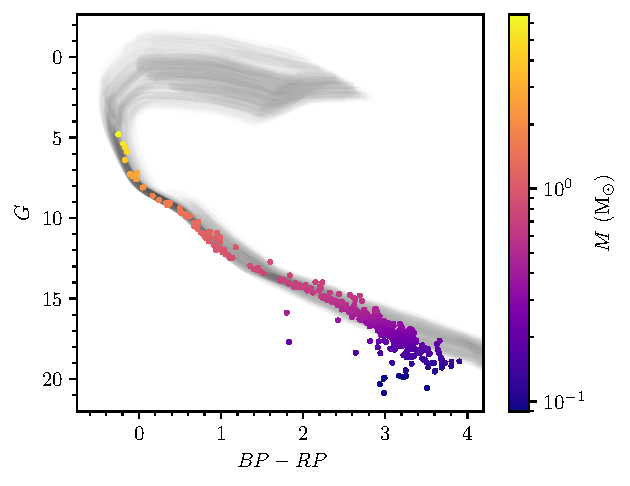
\includegraphics[width=0.8\textwidth]{fig/c4/masses_stellar.pdf}
    \caption[CMD of NGC~2451A with stars shaded by their median sampled stellar mass]{CMD of NGC~2451A with stars shaded by their median sampled stellar mass from interpolation against cluster isochrones. 100 isochrones sampled from the age-determination neural network in Paper 2 are plotted in black.}
    \label{fig:dynamics:masses:stellar_masses}
 \end{figure}

 The first step in deriving the photometric mass of a cluster requires calculating the masses of the cluster's member stars. To do so, I follow a similar method to those as used in numerous other works, such as \cite{meingast_extended_2021} and \cite{cordoni_photometric_2023}.

Using isochrone fits from Paper 2 and assuming solar metallicity for all clusters, PARSEC isochrones \citep{bressan_parsec_2012} were interpolated to predict mass as a function of G-band magnitude, $m(G)$. In general, this is sufficient for most member stars within clusters, and derives the most accurate stellar mass given \gaia\ G-band photometry and other calculated cluster parameters. 
 
However, particularly for older clusters, many clusters have giant stars beyond the turn-off point that dip below the tip of the main sequence (see Fig.~\ref{fig:intro:history:isochrones}), meaning that a single value of $G$ can correspond to multiple different stellar masses $m$. Hence, for isochrones where the a direct conversion from magnitude to stellar mass is not possible for all stars, the interpolation region was split into a main sequence and turn-off point component. For stars near to and above the turn-off point, $BP-RP$ colours were also used to select the best fitting stellar mass. I do not use colours across the entire isochrone as \gaia\ DR3 colours can be under-estimated for stars fainter than $G\sim19$ \citep[especially in the BP band,][]{riello_gaia_2021}, and it is hence likely to be more accurate to limit the use of colour information in stellar mass interpolation as much as possible.

Since the age inference neural network from Paper 2 used variational inference to incorporate uncertainties, it can be sampled to produce multiple estimates on parameters for each cluster. Hence, for every cluster, the stellar mass interpolation process was repeated 100 times, allowing the uncertainty inherent from age and extinction determination to be incorproated into the stellar masses stoachastically. Figure~\ref{fig:dynamics:masses:stellar_masses} shows the CMD of NGC~2451A, with its member stars shaded by their median sampled stellar mass and the 100 isochrone samples plotted in the background.

As this interpolation process does not account for binaries, these stellar masses can be considered as being roughly equal to the stellar mass of the primary stars of any binary system. A separate correction for binaries is discussed and added later in Sect.~\ref{sec:dynamics:masses:binaries}.


\subsection{Correction for selection effects}
\label{sec:dynamics:masses:selection}

\begin{figure}[p]
    \centering
    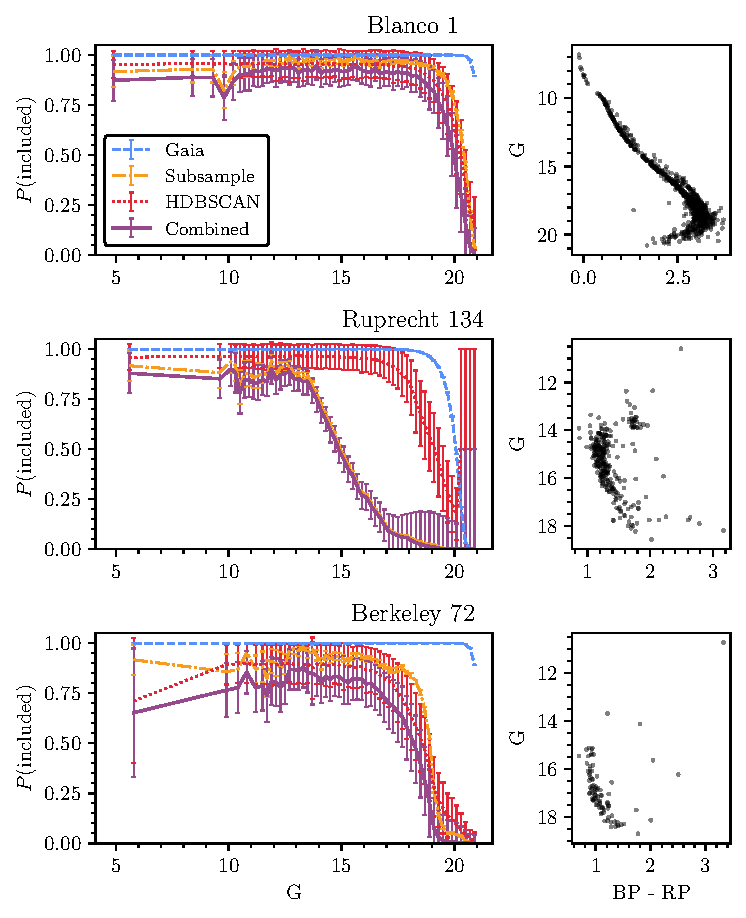
\includegraphics[width=\textwidth]{fig/c4/mass_selection_functions.pdf}
    \caption[Estimated cluster selection functions for three OCs from Paper~2: Blanco~1, Ruprecht~134, and Berkeley~72]{Estimated cluster selection functions for three OCs from Paper~2: Blanco~1, Ruprecht~134, and Berkeley~72. The left column shows computed cluster selection functions and a combined cluster selection function after accounting for all three dominant selection effects. The right column shows the CMD of each considered cluster for comparison.}
    \label{fig:dynamics:masses:selection_effects}
\end{figure}

Next, it is important to correct for selection effects. In Paper 2, we derived cluster membership lists down to magnitudes as faint as $G\sim20$. However, particularly at the faint end, clusters still become increasingly incomplete. This depends strongly on the position of the cluster in the disk: in the most extreme cases, for clusters in regions with high numbers of sources (such as towards the galactic centre), incompleteness is clear from magnitudes as bright as $G=17$. It is clear that accurate determination of cluster masses will require incorporation of these effects. The selection function of \gaia\ and subsamples of it have been relatively well studied in works such as \cite{boubert_completeness_2020,boubert_completeness_2020-1}, \cite{boubert_completeness_2020-1}, \cite{rix_selection_functions_2021}, \cite{cantat-gaudin_empirical_model_2023}, and \cite{castro-ginard_estimating_selection_2023}, whose work I will adapt in this section to calculate star cluster selection functions.

The incompleteness of a cluster's membership list in Paper 2 is governed by three primary effects. Firstly, there is the simple probability that a source with attributes $\vec{q}=\left\{ l,b,G,... \right\}$ appears in the \gaia\ catalogue at all, $S_C^\text{parent}(\vec{q})$. To compute this, I use the selection function presented in \cite{cantat-gaudin_empirical_model_2023}, who compared the \gaia\ catalogue with deep photometric surveys of the galactic disk and globular clusters, deriving $S_C^\text{parent}(\vec{q})$ empirically as a function of the position and magnitude of a source for the entire \gaia\ DR3 catalogue. This builds on the purely theoretical \gaia\ selection function derived in \cite{boubert_completeness_2020,boubert_completeness_2020-1}. 

However, many of the sources in \gaia\ do not include proper motions and parallaxes, do not include full photometry, or do not have reliable astrometry. Our Paper 2 membership lists were computed for a subsample of \gaia\ sources: namely, those with five or six parameter astrometric solutions, $G$, $BP$, and $RP$ photometry, and a \cite{rybizki_classifier_2022} v1 quality flag greater than 0.5, indicating that the source is likely to have reliable astrometry. This constitutes a subsample of 729~million stars from the overall \gaia\ DR3 catalogue.

To compute the probability that a source appears in this subsample given that it is also in the \gaia\ catalogue, i.e. $S_C^\text{subsample}(\vec{q} \mid \vec{q}\text{ in parent})$, I use the method outlined in \cite{castro-ginard_estimating_selection_2023} and based on \cite{rix_selection_functions_2021}. Firstly, sources are binned based on their attributes $\vec{q}$. Then, within bins, the chance that a source with attributes $\vec{q}$ appears in the subsample is modelled as a binomial distribution $\mathcal{B}(n,\,p)$, where $n$ is the number of sources in the \gaia\ catalogue in this bin with attributes $\vec{q}$ and $p$ is the probability that a source with these attributes makes it into the subsample of valid stars. In practice, $p$ is unknown; hence, an uninformative uniform Beta distribution prior on $p$ given the number of observed sources in the bin is used \citep[see ][for full methodology]{castro-ginard_estimating_selection_2023}.

In practice, one must choose the attributes $\vec{q'}$ on which the selection function is assumed to depend. The subsample of stars we use is almost entirely dependent on astrometric quality. The astrometric quality of \gaia\ is strongly correlated with sky position and G-band magnitude, corresponding to background star density, the number of scans of a given position by the \gaia\ telescope, and the brightness (signal to noise ratio) of a source \citep{lindegren_gaia_2021}. Hence, I compute $S_C^\text{subsample}(\vec{q} \mid \vec{q}\text{ in parent})$ as a function of position and magnitude, selecting a region corresponding roughly to the on-sky extent of a cluster for consideration and binning them in bins of size $0.2$~mag. Bins were expanded until every bin contained at least ten sources, ensuring that no range of the selection function was under-sampled, but while preserving high resolution between $11 < G < 20$ where most sources in \gaia\ are.

Finally, I also found that the selection function of star cluster membership lists could depend on effects due to our adopted clustering algorithm and methodology in Paper~2, which is the probability that a given source is assigned as a member of a cluster by our clustering algorithm given that it appears in the subsample of valid sources considered for clustering analysis, $S_C^\text{algorithm}(\vec{q} \mid \vec{q}\text{ in subsample})$. Especially at high distances or within crowded fields, cluster proper motions and parallaxes become relatively uninformative, with many cluster members becoming relatively indistinguishable from field stars in these axes of \gaia\ astrometry. For distant clusters such as King~9, which is at a distance of $\sim6$~kpc, this can have a strong effect on our membership lists. Our adopted clustering algorithm from Paper 2, HDBSCAN, is density-based -- meaning that members are only assigned to a given cluster if they increase the contrast of a given cluster against unclustered stars. In practice, this means that stars away from the mean cluster proper motion or parallax are less likely to be assigned as cluster members, with many probably being missed. This is particularly dominant for faint sources at which \gaia\ astrometric errors can be on the order of (or even larger than) our measured cluster proper motion and parallax dispersions, meaning that many member stars are likely missed for the most distant objects. Errors on positions are correspondingly negligible compared to the generally no smaller than $0.1^\circ$ size of clusters, and so this effect is only of concern for cluster proper motions and parallaxes.

To model this effect, I developed a novel stochastic technique to simulate the probability that a source would have mean \gaia\ astrometry within the detected HDBSCAN cluster. Firstly, the cluster detected by HDBSCAN is modelled as a three-dimensional ellipsoid in proper motion and parallax space. Then, 100\,000 stars with magnitudes uniformly distributed in the range $2 < G < 21$ were simulated, with astrometric errors assigned to each star depending on the error distribution of sources in the on-sky vicinity of a cluster. For each star, ten mean astrometric positions were simulated, given its simulated \gaia\ astrometric errors which form a multivariate normal distribution in proper motion and parallax space. For each simulation, a mean astrometric position within the cluster ellipsoid is assumed to be assigned as a cluster member, and a star whose mean astrometric position is outside of the cluster ellipsoid is assumed to be assigned as a non-member. The results of these simulations for each cluster are binned using the same bins as the subsample selection function, and are then combined into an estimated per-cluster clustering algorithm selection function as a function of G-band magnitude. Poisson uncertainties are computed as the uncertainties on these bins.

Finally, all three independent selection effects are multiplied together, giving the total cluster selection function $S_C^\text{cluster}$:

\begin{equation}
    S_C^\text{cluster} = 
    S_C^\text{parent}(\vec{q})
    \cdot
    S_C^\text{subsample}(\vec{q} \mid \vec{q}\text{ in parent})
    \cdot
    S_C^\text{algorithm}(\vec{q} \mid \vec{q}\text{ in subsample}).
    \label{eqn:dynamics:masses:selection_function}
\end{equation}

Figure~\ref{fig:dynamics:masses:selection_effects} shows the computed cluster selection functions for three OCs: Blanco~1, Ruprecht~134, and Berkeley~72. Blanco~1 is a nearby ($d\approx240$~pc), high galactic latitude OC that suffers minimally from background crowding and is easy to separate from field stars. Its selection function is mostly complete down to $G\sim19$. On the other hand, Ruprecht~134 is an older, more distant cluster ($d\approx2.3$~kpc) that is in one of the densest regions of the galactic disk, with $l=0.3^\circ$ and $b=-1.6^\circ$. It is probably one of the most incomplete clusters in our entire catalogue. Its incompleteness is mostly due to the subsample selection function, as many sources do not have high enough quality \gaia\ astrometry to be included in our subsample of considered sources. Finally, Berkeley~72 is a distant, smaller cluster ($d\approx5.1$~kpc) whose members are more difficult to separate from field stars. Like many distant objects, the selection function of Berkeley~72 appears mostly dominated by the selection function of our clustering algorithm from Paper~2 when applied with our methodology. 

It is also worth noting that in general, no clusters appear to have a range in $G$ in which their CMD is 100\% complete. Many of these missing stars across all magnitudes are likely to be binaries. Other than for a small subsample of around 1~million sources, \gaia\ DR3 astrometric fits assume that each source is a single star. Hence, binaries with deviations large enough to be detectable by \gaia\ can have poor-quality astrometric fits, resulting in high reduced $\chi^2$ values and high error astrometry that is rejected by quality cuts such as the one used for our subsample of stars \citep[][; see also Sect.~\ref{sec:intro:history:gaia:background}]{lindegren_gaia_2021}.



\subsection{Correction for unresolved binaries}
\label{sec:dynamics:masses:binaries}

Given that the stellar mass inference in Sect.~\ref{sec:dynamics:masses:selection} only calculated the masses of stellar primaries, assuming in the process that every star is single, it is important to also correct for an additional increase to cluster mass functions due to unresolved binaries.

Recently, measurements of the binary star fraction in a number of clusters have been made using \gaia\ DR3 photometry, with \cite{cordoni_photometric_binaries_2023} measuring this for 78 reliable OCs and \cite{donada_multiplicity_fraction_2023} measuring this for 202 OCs within 1.5~kpc. Both works are only able to measure the binary star fraction down to mass ratios of $q\approx0.6$, noting that it becomes difficult to disentangle lower mass ratio binaries from the main sequence of single stars, particularly for clusters with differential extinction. Given that the mass ratio distribution of binaries in the field has been shown to peak around $q\sim0.3$ \citep{moe_mind_2017}, it is hence unlikely to be possible using \gaia\ DR3 photometry alone to accurately measure the full mass ratio distribution of unresolved and resolved binary stars within a cluster, let alone across a large sample of clusters such as the 7167 in our catalogue from Paper 2.

For now, I use the selection effect corrected relations for multiplicity fraction, companion star frequency, and mass ratio of field stars from \cite{moe_mind_2017} to apply binary star corrections to each cluster mass bin. In addition, to calculate the fraction of unresolved to resolved binary stars, simulations of clusters and the astrometry of binary stars assuming the period and eccentricity distributions from \cite{moe_mind_2017} were conducted using \texttt{SPISEA} \citep{hosek_jr_pypopstar_2020} and \texttt{astromet} \citep{penoyre_astrometric_2022,penoyre_astrometric_2022-1}, with a binary correction being applied proportional to however many resolved or unresolved binaries were expected for each cluster.

Incorporation of these binary star corrections results in cluster mass bins that are inflated by around 10\% to 30\%, depending on the distance of the cluster and how many of its stars are likely to be in unresolved or resolved binaries. Uncertainties around binary star fraction likely add an upto 30\% additional uncertainty on my derived cluster masses, since a single relation is applied to all clusters. 

Before the final publication of this chapter in a paper, it may be possible to improve this binary star correction further. However, this simple correction may already be sufficient, since determination of the binary star fraction across all mass ratios for all (or even $\sim5$\%) of the 7167 clusters is not feasible with current available data.


\subsection{Mass function fits}
\label{sec:dynamics:masses:imf_fits}

\begin{figure}[p]
    \centering
    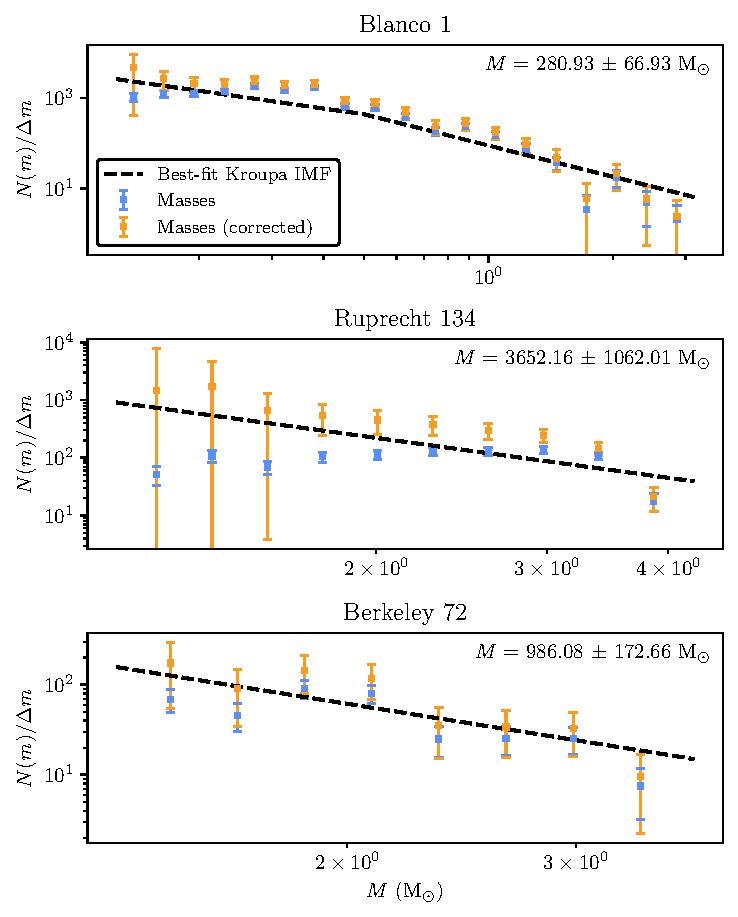
\includegraphics[width=\textwidth]{fig/c4/mass_functions.pdf}
    \caption[Mass function fits to the three OCs from Fig.~\ref{fig:dynamics:masses:selection_effects}]{Mass function fits to the three OCs from Fig.~\ref{fig:dynamics:masses:selection_effects}. The blue points show measured binned stellar masses, the orange points show these masses after correcting for selection effects and modest assumptions about binary stars, and the black dashed line shows the best-fitting Kroupa IMF. The integral of the cluster mass function is written in the top right of each plot.}
    \label{fig:dynamics:masses:mass_functions}
\end{figure}

Having calculated accurate completeness and binary-corrected mass bins for every cluster, I next used these mass measurements to calculate the total mass of every cluster. To do so, I fit a \cite{kroupa_variation_2001} initial mass function (hereafter Kroupa IMF) to the mass function of each cluster using least squares fitting. The integral of the Kroupa IMF from 0.03~\MSun to the highest observed stellar mass in the cluster is then taken as the mass value for the cluster.

One could also fit bespoke mass functions to each cluster \citep[e.g. as in][]{cordoni_photometric_binaries_2023}. The IMF is known to be a broken power law for most populations, with a break point around 0.5~\MSun \citep{kroupa_variation_2001}. However, low masses are poorly resolved for many of the clusters in our sample, with clusters more distant than $\sim1$~kpc or clusters with reddening values $A_V \gtrsim 2$ having few or no stars at masses lower than 0.5~\MSun. Hence, it would not be possible to fit a two-part mass function to these clusters, preventing an accurate estimate of their true total mass. The `safer' option in this case is to fit Kroupa IMFs to all clusters, deriving masses on the same scale with the same assumed mass function.

Some N-body simulations have suggested that cluster mass functions become depleted of low mass stars over time, due to lower mass stars being preferentially ejected from clusters \citeme{this}. Before publishing this work, it may also be insightful to fit bespoke mass functions to nearby clusters to investigate this effect. However, this would likely also require a better determination of a binary star mass function correction for each cluster, which may be beyond the scope of this work.

Figure~\ref{fig:dynamics:masses:mass_functions} shows mass function fits to the three clusters from Fig.~\ref{fig:dynamics:masses:selection_effects}. Generally, Kroupa IMFs are a reasonable approximation for most clusters, and the integral of these mass functions produces reasonable values of the total mass for each cluster. 

More work should be done to improve the fitting process of cluster mass functions before publication. One can see in Fig.~\ref{fig:dynamics:masses:mass_functions} that outlier points can over-constrain fits and result in erroneously higher or lower masses (such as the highest mass bin for Ruprecht~134, or some of the higher mass bins for Blanco~1 -- in both cases, these reduce the final total cluster mass by a large amount). I intend to upgrade the least squared fitting of cluster mass functions to use a more statistical approach that includes rejection of outlier points, which should improve the overall accuracy of derived cluster masses.


\subsection{Jacobi radius inference}
\label{sec:dynamics:masses:jacobi}

\begin{figure}[t]
    \centering
    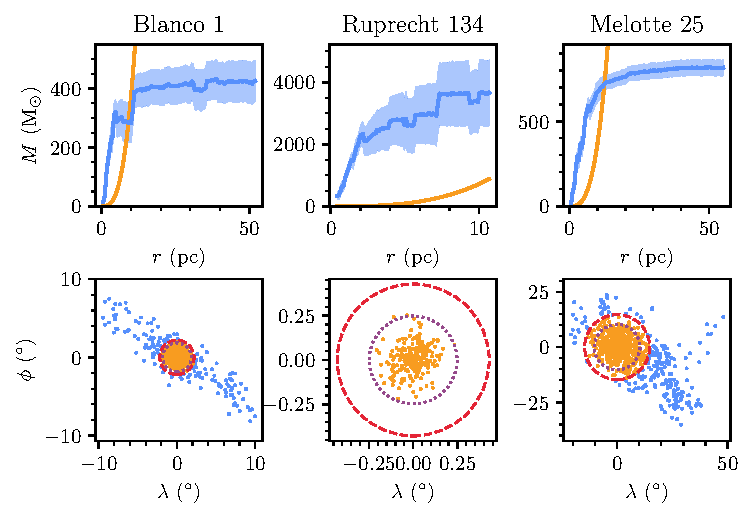
\includegraphics[width=\textwidth]{fig/c4/masses_jacobi_radii.pdf}
    \caption[Jacobi radius determination for three OCs: Blanco~1, Ruprecht~134, and Melotte~25]{Jacobi radius determination for three OCs: Blanco~1, Ruprecht~134, and Melotte~25 (the Hyades). Each of the three columns corresponds to each cluster. \emph{Top row:} the estimated total mass contained within a radius $r$ is shown in blue ($M_\text{obs}(r)$), with the $1\sigma$ error region shaded on the plot. The orange line shows the theoretical amount of mass contained within a radius $r$ according to the Jacobi radius equation ($M_J(r)$, Eqn.~\ref{eqn:intro:jacobi_radius}). The intersection of these two lines corresponds to the cluster's $r_J$. \emph{Bottom row:} the distribution of cluster member stars. To remove spherical distortions, positions are rotated to an arbitrary coordinate frame with longitude $\lambda$ and latitude $\phi$ centred on the cluster centre. Stars within $r_J$ are shown in orange while stars outside of $r_J$ are shown in blue. The dashed red line shows $r_J$, while the dashed purple line corresponds to the approximate value of $r_t$ determined in Paper 2.}
    \label{fig:dynamics:masses:radii_examples}
\end{figure}

\begin{figure}[t]
    \centering
    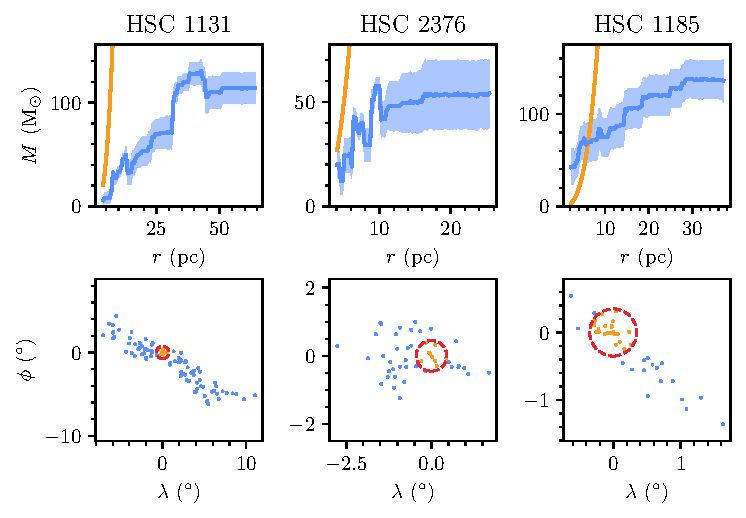
\includegraphics[width=\textwidth]{fig/c4/masses_jacobi_determination.pdf}
    \caption[Jacobi radius determination for three candidate new OCs from Paper 2 that were highlighted as example new objects]{Jacobi radius determination for three candidate new OCs from Paper 2 that were highlighted as example new objects (see Sect.~\ref{c3:sec:discussion-moving_groups} and Fig.~\ref{c3:fig:sus_clusters}). The plot is formatted the same as Fig.~\ref{fig:dynamics:masses:radii_examples}. The most likely Jacobi radius for HSC~1131 and HSC~2376 is shown, although $M_\text{obs}(r)<M_J(r)$ for all radii for both clusters and they are hence more likely to be MGs (see text).}
    \label{fig:dynamics:masses:radii_examples_sus}
\end{figure}

Finally, having constructed a pipeline to calculate cluster masses, I used these methods to infer the Jacobi radius $r_J$ of the clusters in our sample. Recalling Sect.~\ref{sec:intro:theory:profile}, the Jacobi radius defines the radius within which a star cluster's gravitational potential is greater than the potential of the Milky Way. Within this radius, all stars have the potential to be bound together. I define the amount of mass within this radius as the Jacobi (or bound) mass $M_J$ of each cluster.

The Jacobi radius of each cluster was calculated using the method of \cite{meingast_extended_2021}. Firstly, I calculated the circular and epicyclic frequencies at the cluster's distance from the galactic centre using \texttt{galpy} \citep{bovy_galpy_python_2015} and the \texttt{MWPotential2014} potential model defined in \cite{bovy_galpy_python_2015}. Next, for each cluster, the theoretical value of the Jacobi mass as a function of radius $M_J(r)$ was calculated at all radii outwards from the centre of the cluster. Finally, the observed cluster mass as a function of radius $M_\text{obs}(r)$ was calculated by repeating the process of binning stars by mass, applying a correction for unresolved binaries, and fitting Kroupa IMFs to the resulting cluster mass functions. The radius at which $M_\text{obs}(r) = M_J(r)$ is then hence the Jacobi radius of the cluster. Only radii at which the cluster would have at least ten observed bound members were considered, differentiating any potential bound cluster from multiple star systems and in accordance with common minimum limits on the size of an OC \citep{cantat-gaudin_clusters_2020,portegies_zwart_young_2010}.

There are two special cases of this method worth discussing. Firstly, for clusters without a valid Jacobi radius, $M_\text{obs}(r)<M_J(r)$ at all radii. These clusters can be considered to have no radius at which their potential is stronger than that of the Milky Way, and would be better classified as MGs instead of OCs. For these clusters, I take the radius at which they are closest to having a valid Jacobi radius and compute the probability of a cluster nevertheless having a valid Jacobi radius, given the uncertainties on their computed observed mass. For most clusters with $M_\text{obs}(r)<M_J(r)$ for all $r$, this probability is near zero; although some edge-case objects may still have a small chance of having a valid Jacobi radius. Secondly, some clusters have an observed mass greater than their Jacobi mass even at the highest angular distance of any member star from the cluster core. This is particularly common for more distant or difficult to detect clusters, and is likely becuase they do not have detected member stars out to their true $r_J$. For these clusters, I compute $r_J$ for the mass of the entire detected cluster, giving a Jacobi radius larger than the total extent of the cluster on the sky. This value is likely to be an under-estimate of the true cluster $r_J$ as the undetected outskirts of the cluster would increase $r_J$ further.

Figure~\ref{fig:dynamics:masses:radii_examples} shows $M_\text{obs}(r)$ and $M_J(r)$ for three clusters: Blanco~1, Ruprecht~134, and Melotte~25 (the Hyades), in addition to the member stars within these radii. Firstly, it can be noted that at $r<r_J$, $M_\text{obs}(r)$ is greater than $M_J(r)$ for Blanco~1 and Melotte~25, showing that these are reliable clusters with a range of radii where enough mass is present that the cluster's gravitational potential is stronger than that of the Milky Way. Ruprecht~134 is a more distant and difficult to detect cluster for which $M_\text{obs}(r)$ is always greater than $M_J(r)$. The Jacobi radius of its total population is larger than the observed maximum radius of the cluster.

This method also appears to be a good test of whether an object is an OC or an MG. Figure~\ref{fig:dynamics:masses:radii_examples_sus} shows the Jacobi radius determination for three candidate OCs from Paper~2 that were highlighted as example new objects. In Sect.~\ref{c3:sec:discussion-moving_groups}, we suggested that HSC~1131 and HSC~2376 were sparse objects that appear more compatible with moving groups, and HSC~1185 is an object with a denser core that could be compatible with a small OC. Figure~\ref{fig:dynamics:masses:radii_examples_sus} suggests that this is the case: HSC~1131 and HSC~2376 both do not have a valid Jacobi radius, while HSC~1185 is compatible with a small cluster with around 65~\MSun of bound stellar content.

Finally, it is worth commenting on a remaining issue with this calculation that I hope to fix before publication. $M_\text{obs}(r)$ values in Figs.~\ref{fig:dynamics:masses:radii_examples}~and~\ref{fig:dynamics:masses:radii_examples_sus} often jump up and down. In addition, the fitted mass within a radius $r$ can even decrease as $r$ increases, as appears to be the case for Blanco~1. This is due to issues with mass function fitting identified in Sect.~\ref{sec:dynamics:masses:imf_fits}, which causes mass function fits to be unstable and biased by outlier mass bins. Improvements to mass function fitting should make this process more stable and should improve the accuracy of $r_J$ determination for all clusters.



% -------------------------------------
\section{Velocity dispersion inference}
\label{sec:dynamics:velocities}

While the derived cluster masses and Jacobi radii from the previous section are effective to determine which clusters have the possibility of being bound, the dynamical state of a cluster depends not only on its mass and radius, but also its velocity dispersion (Eqn.~\ref{eqn:intro:virial_ratio}). Velocity dispersions from \gaia\ data have been used in a number of works such as \cite{bravi_gaia-eso_2018}, \cite{kuhn_kinematics_2019}, and \cite{pang_3d_2021} to probe the current dynamical status of star clusters. Even for clusters with a valid Jacobi radius, it may be that their velocity dispersion is so high that it is clear the cluster is a dense (but unbound) object. 

While some dynamical studies have used radial velocities to study the dynamics of OCs \citep[e.g.][]{bravi_gaia-eso_2018} or proper motions in combination with radial velocities \citep[e.g.][]{evans_mass_2022-1}, I aim to use exclusively proper motions \citep[e.g. as in][]{kuhn_kinematics_2019}, as they are the only measurement available reliably across the entire sample of clusters. Hence, in this section, I outline a method to derive approximate cluster velocity dispersions from cluster proper motions based on a simple Gaussian model.


\subsection{Gaussian velocity dispersion model}
\label{sec:dynamics:velocities:model}

\begin{figure}[t]
    \centering
    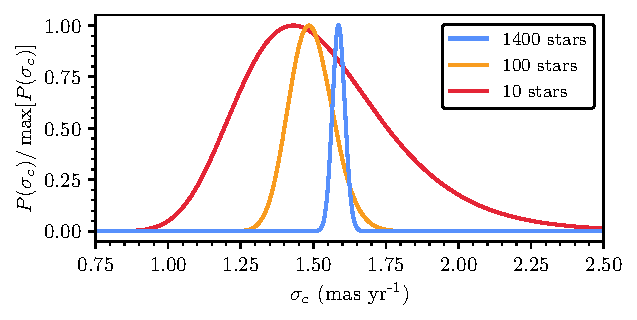
\includegraphics[width=\textwidth]{fig/c4/dispersion_pdf.pdf}
    \caption[Proper motion dispersion likelihood in Eqn.~\ref{eqn:dynamics:velocities:likelihood} evaluated for different subsets of stars in Melotte~22]{Proper motion dispersion likelihood in Eqn.~\ref{eqn:dynamics:velocities:likelihood} evaluated for different subsets of stars in Melotte~22 (the Pleiades). The blue curve shows all 1400 stars within my calculated value of $r_J$. The orange and red curves are for sets of 100 and 10 stars respectively that were randomly sampled from the overall cluster, showing how the likelihood becomes broader and assymmetric as uncertainty on the true value increases.}
    \label{fig:dynamics:velocities:pdfs}
\end{figure}

By definition, dynamically relaxed virialised clusters are expected to have an isothermal (Maxwellian) velocity dispersion that will be well described by a Gaussian \citep{king_structure_1966,portegies_zwart_young_2010}, assuming that stars within a cluster of $n$ stars have independent, uncorrelated velocities -- namely, that there is no overall axis of rotation within the cluster, and the cluster is well described by a \cite{king_structure_1966} profile. Hence, the assumption of a Gaussian model for the distribution of cluster proper motions is likely to be a good approximation for most OCs, and I approximate cluster velocity dispersions as a symmetrical multivariate Gaussian distribution with a single dispersion in all axes, $\sigma_c$.

Given the set of all proper motion measurements for stars within a cluster $\{\vec{\mu}\}$, which each have corresponding covariances from the set of all covariance matrices  $\{\Sigma\}$, and a mean cluster proper motion $\vec{\mu}_c = (\mu_{\alpha, c}, \mu_{\delta, c})$, the likelihood of the observed data given these cluster parameters is hence given by

\begin{equation}\label{eqn:dynamics:velocities:likelihood}
    \mathcal{L} 
    = P(\{\vec{\mu}\}\mid\vec{\mu}_c,\sigma_c,\{\Sigma\}).
\end{equation}

Every $i^{th}$ star in the cluster has a true proper motion $\vec{\bar{\mu}}_i~=~(\bar{\mu}_{\alpha,~i},\bar{\mu}_{\delta,~i})$, which is drawn from the two-dimensional Gaussian

\begin{equation}\label{eqn:dynamics:velocities:generative_model}
    P(\vec{\bar{\mu}}_i \mid
    \vec{\mu}_c, \sigma_c)_i \sim \mathcal{N}(\vec{\mu}_c \mid \sigma_c),
\end{equation}

\noindent
where $\mathcal{N}$ denotes a bivariate normal distribution.

However, \emph{Gaia} proper motion measurements have uncertainties, and the measured proper motion of every source $\vec{\mu}_i~=~(\mu_{\alpha,~i},~\mu_{\delta,~i})$ is the true proper motion $\vec{\bar{\mu}}_i$ convolved with Gaussian measurement uncertainties. $\vec{\mu}_i$ has a covariance matrix $\Sigma_i$ defined as:

\begin{equation}
    \Sigma_i = 
        \begin{bmatrix}
        \sigma_{\mu_\alpha, i}^2 
        & \rho_i \sigma_{\mu_\alpha, i} \sigma_{\mu_\delta, i}\\
        \rho_i \sigma_{\mu_\alpha, i} \sigma_{\mu_\delta, i}
        & \sigma_{\mu_\delta, i}^2
        \end{bmatrix}
\end{equation}

\noindent
where $\sigma_{\mu_\alpha, i}$ and $\sigma_{\mu_\delta, i}$ are the uncertainties on proper motions in right ascension and declination respectively, and $\rho_i$ is the covariance coefficient between them. Every measured proper motion $\vec{\mu}_i$ is therefore drawn from a bivariate normal distribution centred on the true proper motion of star $i$ $\vec{\bar{\mu}}_i$ as:

\begin{equation}\label{eqn:dynamics:velocities:measurement_model}
    P(\vec{\mu}_i \mid
    \vec{\bar{\mu}}_i, \Sigma_i)_i \sim \mathcal{N}(\vec{\bar{\mu}}_i \mid \Sigma_i),
\end{equation}

\noindent
which is the measurement model for each star which accounts for \emph{Gaia} astrometric uncertainties.

Since the true proper motion $\vec{\bar{\mu}}_i$ is unknown, all possible values of this parameter must be marginalised over to remove it from the likelihood and arrive at a final (solvable) equation. The final likelihood for each star is hence given by

\begin{equation}
    \mathcal{L}_i = P(\vec{\mu}_i \mid \vec{\mu}_c, \sigma_c, \Sigma)_i = 
    \int P(\vec{\mu}_i, \vec{\bar{\mu}}_i \mid \vec{\mu}_c, \sigma_c, \Sigma)_i \; d \vec{\bar{\mu}}_i.
\end{equation}

\noindent
Using the product rule and conditional independence between parameters, this can be expressed in terms of Eqns.~\ref{eqn:dynamics:velocities:generative_model}~and~\ref{eqn:dynamics:velocities:measurement_model} as:

\begin{equation}
    \mathcal{L}_i% = P(\vec{\mu}_i \mid \vec{\mu}_c, \sigma_c, \Sigma)_i
    = \int P(\vec{\mu}_i \mid \vec{\bar{\mu}}_i, \Sigma_i)_i \;
    P(\vec{\bar{\mu}}_i \mid \vec{\mu}_c, \sigma_c)_i \;
    d \vec{\bar{\mu}}_i.
\end{equation}

Finally, for all $n$ stars in the cluster, assuming that the set of all proper motion measurements $\{\vec{\mu}\}$ with corresponding covariances $\{\Sigma\}$ is independent, the final likelihood is given by:

\begin{equation}\label{eqn:dynamics:velocities:final_likelihood}
    \mathcal{L} 
    = P(\{\vec{\mu}\}\mid\vec{\mu}_c,\sigma_c,\{\Sigma\}) 
    = \prod_{i=1}^{n} \mathcal{L}_i.
\end{equation}

Evaluations of this likelihood for the Pleiades are shown in Fig.~\ref{fig:dynamics:velocities:binary_contamination}, as well as for smaller subsets of stars randomly sampled from the Pleiades. When the cluster dispersion is possible to measure precisely, the Eqn.~\ref{eqn:dynamics:velocities:likelihood} likelihood is symmetric; in less certain cases, the likelihood becomes assymetric, with a long tail towards high $\sigma_c$ values.

In practice, \emph{Gaia} measurements are not strictly independent, and coordinate frame distortions due to effects such as the radial motion of the cluster will cause clusters to have distorted, non-Gaussian proper motion distributions. In the next section, I discuss how cluster proper motions are corrected for various distortions arising from spherical geometry, cluster radial velocity projected into the tangential proper motion plane, and \gaia\ systematics.


\subsection{Coordinate frame and radial velocity corrections}
\label{sec:dynamics:velocities:correction}

Cluster proper motions are corrected in two ways. I remove the impact of an effect known as `perspective expansion' due to the relative motion of a cluster to the Sun. Particularly for clusters with high radial velocities such as the Hyades, this effect can cause stars to appear to expand or contract away from the centre of the cluster \citep{kuhn_kinematics_2019}. To first order, this contributes an excess proper motion $\Delta \mu_{\alpha^*,i}$ and $\Delta \mu_{\delta,i}$ to star $i$ given by \citep{vanleeuwen_parallaxes_proper_2009}:

\begin{equation}
    \Delta \mu_{\alpha^*,i} \approx \Delta\alpha_i \left( 
        \mu_{\delta,c} \sin\delta_c - \frac{v_{r,c} \varpi_c}{k}\cos\delta_c
    \right)
\end{equation}

\begin{equation}
    \Delta \mu_{\delta} \approx -\Delta\alpha_i \mu_{\alpha^*,c} \sin\delta_c - \Delta\delta_i \frac{v_{r,c}\varpi_c}{k},
\end{equation}

\noindent
where $\alpha_c$, $\delta_c$, $\mu_{\alpha^*,c}$, $\mu_{\delta,c}$, and $\varpi_c$ are the astrometric parameters for the cluster derived in Paper~2, $\Delta\alpha_i$ and $\Delta\delta_i$ are the distance in right ascension and declination of the star from the cluster centre, $v_{r,c}$ is the cluster radial velocity determined in Paper~2, and $k$ is a constant equal to 4.74. For 1418 clusters with no determined radial velocity (which are generally distant and would be minimally affected by perspective expansion), this correction was not applied.

In addition, to remove any possible spherical distortions on cluster proper motions, I rotate the coordinate frame of astrometric measurements and associated proper motions into a frame centred on the cluster centre determined in Paper~2. Errors on proper motions are transformed to the new frame. For most clusters, the effect of this correction is negligible; however, for clusters near to the poles of the adopted coordinate frame, this correction prevents cluster proper motions from having a ring-like distribution.

\subsection{Inference procedure}
\label{sec:dynamics:velocities:inference}

Finally, cluster velocity dispersions were inferred for all clusters with a maximum likelihood method. Only stars within the identified Jacobi radius of each cluster were considered when inferring $\sigma_c$, which mostly removes the signature of cluster tidal tails from clusters. In addition, only stars with a renormalised unit weight error (RUWE) value of less than 1.4 were considered, which should help to restrict inference to only stars with reliable astrometry and should remove some obvious astrometric binaries \citep{lindegren_gaia_2021,penoyre_astrometric_2022,penoyre_astrometric_2022-1}.

The full PDF and associated confidence intervals around the most likely $\sigma_c$ value were determined. To marginalise over and integrate the likelihood in Eqn.~\ref{eqn:dynamics:velocities:likelihood} quickly for all sources, a \texttt{C++} program was written using the integration package in the the GNU Scientific Library\footnote{\url{https://www.gnu.org/software/gsl/}}.


% -------------------------------------
\section{Results}
\label{sec:dynamics:results}


\subsection{Masses}
\label{sec:dynamics:results:masses}

\begin{figure}[t]
    \centering
    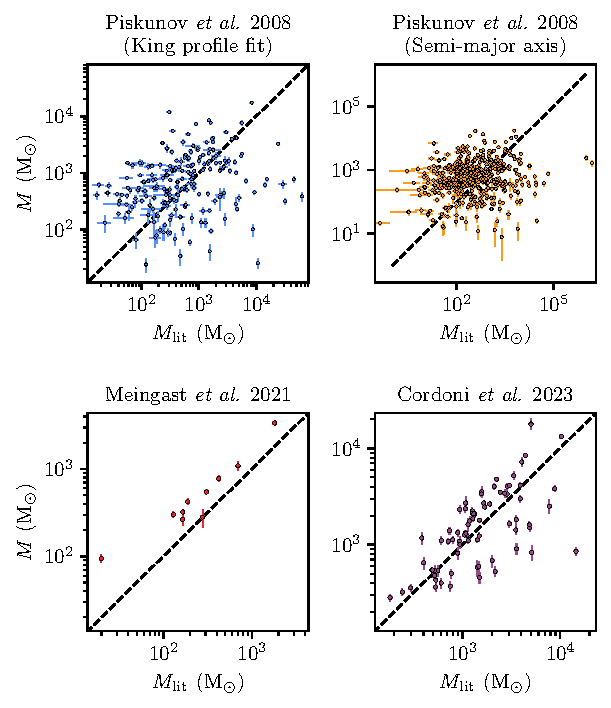
\includegraphics[width=\textwidth]{fig/c4/results_mass_comparison.pdf}
    \caption[TODO]{TODO}
    \label{fig:dynamics:results:mass_comparison}
\end{figure}


\subsection{Jacobi radii}
\label{sec:dynamics:results:radii}

\begin{figure}[t]
    \centering
    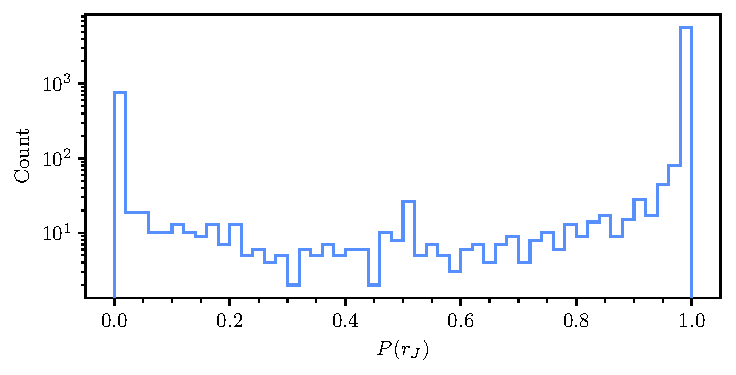
\includegraphics[width=\textwidth]{fig/c4/results_p_jac_distribution.pdf}
    \caption[TODO]{TODO}
    \label{fig:dynamics:results:jacobi_radii_distribution}
\end{figure}


\subsection{Virial ratios and binary star contamination}
\label{sec:dynamics:results:virial}

\begin{figure}[t]
    \centering
    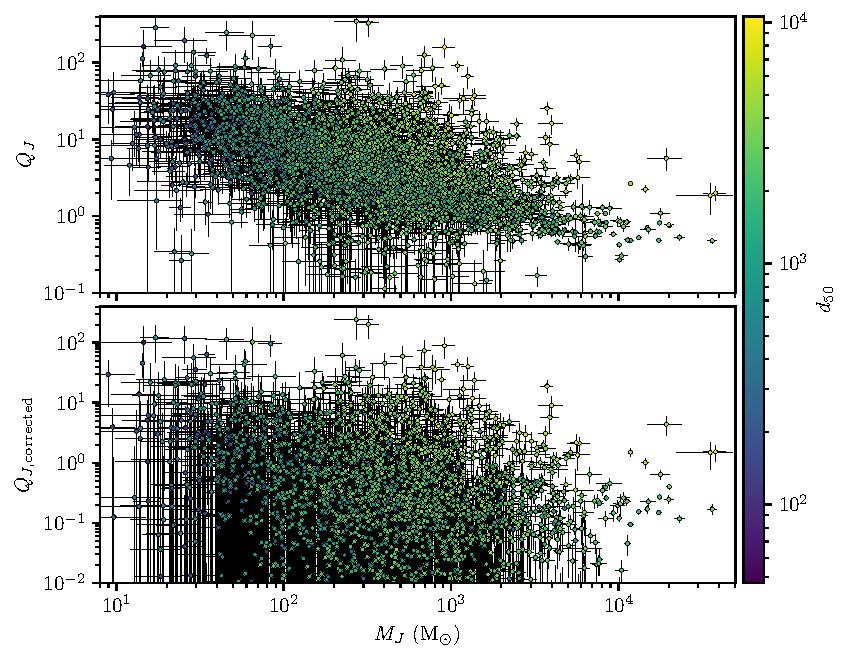
\includegraphics[width=\textwidth]{fig/c4/results_virial_vs_mass.pdf}
    \caption[TODO]{TODO}
    \label{fig:dynamics:results:virial_vs_mass}
 \end{figure}

 \begin{figure}[t]
    \centering
    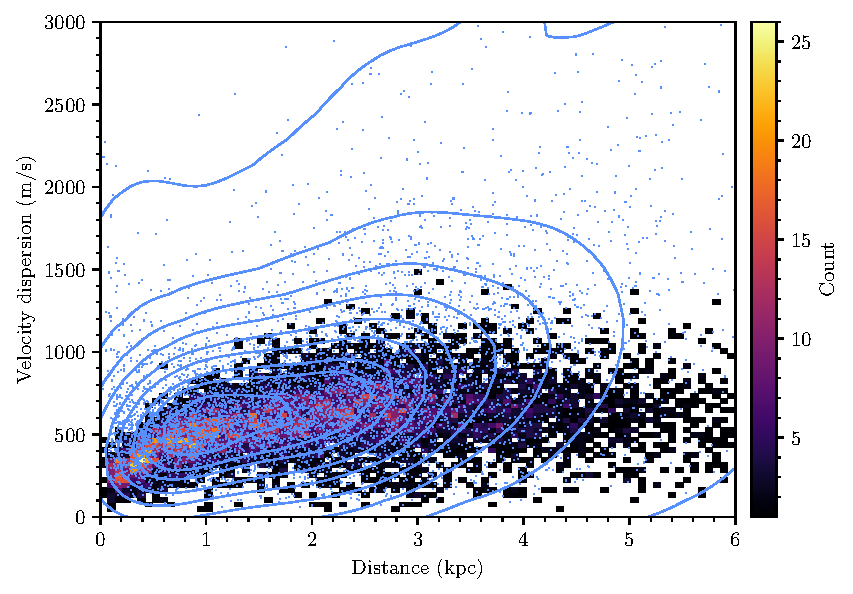
\includegraphics[width=\textwidth]{fig/c4/dispersion_binaries.pdf}
    \caption[TODO]{TODO}
    \label{fig:dynamics:velocities:binary_contamination}
\end{figure}

\begin{figure}[t]
    \centering
    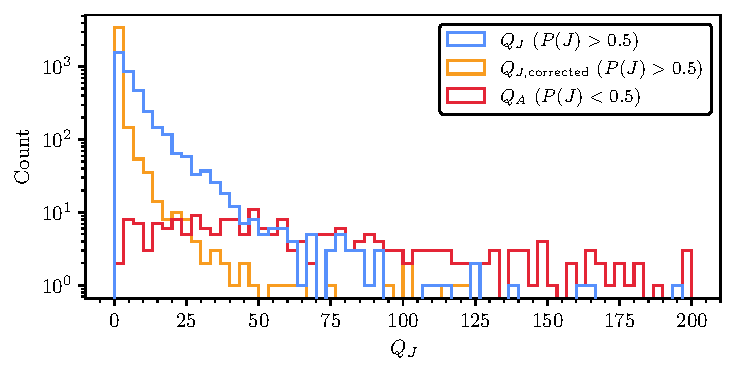
\includegraphics[width=\textwidth]{fig/c4/results_q_distribution.pdf}
    \caption[TODO]{TODO}
    \label{fig:dynamics:results:virial_ratio_distribution}
\end{figure}


\subsection{An updated observational definition of open clusters}
\label{sec:dynamics:results:definition}

\begin{table}[t]

% Define first header
\caption{\label{tab:dynamics:catalogue_results}TODO}

\centering
\begin{tabular}{lccc}
\hline\hline
Type & Criteria & Identifier & Count \\
\hline

OC & $P(r_J) > 0.5$ and $M_J < 50$ \MSun & & TODO \\
- bound OC & $Q_{J,\text{corrected}} \leq 10$ & \texttt{o} & TODO \\
- dissolving OC? & $Q_{J,\text{corrected}} \geq 10$ & \texttt{od} & TODO \\
- unbound OC? & $Q_{J,\text{corrected}} \geq 50$ & \texttt{ou} & TODO \\
\hline
MG & $P(r_J) > 0.5$ or $M_J < 50$ & & TODO \\
- without Jacobi component & $P(r_J) < 0.5$ & \texttt{m} & TODO \\
- with Jacobi component & $P(r_J) > 0.5$ & \texttt{mj} & TODO \\
\hline
GC & in \citeme{Vasiliev} & \texttt{g} & TODO \\
\hline
Too distant & $d >= 15$~kpc & & TODO \\
\hline

\end{tabular}

% \tablefoot{
% \tablefoottext{a}{}
% }

\end{table}    


% -------------------------------------
\section{Discussion}
\label{sec:dynamics:discussion}


\subsection{Completeness of the \gaia\ DR3 open cluster census}
\label{sec:dynamics:results:completeness}


% -------------------------------------
\section{Conclusions and areas for improvement before publication}
\label{sec:dynamics:conclusion}
     % INCLUDE: conclusion
% !TEX root = ../my-thesis.tex
%
\chapter{Conclusion}
\label{sec:conclusion}

\cleanchapterquote{No observational problem will not be solved by more data.}{Vera Rubin}{}


\section{Summary of the results of this work}

In this thesis, I worked to improve the methods for detecting, cataloguing, and analysing OCs using the astrometric and photometric data of \gaia -- targeting five broad problems with the current census of OCs. Beyond simply showing that these methodologies are effective, I used these methods to create the largest homogeneous catalogue of OCs to date. With a focus on rigorous, statistical approaches, I quantified the reliability of all objects in the catalogue and derived parameters for them, in addition to reporting over two thousand new star clusters and showing that over a thousand OCs reported before \gaia\ are unlikely to be real. Finally, I derived the largest ever sample of cluster masses and Jacobi radii, using them to distinguish between bound OCs and unbound MGs and derive an approximate completeness estimate for the \gaia\ DR3 OC census.

After reviewing the current status of the literature surrounding OCs in the introduction to this thesis, in the first scientific chapter (Sect.~\ref{sec:comparison}), I reviewed and trialled a number of different methods to recover OCs from \gaia\ data. Since the release of \gaia\ DR1, automated clustering algorithms have been used to tremendous success to detect new OCs in \gaia\ data or to derive membership lists for existing clusters \citep[e.g.][]{castro-ginard_new_2018,castro-ginard_hunting_2019,castro-ginard_hunting_2020,castro-ginard_hunting_2022,liu_catalog_2019,cantat-gaudin_characterising_2018,cantat-gaudin_clusters_2020,cantat-gaudin_gaia_2019,he_catalogue_2021,he_new_2022,hao_sixteen_2020,jaehnig_membership_2021}. However, despite the widespread use of numerous algorithms in dozens of different works, the different methodologies used in the literature had never been compared side by side for application on OCs.

In Sect.~\ref{sec:comparison}, I compared three different algorithms for OC recovery -- DBSCAN, HDBSCAN, and Gaussian mixture models. Using the results of a practical test of the three algorithms applied to \gaia\ DR2 data, I found that no algorithm was without flaws. However, HDBSCAN was clearly the most sensitive for OC recovery -- despite not having been used by any authors at the time for detecting OCs, with almost all works preferring to use DBSCAN or Gaussian mixture models. To mitigate issues with HDBSCAN reporting a high number of false positive clusters, I developed a computationally efficient statistical density test to postprocess standard OC clustering results and derive an astrometric S/N for candidate clusters, which acts as a description of the quality of detected objects. Finally, I was able to detect 41 new OCs within the data in this work. 

Having shown that HDBSCAN is the most sensitive method for OC recovery, in Sect.~\ref{sec:census}, I used \gaia\ DR3 data to conduct the largest all-sky blind search for OCs to date, searching for OCs amongst a total of 729~million stars. By conducting a single search with HDBSCAN, I was able to recover a large fraction of all reported OCs, including virtually all reliable objects from the previous largest catalogue of OCs of \cite{cantat-gaudin_clusters_2020}. To further classify objects by reliability, I used an approximately Bayesian neural network to classify clusters based on the compatibility of their CMD with a single population of stars. Simple modifications to this network architecture also allowed for the inference of ages, extinctions, and photometric distances to the clusters within the catalogue.

In total, the catalogue contains 7167 clusters, 2387 of which are candidate new objects. 4105 of these objects are of high quality, with 739 high-quality objects being new. This represents the largest homogeneous catalogue of OCs and OC candidates in the \gaia\ era. The catalogue was the first time that many recently reported OCs had been recovered by an independent work, allowing for the confirmation of over 2000 objects as being likely to be real. In addition, owing to the scope of the search, I was able to show that 1152 clusters from the pre-\gaia\ catalogue of \cite{kharchenko_global_2013} that are as yet undetected in \gaia\ data are unlikely to be real, representing the largest analysis to date of which clusters detected before \gaia\ are or are not real.

I showed that many of the clusters in the catalogue appear more compatible with unbound MGs, and that basic empirical cuts on mean cluster parameters are insufficient to remove MGs from the catalogue. Motivated by a need to differentiate between bound and unbound clusters more accurately, in Sect.~\ref{sec:dynamics}, I present preliminary results into a study to measure the masses, velocity dispersions, and Jacobi radii of the largest ever sample of clusters, with the aim to use these parameters to discern between OCs and MGs.

I derived these parameters for 6974 clusters, representing a catalogue of accurate cluster masses more than 70 times larger than the largest other catalogue of cluster masses using \gaia data. I showed that 82\% of the clusters from Sect.~\ref{sec:census} are compatible with bound objects, dropping to just 16\% of those within 250~pc where the Sect.~\ref{sec:census} catalogue appeared to be dominated by moving groups. I showed that cluster masses and Jacobi radii are an effective way to differentiate between MGs and OCs, refining the observational definition of OCs into a more theoretically grounded definition.

On the other hand, I found that velocity dispersions measured using proper motions are an unreliable way to probe the boundness of an OC or OC candidate. I conducted simulations that show that unresolved and resolved binary stars may dominate the velocity dispersion of most clusters, and especially those of lower masses. This is at odds with many recent results that have suggested that OCs are supervirial \citep[e.g.][]{bravi_gaia-eso_2018,kuhn_kinematics_2019,pang_3d_2021}, which typically do not correct for or address the possibility of binary star contamination of proper motion measurements.

In total, I was able to show that there are 5619 probable OCs in my catalogue, 3515 of which are of high quality. Using these samples of clusters, I derive the largest ever mass-dependent completeness estimate for the OC census, finding that the completeness is well-described by a log-linear relation until around 2700~pc, which appears to be the highest possible 100\% completeness limit for all masses of clusters in \gaia\ DR3.


\section{Outlook on the future of OC science}

At the beginning of this thesis, I painted a bright view of the scientific potential of OCs in the Milky Way. For over a century, these objects have played a key role in furthering our understanding of stellar and galactic evolution. Thanks to \gaia, Milky Way astronomy is currently undergoing a renaissance: but the methodologies and catalogues used to analyse OCs must keep pace with the incredible data that \gaia\ is providing. With this thesis, I have attempted to tackle the issues with the OC census I outlined in Sect.~\ref{sec:intro:aims:issues}; to conclude this thesis, I think it is interesting to discuss how I have tried to contribute to solving these problems, and how these problems could be further addressed in the future.

\subsubsection{Problem 1. The methods used to detect open clusters (and their biases)}


\subsubsection{Problem 2. The status of clusters discovered before \gaia}


\subsubsection{Problem 3. The status of clusters discovered with \gaia}


\subsubsection{Problem 4. The completeness of the open cluster census}


\subsubsection{Problem 5. The observational definition of open clusters}



By providing an overview of algorithms, I have contributed important analysis and information to the scientific literature, outlining the choices one could make in choosing an algorithm for OC recovery. Since its publication, my comparison of clustering algorithms has been cited by a number of works, with works such as \cite{dellacroce_ongoing_hierarchical_2023a} adopting HDBSCAN as well as the density test I designed for their analysis.

The census of star clusters from Sect.~\ref{sec:census} should remain useful to many in the literature for many years to come, particularly owing to the scope of the search and the sheer number of clusters catalogued accurately within one work. It has previously been claimed that it is not possible to construct such a large catalogue with only one algorithm \citep{cantat-gaudin_clusters_2020}. By proving this claim to not be true, my catalogue presents a new way to construct a census of OCs given any dataset. I hope that this will pave the way for future studies using \gaia\ DR4 and DR5 (as well as whatever is a successor to \gaia!), in which single homogeneous catalogues can be constructed with one algorithm.

Finally, given issues surrounding MGs in the census, the final chapter of this thesis (Sect.~\ref{sec:dynamics}) provides many results that will greatly improve the existing census as well as existing definitions of OCs. By deriving cluster masses and Jacobi radii for such a large sample, I show that a precise definition of OCs can be applied across the entire galactic disk. This work should be published as soon as possible, particularly given the role it will play in dramatically improving the usability of the results in the main catalogue of clusters.

With \gaia\ DR4 slated for release in around 2.5 years at the time of writing \citep[no sooner than the end of 2025,][]{gaia_collaboration_gaia_2022}, and \gaia\ DR5 coming around the end of the decade, there are multiple even larger data releases on the horizon. DR4 will provide proper motions with doubled accuracy, significantly more identified astrometric binary stars, and most likely improved processing that reduces the number of bad sources. An OC census constructed from a billion input sources should probably be a target to complete for DR4.

During the preparation of the catalogue in Sect.~\ref{sec:census}, I encountered many difficulties due to computational limitations. Chief amongst those was that the main loop of HDBSCAN is single threaded, greatly limiting how large of a dataset the algorithm can be run on, and meaning that the \gaia\ dataset had to be tiled into over 12\,000 separate regions that required a painstaking merging process to recombine. A faster, parallelised version of HDBSCAN is currently under development, and could offer a significantly more straightforward way to construct a blind search catalogue\footnote{\url{https://github.com/TutteInstitute/fast_hdbscan}}. In fact, given the pace of modern machine learning literature, I would not be surprised if an even better clustering algorithm for OC recovery emerges by the end of the decade -- particularly one that could utilise \gaia\ uncertainties effectively. Astronomers should continue to keep a close eye on the machine learning literature.

A question that I asked myself throughout my work on the catalogue of clusters was how much difference there really fundamentally is between different types of star cluster. The smallest, most heavily disrupted OCs (such as Platais~9) barely have a core, and are heavily reminiscent of MGs except for a small bound core of stars that will remain bound together for only a few million years. The fact that HDBSCAN detects so many MGs has been a problem that has taken my entire PhD to solve, culminating in Sect.~\ref{sec:dynamics} of this thesis. But it begs the question: is it even a bad thing to have MGs and OCs in the same catalogue? Given that dissolved OCs should be detectable as MGs for a few tens of Myr \citep{portegies_zwart_young_2010}, MGs are an important way to study the afterlife of OCs. On the other hand, stars can form in an unbound MG that stays together for a short duration (e.g. Monoceros~R2, Fig.~\ref{fig:intro:definition:comparison}); but at least in terms of age and chemical homogeneity, an MG that never derived from a bound cluster is more or less just as good as an OC to study stellar evolution (and is an important part of the stellar lifecycle regardless). Maybe \gaia's wealth of MGs are more of a blessing than a curse: these hundreds of objects probably deserve just as much study as OCs; and if the methods used to detect OCs can detect MGs at the same time, then why not do so?


\section{Final remarks}

Finally, as I reach the last sentences of this thesis, I want to emphasise just how important it is that work to improve the census of OCs does not end on this page of this thesis. New data, methodologies, theories, computational resources, and more will always be available. Since the times of the 1700s when the refracting telescope gained widespread use, the effort to improve the census of objects in the night sky has been never-ending. I expect that this long-held tradition will continue with future \gaia\ data releases as well as potential \gaia\ follow-ups such as \emph{GaiaNIR}. After all, in just five years since the release of \gaia\ DR2, the OC census has been changed beyond recognition by the incredible data available to modern Milky Way astronomers. I am excited to see where the open clusters take us next.




% SCIENCE REVIEW
% - step by step -> what did I do?
% - relate back to identified problems with the OC census

% HOW RELEVANT
% - how will people use my results?
% - how does it help others?

% TAKE HOME MESSAGE
% - gaia, lsst, gaianir is gonna keep on giving
% - improving the OC census will be a never-ending task, but the payoff is pretty gorgeous!



% --------------------------
% Back matter
% --------------------------
%
{%
\setstretch{1.1}
\renewcommand{\bibfont}{\normalfont\small}
\setlength{\biblabelsep}{0pt}
\setlength{\bibitemsep}{0.5\baselineskip plus 0.5\baselineskip}
\printbibliography[nottype=online]
\newrefcontext[labelprefix={@}]
\printbibliography[heading=subbibliography,title={Webpages},type=online]
}
\cleardoublepage

\phantomsection
\addcontentsline{toc}{chapter}{\listfigurename}
%\pdfbookmark[0]{List of Figures}{List of Figures}
\listoffigures
\cleardoublepage

\phantomsection
\addcontentsline{toc}{chapter}{\listtablename}
\listoftables
\cleardoublepage

% List of listings - doesn't seem to be necessary
% \phantomsection
% \addcontentsline{toc}{chapter}{List of Listings}
% \lstlistoflistings
% \cleardoublepage

\appendix\cleardoublepage
% !TEX root = ../my-thesis.tex
%
\chapter{Appendix}
\label{sec:appendix}



\section{Appendices for Chapter \ref{sec:comparison}}

\subsection{ADQL query used to download data}\label{app:c2:adql}

 \emph{Gaia}  DR2 data for this work was downloaded with the following ADQL query. \texttt{\{start\_number\}} should be replaced with the first possible \texttt{source\_id} of the desired pixel using Eqn.~\ref{c2:eqn:healpix}. \texttt{\{end\_number\}} should be replaced with the first possible \texttt{source\_id} of the next integer pixel.

\begin{verbatim}
SELECT
-- Gaia astrometry
g.source_id, g.l, g.b, 
g.ra, g.ra_error, g.dec, g.dec_error, 
g.parallax, g.parallax_error, 
g.parallax_over_error, 
g.pmra, g.pmra_error, g.pmdec, g.pmdec_error, 
g.astrometric_params_solved, 

-- Gaia photometry
g.phot_g_mean_mag, g.phot_g_mean_flux, 
g.phot_g_mean_flux_error, 
g.phot_bp_mean_mag, g.phot_bp_mean_flux, 
g.phot_bp_mean_flux_error, 
g.phot_rp_mean_mag, g.phot_rp_mean_flux, 
g.phot_rp_mean_flux_error, 
g.phot_bp_rp_excess_factor, 

-- Calculate HEALPix level 5 index
GAIA_HEALPIX_INDEX(5, g.source_id) 
  AS gaia_healpix_5, 
               
-- RUWE statistics
r.ruwe, 
               
-- CBJ+2018 distances
d.r_est, d.r_lo, d.r_hi, 
d.r_len, d.result_flag 
               
-- Inner join the tables
FROM gaiadr2.gaia_source AS g 
INNER JOIN 
  gaiadr2.ruwe 
  AS r 
  ON g.source_id = r.source_id 
INNER JOIN 
  external.gaiadr2_geometric_distance 
  AS d 
  ON g.source_id = d.source_id 
           
-- Select only valid points
WHERE g.source_id >= {start_number} 
AND g.source_id < {end_number} 
AND g.astrometric_params_solved=31 
AND g.phot_bp_mean_mag IS NOT NULL 
AND g.phot_rp_mean_mag IS NOT NULL
\end{verbatim}


%-------------------------------------------------------------------
\subsection{Comparison with other OC catalogues}\label{app:c2:comparison_with_cats}

We present brief comparisons with the results of other OC catalogues, in lieu of best practices proposed in \cite{cantat-gaudin_clusters_2020} and as a part of efforts towards generally improving the quality of the OC census, reporting on both positive and negative detections. In future works, we hope to expand comparisons such as this across the entire OC census, offering another viewpoint on the existence of many literature OCs.


\subsubsection{\cite{cantat-gaudin_clusters_2020}}

Of the 537 objects listed in \cite{cantat-gaudin_clusters_2020} and in the fields in this study, we are able to detect 86.4\% of them with at least one algorithm or parameter combination, many of which are clear overdensities with well-resolved parameters.

We single out Auner 1, Berkeley 91 and Patchick 75 from Sect.~\ref{c2:sec:analysis_results} as objects that should be detectable but are not found by any algorithm. In addition, FSR 1460 and FSR 1509 are also undetected. If real, these objects are distant and difficult to detect in \emph{Gaia} data, although these objects also have heavily polluted CMDs in the membership lists of \cite{cantat-gaudin_clusters_2020} and hence may simply be associations. Future \emph{Gaia} data releases with better astrometric precision will shed more light on the status of these edge-case objects.


\subsubsection{MWSC}

We concur with the results of \cite{cantat-gaudin_gaia_2018} and \cite{cantat-gaudin_clusters_2020} that a majority of the objects in MWSC are undetectable in \emph{Gaia} data. Some of these objects may simply not be visible in \emph{Gaia} data due to reddening or large distances, although many are also likely to not be real. Future studies will have to quantify this for all OCs on a case-by-case basis. Of our 100 main OCs that were randomly selected from the MWSC catalogue, we detected OCs corresponding to 35 of them, suggesting that $\approx$35\% of the total MWSC catalogue is visible in \emph{Gaia} data. 

However, our results show that a number of MWSC objects appear to have been missed by works such as \cite{cantat-gaudin_clusters_2020}. In our larger crossmatching effort, we recovered candidates corresponding to 193 of the 607 objects listed in MWSC (31.8\%) but that are undetected in \cite{cantat-gaudin_clusters_2020}. Some of these objects may be new OCs that happen to have similar parameters to old objects, although some others are new detections of MWSC OCs in \emph{Gaia} data.

The best examples of re-detected OCs were Collinder 347, FSR 0124, FSR 0270 and FSR 1406, which were were clearly crossmatched and are clearly visible by eye in \emph{Gaia} data. In addition, Collinder 347 has also been well detected by \cite{piatti_extended_2019} in \emph{Gaia} DR2 data and recently by \cite{claria_ccd_2019} in visual spectrum photometric data. The sparse OCs Sgr OB6, Sgr OB7 and ASCC 100 were also detected, the latter of which has few members but is nearby with a parallax of 2.75 mas, suggesting that some OCs are yet to be recovered in \emph{Gaia} data even at small distances. In all seven cases, the crossmatched objects were clearly compatible in positional and distance space with MWSC values. They are also compatible in proper motion space, although at large distances the PPMXL proper motions in MWSC provide very little constraint.

While the catalogue of \cite{cantat-gaudin_clusters_2020} is the most complete and homogeneous OC catalogue to date, it still appears to lack some OCs from the literature and contains a handful of OCs that are somewhat putative. Ongoing comparisons with the results of multiple different clustering algorithms and methodologies will help to confirm, question or deny the existence of more OCs in the literature.


\subsubsection{\cite{castro-ginard_hunting_2020} and \cite{liu_catalog_2019}}

\cite{castro-ginard_hunting_2020} and \cite{liu_catalog_2019} have recently reported a combined total of over 600 new OCs in \emph{Gaia} DR2 data respectively. Of the \review{209 }objects from \cite{castro-ginard_hunting_2020} in the fields in this study, we detected OCs compatible with \review{135 }of them (\review{64.6}\%), representing a \review{sizable }fraction of their catalogue of new OCs that has been detected independently in \emph{Gaia} data for the first time. We note that the undetected OC UBC 638 is very close to UBC 637 (which is detected) - their reported centres are within 0.05$^{\circ}$ of one another, their proper motions 0.07 mas yr$^{-1}$ and parallaxes to within 0.1 mas, so they may be the same object.

We are able to detect OCs compatible with 24 of the 32 OCs from the catalogue of \cite{liu_catalog_2019} that are included in this study. The reasons for non-detections of OCs from both of these works remain unclear, and would need to be investigated in a future study.



%-------------------------------------------------------------------
\subsection{\review{Tables of detected clusters and members}}\label{app:c2:extra_tables}

\review{Four supplementary tables are available in online-only material at the CDS}\footnote{\href{https://vizier.u-strasbg.fr/}{https://vizier.u-strasbg.fr/}}\review{. For literature clusters, all detections by all algorithms are listed following the same format as Table~\ref{app:c2:tab:cluster_lists}.1. Any one cluster may have up to 12 different entries from detections by different algorithm and parameter combinations. When no detections were made of a literature cluster, a single blank row is given with only columns one and 26 filled. The 41 new objects have their mean parameters listed in a separate table following the format of Table~\ref{app:c2:tab:cluster_lists}.1 except with column 26 omitted.} \review{For both literature and new OCs, members are listed in tables following the format of Table~\ref{app:c2:tab:cluster_members}.2.}

% Cluster lists table
\begin{table}
\caption{\review{Description of the tables of detected OCs.}}
\label{app:c2:tab:cluster_lists}
\centering
\begin{tabular}{c c c l}
\hline\hline
\review{Col. }& \review{Label }& \review{Unit }& \review{Description }\\
\hline                        
\review{1     }& \review{Name                  }& \review{--  }& \review{Designation }\\
\review{2     }& \review{Internal ID           }& \review{--  }& \review{Internal designation }\\
\review{3     }& \review{Algorithm             }& \review{--  }& \review{Algorithm for detection }\\
\review{4     }& \review{Parameters            }& \review{--  }& \review{Algorithm parameters }\\
\review{5-7}\tablefootmark{a}   & \review{$\alpha$ }& \review{deg }& \review{Right ascension }\\
\review{8-10}\tablefootmark{a}  & \review{$\delta$ }& \review{deg }& \review{Declination }\\
\review{11    }& \review{$l$                   }& \review{deg }& \review{Galactic longitude }\\
\review{12    }& \review{$b$                   }& \review{deg }& \review{Galactic latitude }\\
\review{13-15}\tablefootmark{a} & \review{$\mu_{\alpha^*}$ }& \review{mas yr$^{-1}$ }& \review{Prop. motion in $\alpha \cdot \cos \delta$ }\\
\review{16-18}\tablefootmark{a} & \review{$\mu_\delta$ }& \review{mas yr$^{-1}$ }& \review{Prop. motion in $\delta$ }\\
\review{19-21}\tablefootmark{a} & \review{$\varpi$ }& \review{mas }& \review{Parallax }\\
\review{22    }& \review{$r_{50}$              }& \review{deg }& \review{Radius containing  }\\
      &                       &     & \review{50\% of members }\\
\review{23    }& \review{$r_t$                 }& \review{deg }& \review{Estimated tidal radius}\tablefootmark{b} \\
\review{24    }& \review{$n$                   }& \review{--  }& \review{Number of members }\\
\review{25    }& \review{$\sigma_{\text{CST}}$ }& \review{--  }& \review{CST score }\\
\review{26    }& \review{Source                }& \review{--  }& \review{Source catalogue }\\
\hline

\end{tabular}

\tablefoot{
\tablefoottext{a}{Where marked, three columns are provided: the mean value, standard deviation $\sigma$, and standard error $\sigma \, / \sqrt{n}$.}
\tablefoottext{b}{Estimated using the maximum distance between the centre of the cluster and an identified member star.}
}

\end{table}

% Cluster members table
\begin{table}
\caption{\review{Description of the membership tables for detected OCs.}}
\label{app:c2:tab:cluster_members}
\centering
\begin{tabular}{c c c l}
\hline\hline
\review{Col. }& \review{Label }& \review{Unit }& \review{Description }\\
\hline
\review{1     }& \review{Name                  }& \review{--  }& \review{Designation }\\
\review{2     }& \review{Internal ID           }& \review{--  }& \review{Internal designation }\\
\review{3     }& \review{Algorithm             }& \review{--  }& \review{Algorithm for detection }\\
\review{4     }& \review{Parameters            }& \review{--  }& \review{Algorithm parameters }\\
\review{5     }& \review{Source ID             }& \review{--  }& \emph{\review{Gaia}} \review{DR2 source ID }\\
\review{6-7}\tablefootmark{a} & \review{$\alpha$ }& \review{deg }& \review{Right ascension }\\
\review{8-9}\tablefootmark{a} & \review{$\delta$ }& \review{deg }& \review{Declination }\\
\review{10    }& \review{$l$                   }& \review{deg }& \review{Galactic longitude }\\
\review{11    }& \review{$b$                   }& \review{deg }& \review{Galactic latitude }\\
\review{12-13}\tablefootmark{a} & \review{$\mu_{\alpha^*}$ }& \review{mas yr$^{-1}$ }& \review{Prop. motion in $\alpha \cdot \cos \delta$ }\\
\review{14-15}\tablefootmark{a} & \review{$\mu_\delta$ }& \review{mas yr$^{-1}$ }& \review{Prop. motion in $\delta$ }\\
\review{16-17}\tablefootmark{a} & \review{$\varpi$ }& \review{mas }& \review{Parallax }\\
\review{18    }& \review{Gmag                  }& \review{mag }& \review{G-band magnitude  }\\
\review{19    }& \review{BPmag                 }& \review{mag }& \review{BP-band magnitude }\\
\review{20    }& \review{RPmag                 }& \review{mag }& \review{RP-band magnitude }\\
\review{21-22}\tablefootmark{a}& \review{G flux}& \review{$e^{-1}$ s$^{-1 }$}& \review{G-band flux}\\
\review{23-24}\tablefootmark{a}& \review{BP flux}& \review{$e^{-1}$ s$^{-1 }$}& \review{BP-band flux}\\
\review{25-26}\tablefootmark{a}& \review{RP flux}& \review{$e^{-1}$ s$^{-1 }$}& \review{RP-band flux}\\
\review{27}\tablefootmark{b}& \review{$p$}& \review{--  }& \review{Membership probability}\\
\hline

\end{tabular}

\tablefoot{
\tablefoottext{a}{Where marked, two columns are provided: the mean value and the standard error.}
\tablefoottext{b}{Always equal to one for DBSCAN as it does not produce membership probabilities for individual stars.}
}

\end{table}

%-------------------------------------------------------------------
\subsection{\reviewtwo{Plots of newly detected OCs}}\label{app:c2:new_oc_plots}

See Figs.~\ref{app:c2:fig:new_ocs_0}, \ref{app:c2:fig:new_ocs_1}, \ref{app:c2:fig:new_ocs_2}, \ref{app:c2:fig:new_ocs_3}, \ref{app:c2:fig:new_ocs_4}, \ref{app:c2:fig:new_ocs_5}, and \ref{app:c2:fig:new_ocs_6}.

\begin{figure*}[ht]
   \centering
   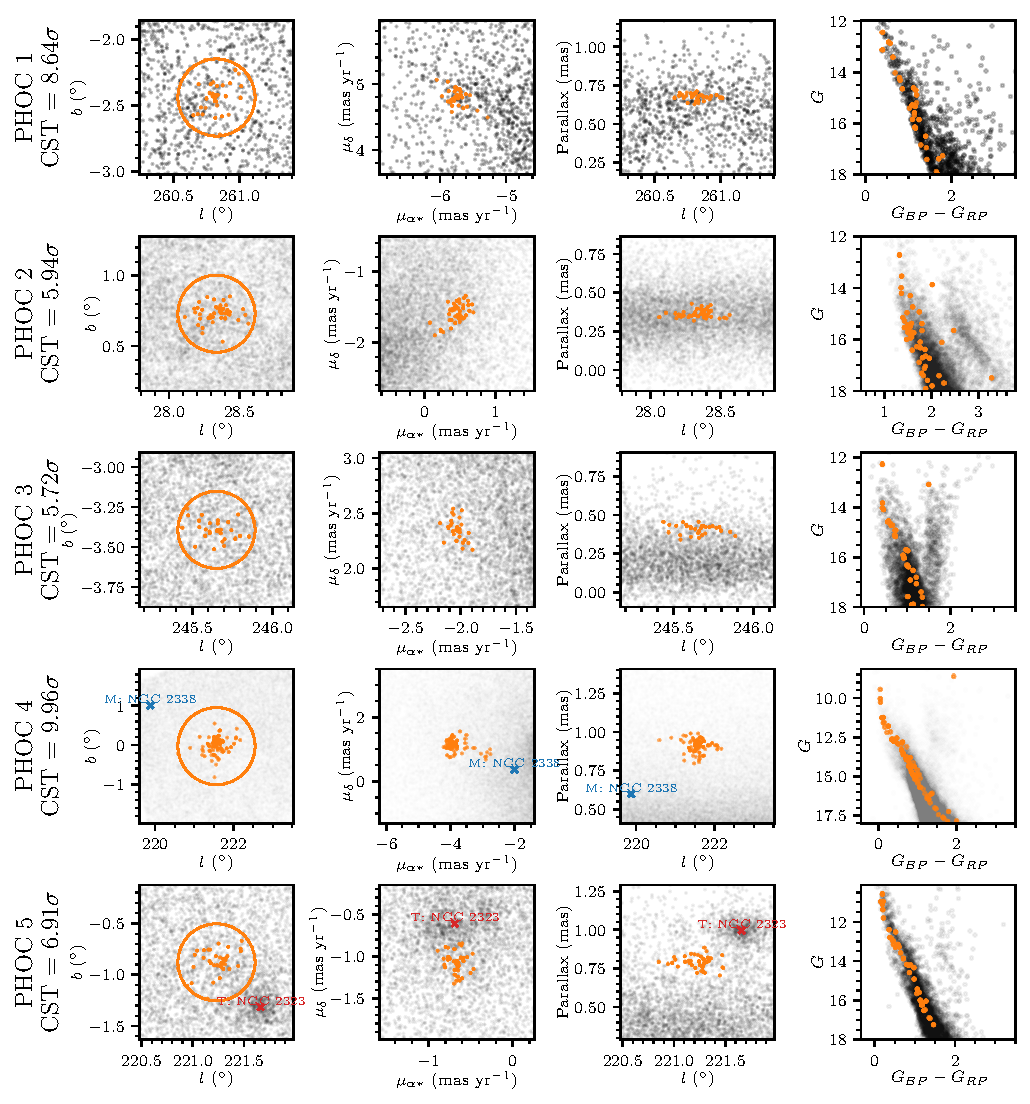
\includegraphics[width=\textwidth]{fig/c2/fig_new_ocs_0.pdf}
   \caption{\reviewtwo{Astrometric and photometric plots of the first five new OCs from Sect.~\ref{c2:sec:new_ocs}. Identified member stars are shown in orange, with background stars in black. Only members with a membership probability of greater than 50\% are plotted. The estimated tidal radius for the OCs is depicted with a circle in the $l$ vs. $b$ plots in the first column. CST scores for each object are shown with its name on the left. Nearby OCs from literature catalogues are marked when visible. T (in red text) denotes sources from \cite{cantat-gaudin_clusters_2020}, while M (blue) and S (purple) denote sources from MWSC and \cite{sim_207_2019} respectively that were not detected by \cite{cantat-gaudin_clusters_2020}. A (brown) denotes new OCs detected recently by \cite{castro-ginard_hunting_2020}.   }}\label{app:c2:fig:new_ocs_0}%
\end{figure*}


\begin{figure*}[ht]
   \centering
   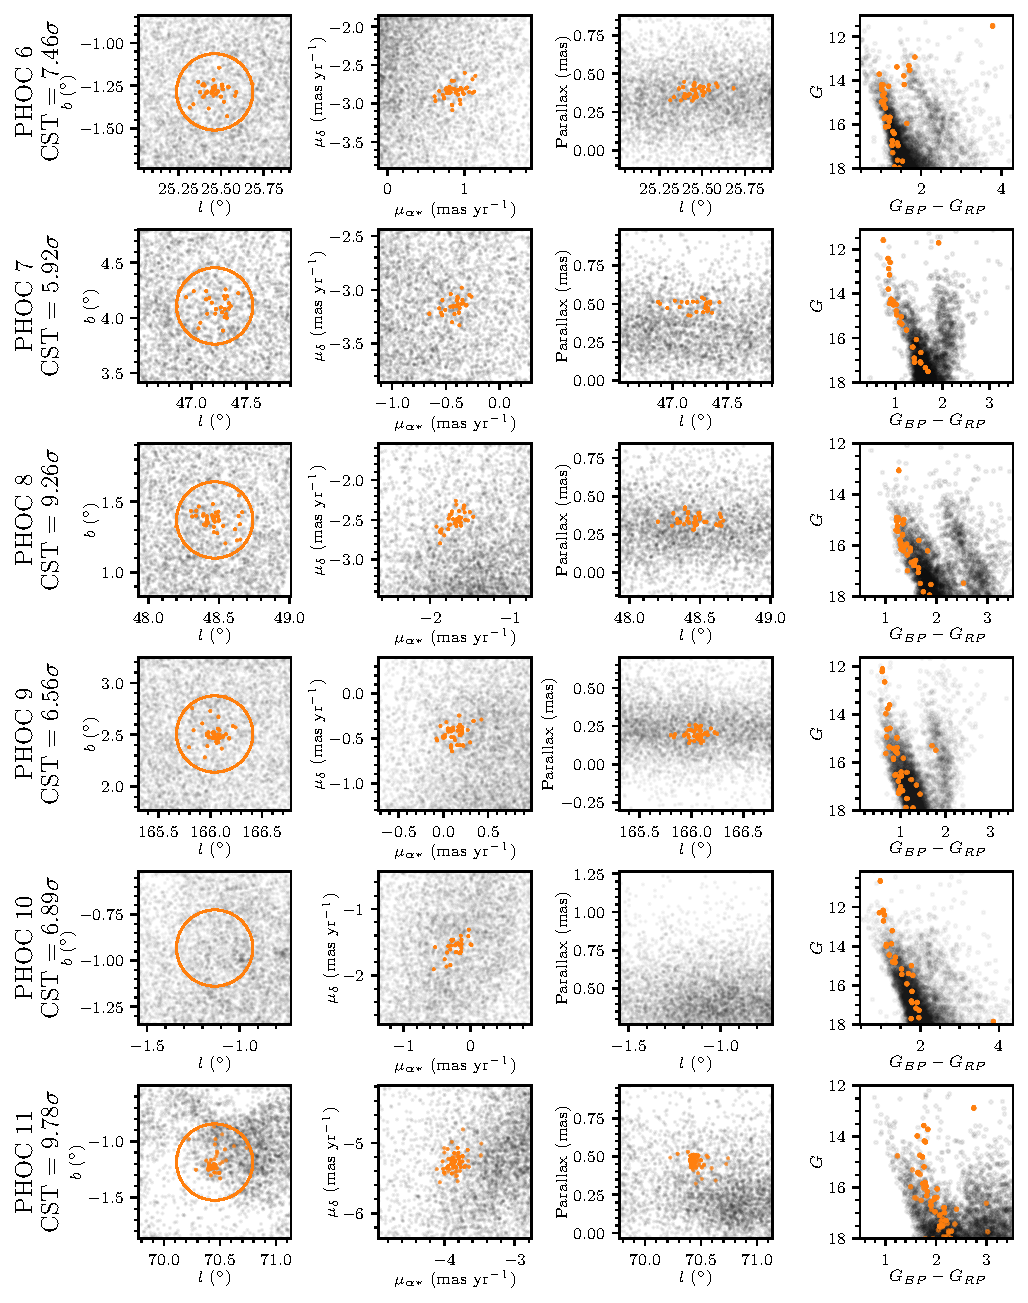
\includegraphics[width=\textwidth]{fig/c2/fig_new_ocs_1.pdf}
   \caption{\reviewtwo{Plots of the new OCs PHOC 6 to 11, plotted in the same style as Fig.~\ref{app:c2:fig:new_ocs_0}. }}%
   \label{app:c2:fig:new_ocs_1}
\end{figure*}

\begin{figure*}[ht]
   \centering
   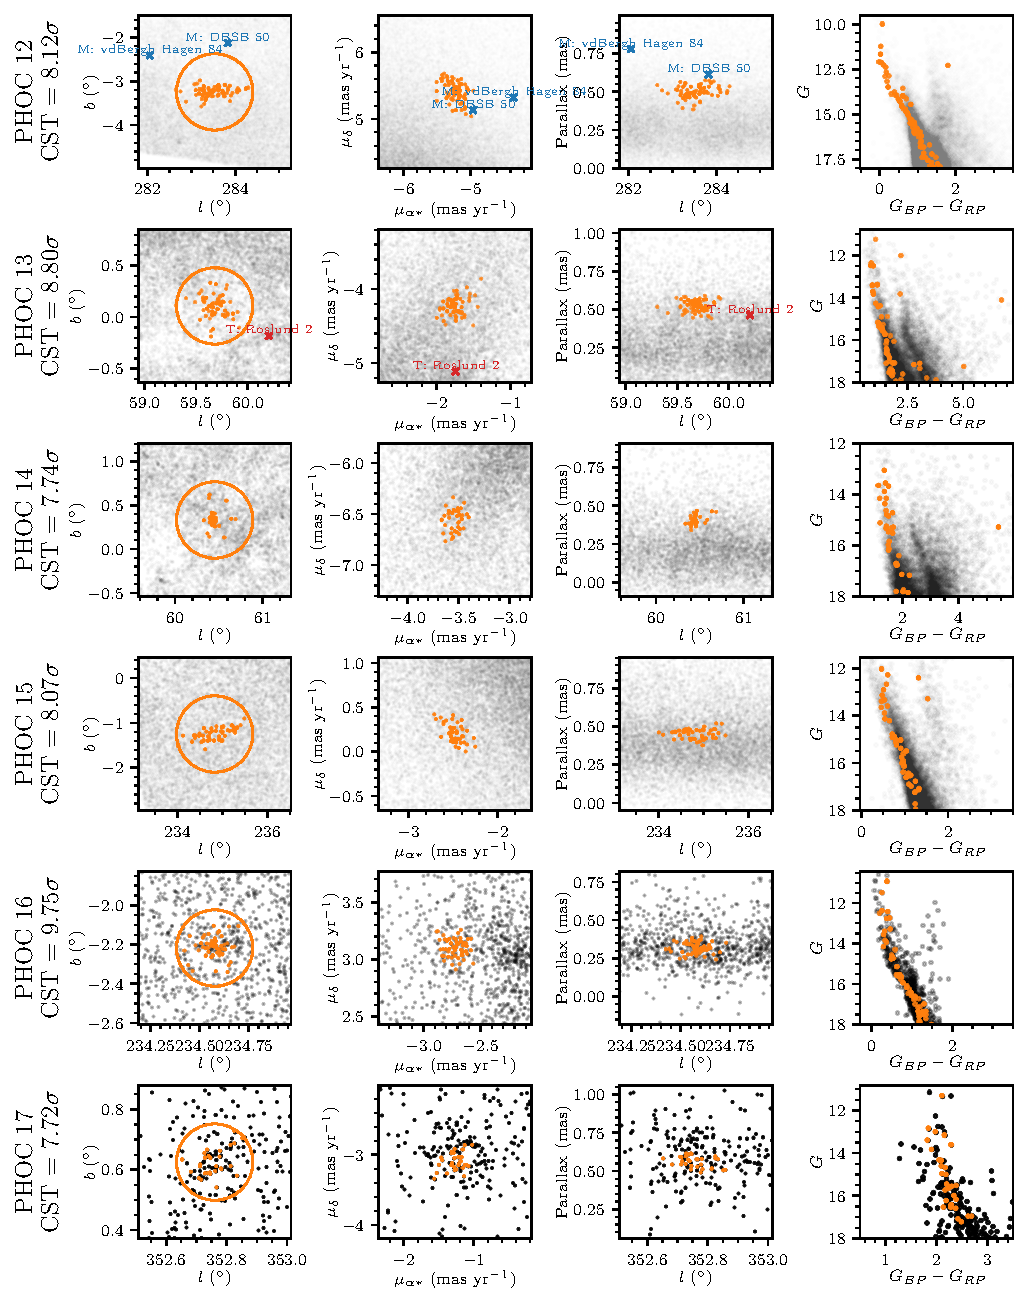
\includegraphics[width=\textwidth]{fig/c2/fig_new_ocs_2.pdf}
   \caption{\reviewtwo{Plots of the new OCs PHOC 12 to 17, plotted in the same style as Fig.~\ref{app:c2:fig:new_ocs_0}. }}%
   \label{app:c2:fig:new_ocs_2}
\end{figure*}

\begin{figure*}[ht]
   \centering
   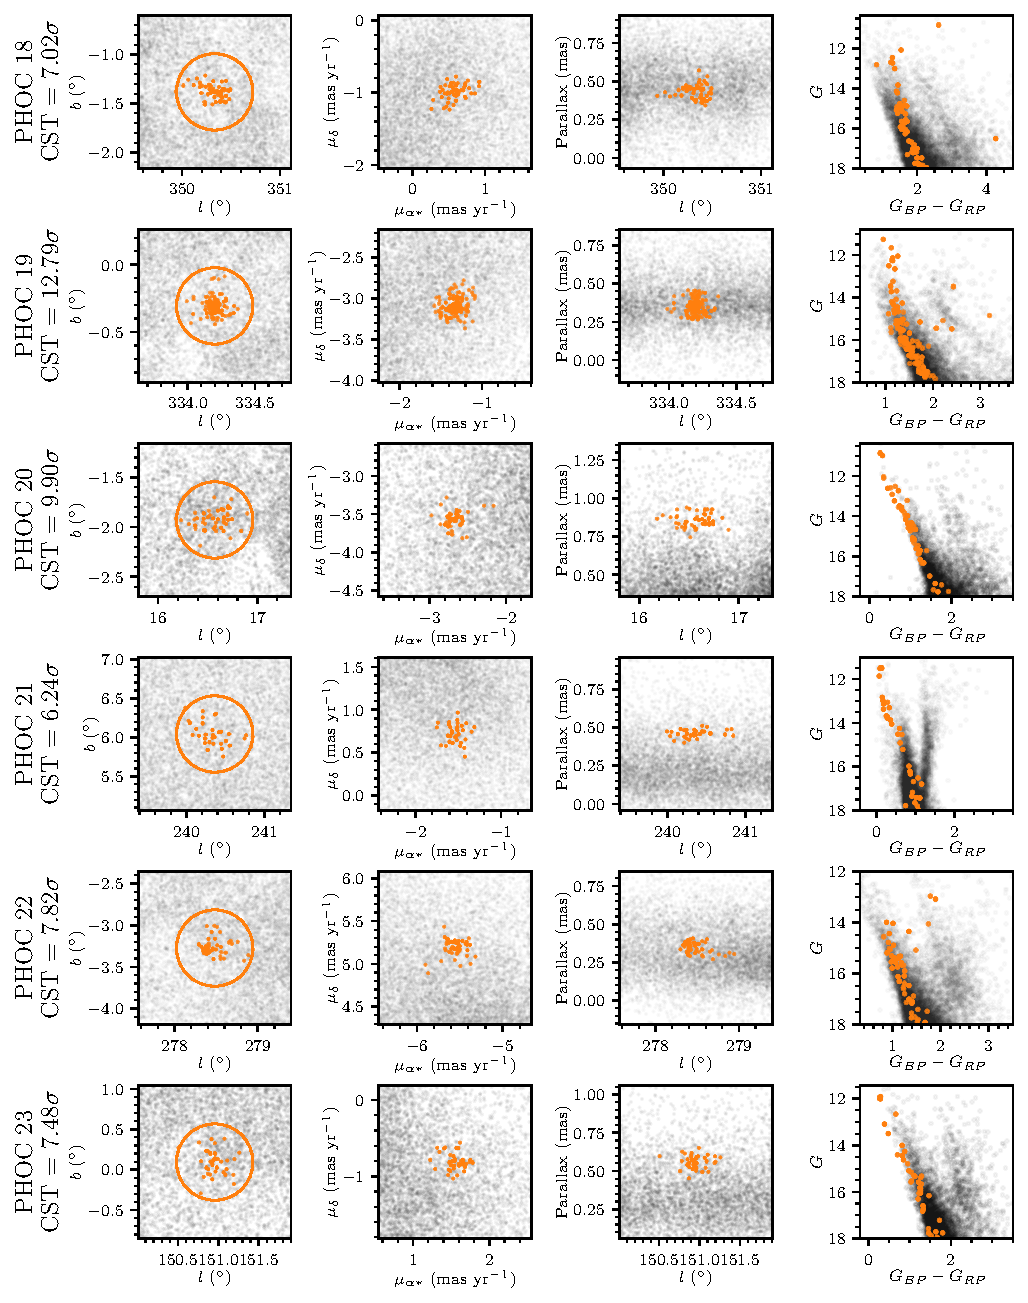
\includegraphics[width=\textwidth]{fig/c2/fig_new_ocs_3.pdf}
   \caption{\reviewtwo{Plots of the new OCs PHOC 18 to 23, plotted in the same style as Fig.~\ref{app:c2:fig:new_ocs_0}. }}%
   \label{app:c2:fig:new_ocs_3}
\end{figure*}

\begin{figure*}[ht]
   \centering
   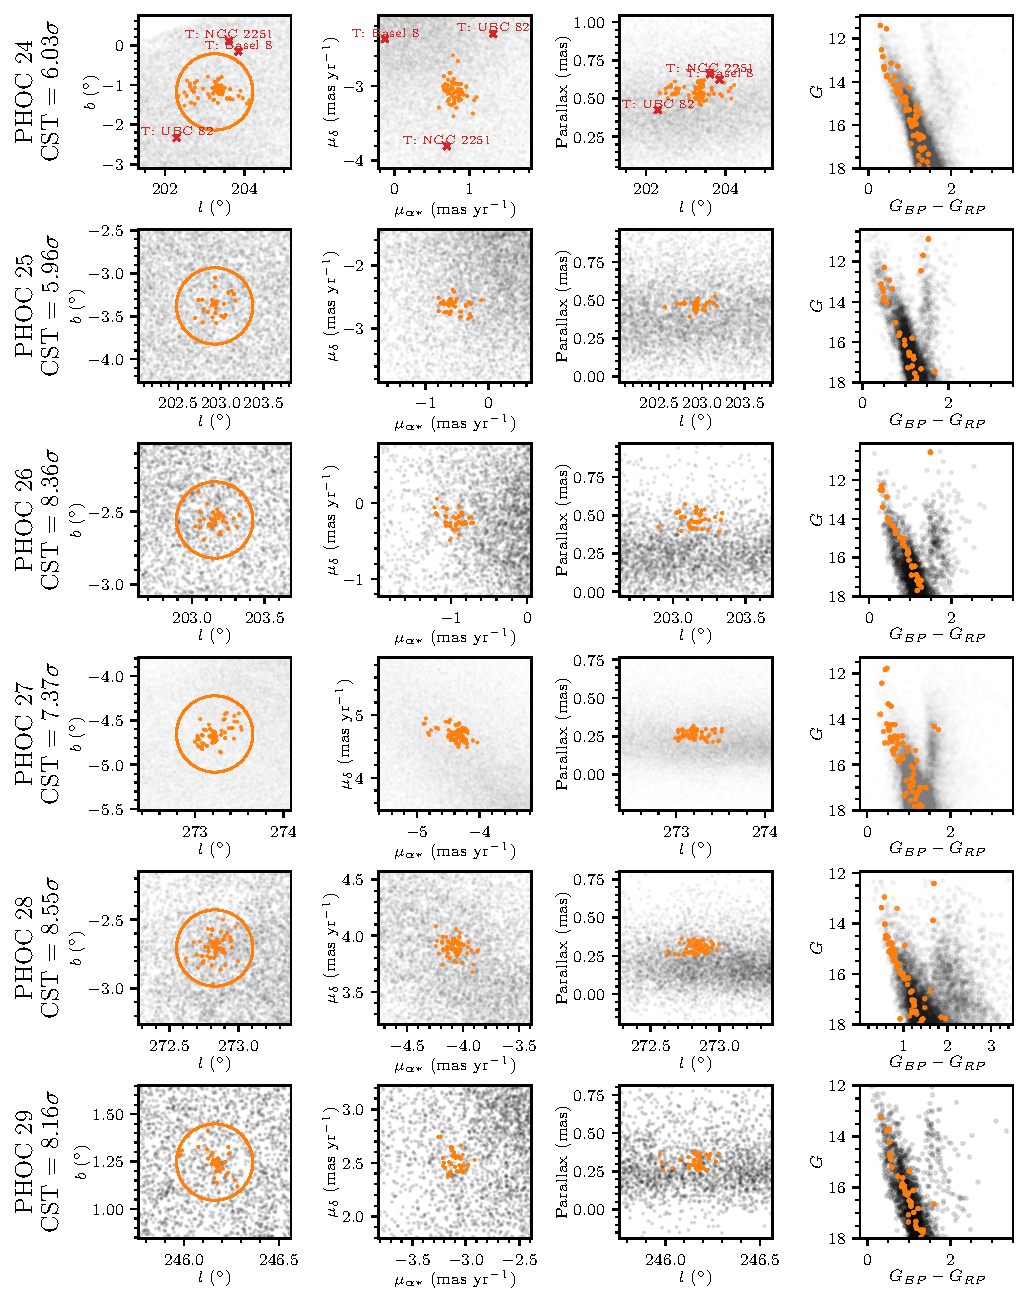
\includegraphics[width=\textwidth]{fig/c2/fig_new_ocs_4.pdf}
   \caption{\reviewtwo{Plots of the new OCs PHOC 24 to 29, plotted in the same style as Fig.~\ref{app:c2:fig:new_ocs_0}. }}%
   \label{app:c2:fig:new_ocs_4}
\end{figure*}

\begin{figure*}[ht]
   \centering
   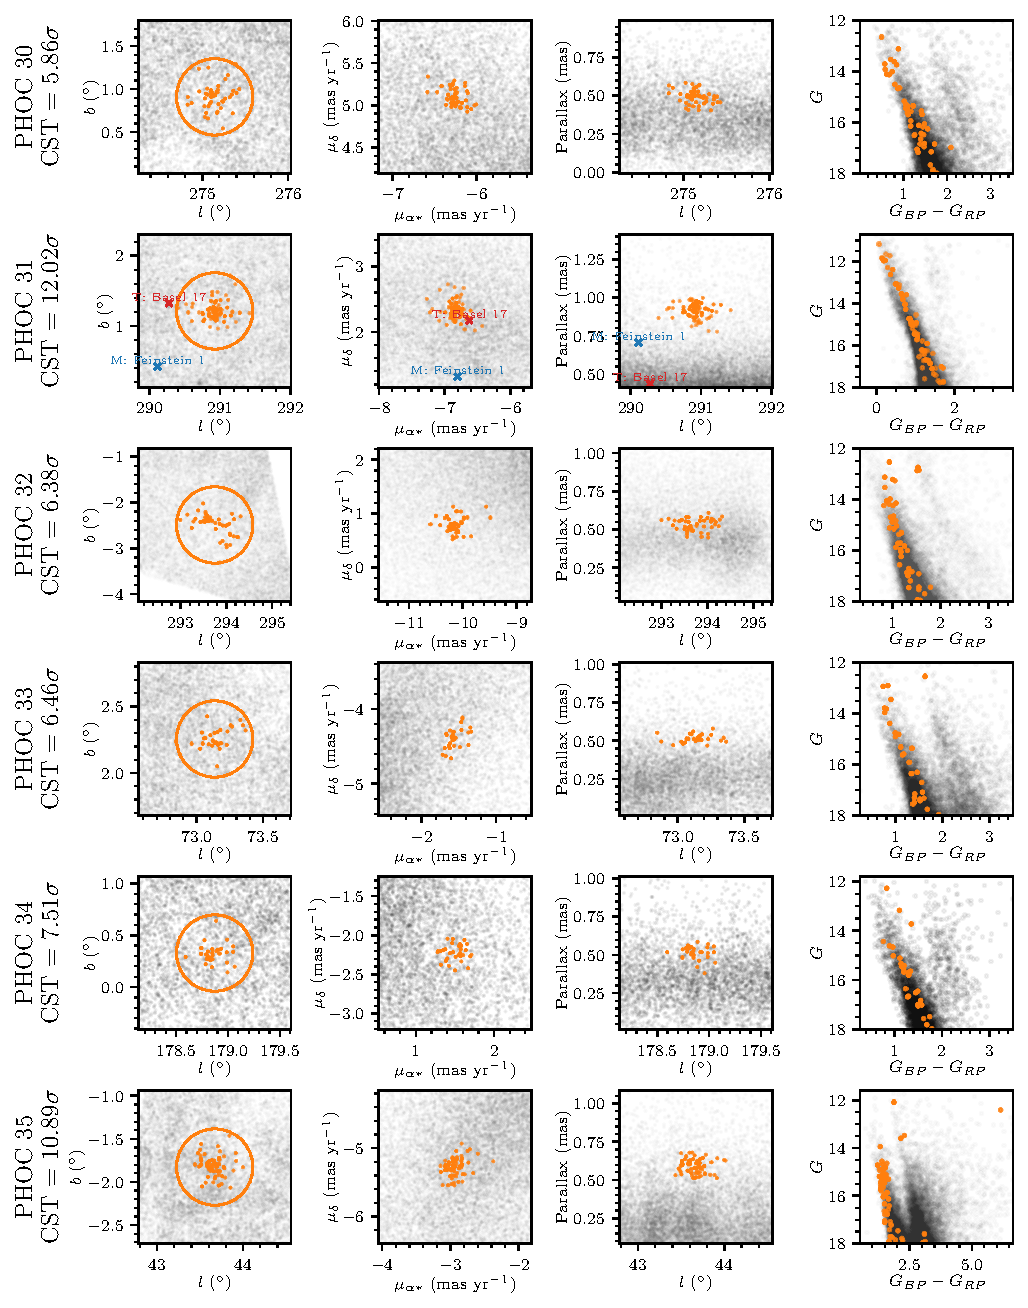
\includegraphics[width=\textwidth]{fig/c2/fig_new_ocs_5.pdf}
   \caption{\reviewtwo{Plots of the new OCs PHOC 30 to 35, plotted in the same style as Fig.~\ref{app:c2:fig:new_ocs_0}. }}%
   \label{app:c2:fig:new_ocs_5}
\end{figure*}

\begin{figure*}[ht]
   \centering
   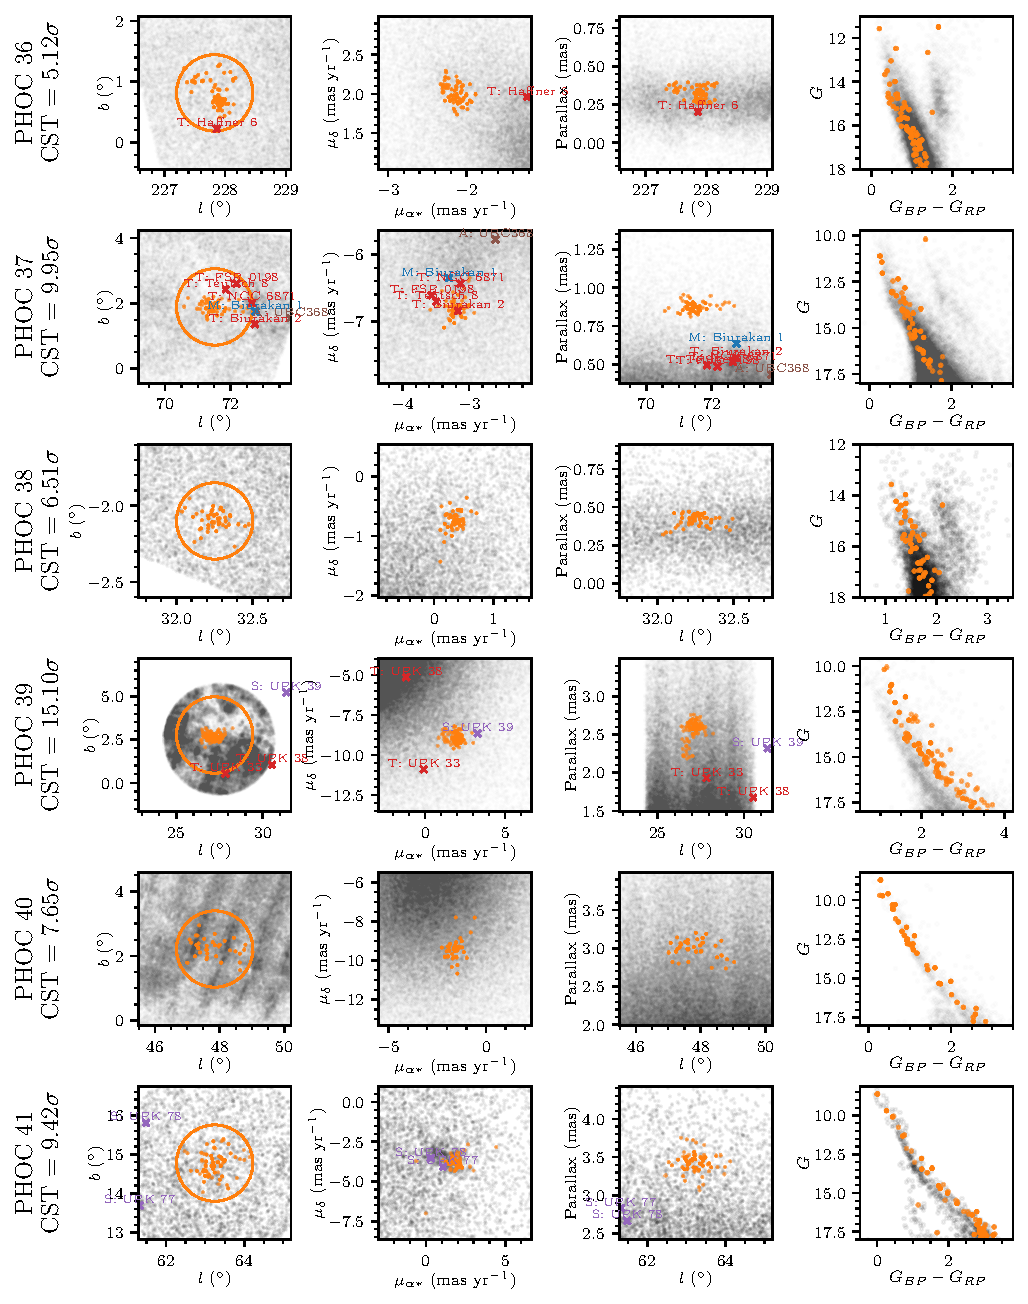
\includegraphics[width=\textwidth]{fig/c2/fig_new_ocs_6.pdf}
   \caption{\reviewtwo{Plots of the new OCs PHOC 36 to 41, plotted in the same style as Fig.~\ref{app:c2:fig:new_ocs_0}. }}%
   \label{app:c2:fig:new_ocs_6}
\end{figure*}




%-------------------------------------------------------------------


\subsection{List of fields used in this study}\label{app:c2:fields}

See Table \ref{app:c2:table:sky_locations}.

\begin{table*}

% Define first header
\caption{\label{app:c2:table:sky_locations}Sky locations and HEALPix indices of the central pixels included in this study.}

\centering
\footnotesize
\begin{tabular}{cccc|cccc}
\hline\hline
Number & $\alpha$ ($^\circ$) & $\delta$ ($^\circ$) & Pixel\tablefootmark{a} & Number & $\alpha$ ($^\circ$) & $\delta$ ($^\circ$) & Pixel\tablefootmark{a} \\
\hline

0  & 313.6 & -12.0 & 12238 & 50 & 318.1 & 46.6  & 3844  \\
1  & 104.1 & 18.2  & 5976  & 51 & 91.4  & 30.0  & 6106  \\
2  & 128.0 & -41.8 & 9817  & 52 & 136.9 & -54.3 & 9434  \\
3  & 343.9 & 69.4  & 3953  & 53 & 357.6 & 61.9  & 3575  \\
4  & 90.0  & 6.0   & 5900  & 54 & 48.1  & 46.6  & 772   \\
5  & 281.2 & -3.6  & 7564  & 55 & 76.5  & 45.0  & 365   \\
6  & 99.8  & 9.6   & 5909  & 56 & 120.9 & -31.4 & 9940  \\
7  & 92.8  & -6.0  & 5364  & 57 & 278.4 & -23.3 & 7243  \\
8  & 98.4  & 6.0   & 5563  & 58 & 293.9 & 22.0  & 3585  \\
9  & 281.2 & -25.9 & 7235  & 59 & 143.7 & -51.3 & 9437  \\
10 & 113.9 & -30.0 & 9946  & 60 & 34.4  & 64.9  & 915   \\
11 & 61.9  & 40.2  & 403   & 61 & 246.1 & -27.3 & 10738 \\
12 & 225.0 & -64.9 & 10432 & 62 & 274.2 & -17.0 & 7278  \\
13 & 106.9 & -8.4  & 5420  & 63 & 169.3 & -58.9 & 9484  \\
14 & 281.2 & -8.4  & 7552  & 64 & 84.4  & 31.4  & 6124  \\
15 & 73.1  & 31.4  & 284   & 65 & 168.2 & -61.9 & 9480  \\
16 & 286.9 & 13.2  & 7663  & 66 & 325.8 & 52.8  & 3860  \\
17 & 80.2  & 41.8  & 346   & 67 & 246.1 & -32.8 & 10702 \\
18 & 78.8  & 48.1  & 378   & 68 & 321.1 & 57.4  & 3870  \\
19 & 268.6 & -30.0 & 7205  & 69 & 302.3 & 35.7  & 3657  \\
20 & 303.8 & 34.2  & 3651  & 70 & 116.7 & -17.0 & 10158 \\
21 & 152.1 & -58.9 & 9340  & 71 & 88.6  & 27.3  & 6094  \\
22 & 120.9 & -10.8 & 5396  & 72 & 272.8 & -31.4 & 7192  \\
23 & 316.6 & 48.1  & 3846  & 73 & 85.8  & 30.0  & 6118  \\
24 & 295.3 & 23.3  & 3588  & 74 & 203.6 & -58.9 & 10427 \\
25 & 319.2 & 35.7  & 3317  & 75 & 48.6  & 52.8  & 792   \\
26 & 357.0 & 67.9  & 3927  & 76 & 315.0 & 46.6  & 3843  \\
27 & 112.5 & -20.7 & 9983  & 77 & 274.2 & 30.0  & 8153  \\
28 & 143.4 & -31.4 & 10004 & 78 & 112.5 & -18.2 & 5376  \\
29 & 272.8 & -18.2 & 7275  & 79 & 299.5 & 30.0  & 3606  \\
30 & 299.5 & 35.7  & 3658  & 80 & 289.7 & 10.8  & 7655  \\
31 & 136.6 & -48.1 & 9462  & 81 & 307.8 & 52.8  & 3875  \\
32 & 157.5 & -57.4 & 9506  & 82 & 98.4  & 23.3  & 6008  \\
33 & 257.3 & -38.7 & 10610 & 83 & 111.1 & -14.5 & 5385  \\
34 & 36.6  & 66.4  & 918   & 84 & 285.5 & 32.8  & 3630  \\
35 & 261.6 & -37.2 & 10612 & 85 & 255.9 & -37.2 & 10616 \\
36 & 204.8 & -60.4 & 10425 & 86 & 272.8 & -8.4  & 7387  \\
37 & 245.0 & -49.7 & 10543 & 87 & 300.9 & 34.2  & 3656  \\
38 & 258.8 & -37.2 & 10611 & 88 & 272.8 & -20.7 & 7272  \\
39 & 310.8 & 12.0  & 3117  & 89 & 23.8  & 64.9  & 911   \\
40 & 277.0 & -14.5 & 7290  & 90 & 102.7 & 0.0   & 5530  \\
41 & 122.3 & -22.0 & 10126 & 91 & 317.8 & 40.2  & 3496  \\
42 & 278.4 & 23.3  & 8056  & 92 & 109.7 & -31.4 & 9956  \\
43 & 105.5 & -19.5 & 5209  & 93 & 165.0 & -58.9 & 9483  \\
44 & 146.7 & -55.9 & 9428  & 94 & 95.6  & -10.8 & 5331  \\
45 & 91.4  & 19.5  & 5994  & 95 & 71.7  & 41.8  & 361   \\
46 & 61.7  & 49.7  & 439   & 96 & 253.1 & -34.2 & 10704 \\
47 & 319.2 & 38.7  & 3490  & 97 & 282.7 & 0.0   & 7578  \\
48 & 193.1 & -43.4 & 10904 & 98 & 95.6  & -23.3 & 5216  \\
49 & 97.0  & 7.2   & 5905  & 99 & 119.5 & -24.6 & 10122 \\


\hline

\end{tabular}

\normalsize

\tablefoot{
\tablefoottext{a}{Index of the level 5 HEALPix pixel of the field. To reproduce each full field, the eight nearest neighbour HEALPix level 5 pixels must also be selected.}
}

\end{table*}


\clearpage


\section{Appendices for Chapter \ref{sec:census}}

\subsection{Description of contents of online tables}\label{app:c3:tables}

We provide tables of clusters, rejected clusters, member stars, and members stars for rejected clusters at the CDS. Tables of clusters follow the table format in Table~\ref{app:c3:tab:cluster_lists}. Tables of members follow the same columns and column naming scheme as in \emph{Gaia} DR3 \citep{gaia_collaboration_gaia_2022}, except while also having columns referencing the cluster name and cluster ID we assign them to, the cluster membership probability, and a flag for if the star is a member within our estimated tidal radius $r_t$.

% Cluster lists table
\begin{table}
\caption{Description of the columns in the tables of detected clusters.\label{app:c3:tab:cluster_lists}}
\centering
\begin{tabular}{c c c l}
\hline\hline
Col. & Label & Unit & Description \\
\hline          
% Name and designation
1     & Name                  & --  & Designation \\
2     & Internal ID           & --  & Internal designation \\
3     & All names             & --  & All literature names \\
4     & Kind                  & --  & Estimated object type\tablefootmark{c} \\
5     & $n_\text{stars}$      & --  & Num. of member stars \\
6     & $\text{S/N}$          & --  & Astrometric S/N \\
7     & $n_\text{stars}|_{r_\text{t}}$ & --  & $n_\text{stars}$ within $r_t$ \\
8     & $\text{S/N}|_{r_\text{t}}$ & --  & $\text{S/N}$ within $r_t$ \\
\hline

% Position, radii
9-10     & $\alpha$, $\delta$ & deg & ICRS position \\
11-12    & $l$, $b$           & deg & Galactic position \\
13-16    & $r_{50,\,c,\,t,\,\text{tot}}$ & deg & Angular radii \\
17-20    & $R_{50,\,c,\,t,\,\text{tot}}$ & pc & Physical radii \\

% Other astrometry and distance stuff
21-26\tablefootmark{a} & $\mu_{\alpha^*}$, $\mu_\delta$ & mas yr$^{-1}$ & ICRS proper motions \\
27-29\tablefootmark{a} & $\varpi$              & mas & Parallax \\
30-32\tablefootmark{b} & $d$                   & pc  & Distance \\
33    & $n_d$                 & pc  & $n_\text{stars}$ for distance calc. \\
34    & $\varpi_0$ type       & --  & Parallax offset type\tablefootmark{d} \\
35-37 & $X$, $Y$, $Z$         & pc  & Galactocentric coords. \\

% RVs
38-40\tablefootmark{a} & RV   & km s$^{-1}$ & Radial velocity\tablefootmark{e} \\
41    & $n_\text{RV}$         & --  & $n_\text{stars}$ with RVs \\
\hline

% CMD classifier
42-46\tablefootmark{b} & CMD class & --  & CMD class quantiles\tablefootmark{f} \\
47    & Human class           & --  & (where available)\tablefootmark{f} \\

% AgeNN
48-50\tablefootmark{b} & $\log t$              & $\log \left[ \text{yr} \right]$  & Cluster age \\
51-53\tablefootmark{b} & $A_V$                 & mag & V-band extinction \\
54-56\tablefootmark{b} & $\Delta A_V$        & mag & Differential $A_V$ \\
57-59\tablefootmark{b} & $m-M$                 & mag & Photometric dist. mod. \\
\hline

% Other stuff
60    & $m_{clSize}$          & --  & HDBSCAN parameter \\
61    & \texttt{merged}  & --  & Flag if merged\tablefootmark{g} \\
62    & \texttt{is\_gmm}  & --  & Flag if GMM used\tablefootmark{h} \\
63    & $n_\text{crossmatches}$ & --  & Num. crossmatches \\
64    & Xmatch type  & --  & Type of crossmatch\tablefootmark{i} \\

\hline
\end{tabular}

\tablefoot{The full version is available at the CDS.
\tablefoottext{a}{Mean value, standard deviation $\sigma$, and standard error $\sigma \, / \sqrt{n}$ are given.}
\tablefoottext{b}{Median value and various confidence intervals are given.}
\tablefoottext{c}{\texttt{g} for objects in the \cite{vasiliev_gaia_2021} GC catalogue, otherwise \texttt{o} (OC) or \texttt{m} (moving group) for clusters according to the empirical cuts in \cite{cantat-gaudin_clusters_2020}.}
\tablefoottext{d}{Flag indicating six clusters for which parallax bias correction using the method of \cite{lindegren_gaia_2021} was not possible, and a global offset was used instead (see Sect.~\ref{c3:sec:clustering:parameters}).}
\tablefoottext{e}{Corrected using cluster distances to be relative to cluster centre.}
\tablefoottext{f}{Cluster CMD classes derived using the neural network in Sect.~\ref{c3:sec:cmd_classifier}.}
\tablefoottext{g}{Indicates 25 clusters merged by hand (see Sect.~\ref{c3:sec:clustering}).}
\tablefoottext{h}{Indicates nine clusters with members from an additional Gaussian mixture model clustering step.}
\tablefoottext{i}{Method used to assign name to cluster (see Sect.~\ref{c3:sec:crossmatching:names}.)}
}

\end{table}

\subsection{Table of crossmatch results}\label{app:c3:crossmatches}

% Cluster lists table
\begin{sidewaystable}[p]
\caption{All cluster crossmatches, including literature clusters that have no match.\label{app:c3:tab:all_crossmatches}}
\centering
\begin{tabular}{*{12}{c}}
\hline\hline
ID & Name & Source & Type & $\theta$ & $\theta_r$\tablefootmark{a} & $s_{\mu_{\alpha*}}$ & $\sigma_{\mu_{\alpha*}}$ & $s_{\mu_{\delta}}$ & $\sigma_{\mu_{\delta*}}$ & $s_{\varpi}$ & $\sigma_{\varpi}$ \\
& & & & ($^\circ$) & & (mas yr$^{-1}$) & & (mas yr$^{-1}$) & & (mas) \\
	
\hline

\multicolumn{12}{c}{$\cdot \cdot \cdot$} \\ 

% 176 & Basel 1 & Cantat-Gaudin+20 & gaia dr2 & 0.01 & 0.04 & 0.03 & 0.00 & 0.01 & 0.00 & 0.01 & 0.00\\
% 176 & Basel 1 & Dias+02 & position & 0.03 & 0.12 & - & - & - & - & - & -\\
% 176 & Basel 1 & Kharchenko+13 & hipparcos & 0.01 & 0.04 & 0.40 & 0.09 & 1.04 & 0.24 & 0.06 & 0.17\\
179 & Basel 10 & Bica+18 & position & 0.01 & 0.04 & - & - & - & - & - & -\\
179 & Basel 10 & Dias+02 & position & 0.01 & 0.04 & - & - & - & - & - & -\\
179 & Basel 10 & Cantat-Gaudin+20 & gaia dr2 & 0.01 & 0.07 & 0.03 & 0.00 & 0.05 & 0.01 & 0.01 & 0.00\\
179 & Basel 10 & Kharchenko+13 & hipparcos & 0.01 & 0.07 & 0.30 & 0.05 & 2.49 & 0.51 & 0.02 & 0.00\\
179 & Basel 10 & Kharchenko+13 & position & 0.01 & 0.07 & - & - & - & - & - & -\\
183 & Basel 11A & Cantat-Gaudin+20 & gaia dr2 & 0.01 & 0.01 & 0.02 & 0.00 & 0.05 & 0.00 & 0.02 & 0.00\\
183 & Basel 11A & Kharchenko+13 & hipparcos & 0.01 & 0.04 & 0.52 & 0.12 & 1.66 & 0.42 & 0.11 & 0.81\\
183 & Basel 11A & Dias+02 & position & 0.02 & 0.06 & - & - & - & - & - & -\\
183 & Basel 11A & Bica+18 & position & 0.03 & 0.06 & - & - & - & - & - & -\\
183 & Basel 11A & Kharchenko+13 & position & 0.01 & 0.04 & - & - & - & - & - & -\\
3003 & Basel 11B & Kharchenko+13 & position & 0.11 & 0.25 & - & - & - & - & - & -\\
184 & Basel 11B & Kharchenko+13 & hipparcos & 0.02 & 0.06 & 1.28 & 0.37 & 0.24 & 0.06 & 0.17 & 1.40\\
184 & Basel 11B & Kharchenko+13 & position & 0.02 & 0.06 & - & - & - & - & - & -\\
184 & Basel 11B & Dias+02 & position & 0.01 & 0.02 & - & - & - & - & - & -\\
184 & Basel 11B & Cantat-Gaudin+20 & gaia dr2 & 0.01 & 0.03 & 0.02 & 0.00 & 0.01 & 0.00 & 0.03 & 0.00\\
184 & Basel 11B & Bica+18 & position & 0.00 & 0.01 & - & - & - & - & - & -\\
6363 & Basel 11B & Kharchenko+13 & hipparcos & 0.11 & 0.39 & 2.15 & 0.64 & 1.99 & 0.59 & 0.22 & 1.98\\
6363 & Basel 11B & Kharchenko+13 & position & 0.11 & 0.39 & - & - & - & - & - & -\\
% - & Basel 12 & Dias+02 & position & - & - & - & - & - & - & - & -\\
% - & Basel 12 & Kharchenko+13 & hipparcos & - & - & - & - & - & - & - & -\\
% - & Basel 12 & Bica+18 & position & - & - & - & - & - & - & - & -\\
% 180 & Basel 13 & Kharchenko+13 & position & 0.11 & 0.74 & - & - & - & - & - & -\\
% - & Basel 13A & Bica+18 & position & - & - & - & - & - & - & - & -\\
% - & Basel 14 & Dias+02 & position & - & - & - & - & - & - & - & -\\
% - & Basel 14 & Kharchenko+13 & hipparcos & - & - & - & - & - & - & - & -\\
% - & Basel 15 & Bica+18 & position & - & - & - & - & - & - & - & -\\
% - & Basel 15 & Kharchenko+13 & hipparcos & - & - & - & - & - & - & - & -\\
% - & Basel 15 & Dias+02 & position & - & - & - & - & - & - & - & -\\
% 181 & Basel 17 & Kharchenko+13 & position & 0.00 & 0.02 & - & - & - & - & - & -\\
% 181 & Basel 17 & Cantat-Gaudin+20 & gaia dr2 & 0.01 & 0.07 & 0.01 & 0.00 & 0.06 & 0.08 & 0.01 & 0.00\\
% 181 & Basel 17 & Kharchenko+13 & hipparcos & 0.00 & 0.02 & 0.62 & 0.10 & 2.37 & 0.43 & 0.11 & 0.93\\
% 181 & Basel 17 & Dias+02 & position & 0.00 & 0.02 & - & - & - & - & - & -\\

\multicolumn{12}{c}{$\cdot \cdot \cdot$} \\ 

\hline
\end{tabular}

\tablefoot{The full version is available at the CDS; the above only shows crossmatches against a selection of Basel clusters. Depending on the type of work crossmatched against, only separations in terms of position $\theta$ may be listed. For works with astrometry, separations $s$ with respect to $\mu_{\alpha*}$, $\mu_\delta$, and $\varpi$ are shown, in addition to separations $\sigma$ which are in terms of standard deviations about the mean of the astrometry of these clusters added together in quadrature, after accounting for worst-case systematics. Cluster entries in the literature that did not have a valid crossmatch against any cluster detected in this study are listed with only the name, source, and source type columns filled. Recalling Sect.~\ref{c3:sec:crossmatching}, for a valid crossmatch, we require $\theta_r < 1$, and additionally, when crossmatching to a work with full five parameter astrometry, all $\sigma$ values to be less than two. 
\tablefoottext{a}{The separation between cluster centres in terms of the largest cluster radius available, $\theta_r = \theta / \text{max}(r_t, \, r_{t,\,\text{lit}})$}
}

\end{sidewaystable}

Here we provide a table of all crossmatches to all literature clusters that meet our adopted crossmatch criteria from Sect.~\ref{c3:sec:crossmatching} in Table~\ref{app:c3:tab:all_crossmatches}. For every cluster in the literature that we detect in this work, the table lists the internal cluster ID corresponding to our table of clusters in Table~\ref{c3:tab:catalogue} that corresponds to this object. For clusters that we do not redetect, only a blank row with the cluster name, source paper, and type of crossmatch is shown.


\subsection{Bayesian neural networks}\label{app:c3:bayesian_nets}

Given that Bayesian neural networks (BNNs) are only just beginning to see use in the astronomical literature \citep[e.g.][]{huertas-company_hubble_2019}, here we provide a brief background overview of the advantages and caveats of the approximate BNN methodology we adopted in Sect.~\ref{c3:sec:cmd_classifier} and Sect.~\ref{c3:sec:agenn}.

BNNs are a somewhat elusive area of open research in machine learning. Their appeal is clear: unlike a deterministic approach or an approach based on simply perturbing network inputs, a perfect BNN would be able to estimate both aleatoric uncertainties, which are uncertainties that result from random phenomena, such as uncertainty on photometric measurements; and epistemic uncertainties, which are uncertainties that result from a lack of knowledge about the underlying processes being modelled. For instance, any remaining gaps or issues in the simulated training data we use would cause a traditional deterministic neural network to always output an incorrect answer, whereas a probabilistic neural network should at least output a wide range of answers that demonstrate its uncertainty in such difficult cases (\cite{goan_bayesian_2020}, \cite{jospin_hands-bayesian_2022}).

In practice, there is currently no perfect BNN architecture, with all approaches having some flaws (\cite{goan_bayesian_2020}, \cite{jospin_hands-bayesian_2022}). While a Monte-Carlo Markov chain (MCMC)-based approach should in theory be superior, where every network weight has an arbitrary posterior distribution, MCMC-based BNNs are extremely difficult or impossible to train accurately, with current sampling techniques being inadequate \citep{goan_bayesian_2020}. In addition, BNNs are often time consuming to train. Instead, `variational inference' is widely used to approximate BNNs. In this technique, an ideal BNN is approximated by perturbing network features, approximating a BNN by `emphasising or de-emphasising' certain parts of a trained model when the model is sampled. This can then be used to estimate the epistemic uncertainty of a model by sampling a variational network multiple times.

Many approaches for variational inference exist in the literature, with a common approach being dropout regularisation as an approximation of a BNN \citep{gal_dropout_2015-1}, having also been used within astronomy (e.g. \cite{huertas-company_hubble_2019}, \cite{leung_deep_2019}). However, this approximation is not inherently Bayesian \citep{hron_variational_2017}, and may be improved upon with recent developments in the literature. Another common approximation is to assume that all layer kernel and bias weights are drawn from simple distributions, such as independent Gaussian distributions. This allows for gradients during network training to be calculated straightforwardly using Bayes by backpropagation \citep{blundell_weight_2015}. This approximation can hold relatively well for (simple) neural networks, which often have normally distributed weights, but may cause underfitting on more complicated problems \citep{goan_bayesian_2020}. Due to the time-consuming nature of repeated samples of all kernel and bias posterior distributions, we also apply an approximation known as Flipout to more efficiently sample them with a lower runtime while preserving good training characteristics \citep{wen_flipout_2018}. Similar approaches using Bayes by backpropagation and Flipout have seen some use in the astronomy literature \citep[e.g.][]{lin_detection_2021}. We use the implementations of \texttt{DenseFlipout} and \texttt{Convolution2DFlipout} layers in TensorFlow Probability \citep{dillon_tensorflow_2017}, minimising the evidence lower bound (ELBO) loss \citep{blundell_weight_2015}.

In initial tests, these approximations produced network outputs with reliable uncertainty estimates that correspond well to the uncertainty inherent to classifying star cluster CMDs. It is worth noting from the literature that variational-inference based approaches are still more overconfident than a true BNN when applied to unseen data \citep{goan_bayesian_2020}, and that this approach is still an imperfect estimator of the true uncertainty of our model; nevertheless, our adopted method was found to be as accurate as a traditional deterministic network architecture of the same configuration when applied to our training data, but while providing an estimate of its uncertainty and without dramatically increasing runtime during training or sampling.
       % INCLUDE: appendix

\cleardoublepage
% !TEX root = ../my-thesis.tex
%
\pagestyle{empty}
\hfill
\vfill
\pdfbookmark[0]{Colophon}{Colophon}
\section*{Colophon}

This thesis was typeset with \LaTeXe.
It uses the \textit{Clean Thesis} style developed by Ricardo Langner.
The design of the \textit{Clean Thesis} style is inspired by user guide documents from Apple Inc.

Download the \textit{Clean Thesis} style at \url{http://cleanthesis.der-ric.de/}.


% \cleardoublepage
% % !TEX root = ../my-thesis.tex
%
%************************************************
% Declaration
%************************************************
\pdfbookmark[0]{Declaration}{Declaration}
\addchap{Declaration}
\label{sec:declaration}
\thispagestyle{empty}

You can put your declaration here, to declare that you have completed your work solely and only with the help of the references you mentioned.

\bigskip

\noindent\textit{\thesisUniversityCity, \thesisDate}

\smallskip

\begin{flushright}
	\begin{minipage}{5cm}
		\rule{\textwidth}{1pt}
		\centering\thesisName
	\end{minipage}
\end{flushright}

%*****************************************
%*****************************************

% \clearpage

\newpage

% textwidth in in: \printinunitsof{in}\prntlen{\textwidth}

% textheight in in: \printinunitsof{in}\prntlen{\textheight}

\mbox{}

% **************************************************
% End of Document CONTENT
% **************************************************
\end{document}
